\documentclass[a4paper]{article}
\usepackage{a4wide,amssymb,epsfig,latexsym,multicol,array,hhline,fancyhdr}
\usepackage[utf8]{vntex}
\usepackage{amsmath}
\usepackage{lastpage}
\usepackage[lined,boxed,commentsnumbered]{algorithm2e}
\usepackage{enumerate}
\usepackage{color}
\usepackage{graphicx}							% Standard graphics package
\usepackage{array}
\usepackage{tabularx, caption}
\usepackage{multirow}
\usepackage{multicol}
\usepackage{rotating}
\usepackage{graphics}
\usepackage{geometry}
\usepackage{setspace}
\usepackage{epsfig}
\usepackage{tikz}
\usepackage{ifthen}
\usepackage{float}
\usepackage{listings}
\usepackage{indentfirst}
\usepackage{tabularray}
\usepackage[utf8]{inputenc}
\usetikzlibrary{arrows,snakes,backgrounds}
\usepackage{hyperref}
\hypersetup{urlcolor=blue,linkcolor=black,citecolor=black,colorlinks=true} 
%\usepackage{pstcol} 								% PSTricks with the standard color package

\newtheorem{theorem}{{\bf Theorem}}
\newtheorem{property}{{\bf Property}}
\newtheorem{proposition}{{\bf Proposition}}
\newtheorem{corollary}[proposition]{{\bf Corollary}}
\newtheorem{lemma}[proposition]{{\bf Lemma}}

\definecolor{codegreen}{rgb}{0,0.6,0}
\definecolor{codegray}{rgb}{0.5,0.5,0.5}
\definecolor{codepurple}{rgb}{0.58,0,0.82}
\definecolor{backcolour}{rgb}{0.95,0.95,0.92}
\lstdefinestyle{codingstyle}{
  backgroundcolor=\color{backcolour},
  commentstyle=\color{codegreen},
  keywordstyle=\color{magenta},
  numberstyle=\tiny\color{codegray},
  stringstyle=\color{codepurple},
  basicstyle=\ttfamily\normalsize,
  breakatwhitespace=false,         
  breaklines=true,                 
  captionpos=b,                    
  keepspaces=true,                 
  numbers=left,                    
  numbersep=5pt,                  
  showspaces=false,                
  showstringspaces=false,
  showtabs=false,                  
  tabsize=2,
  language=C
}

\lstset{style=codingstyle}


\AtBeginDocument{\renewcommand*\contentsname{Contents}}
\AtBeginDocument{\renewcommand*\refname{References}}
%\usepackage{fancyhdr}
\setlength{\headheight}{40pt}
\pagestyle{fancy}
\fancyhead{} % clear all header fields
\fancyhead[L]{
 \begin{tabular}{rl}
    \begin{picture}(25,15)(0,0)
    \put(0,-8){
\includegraphics[width=8mm, height=8mm]{hcmut.png}}
    %\put(0,-8){\epsfig{width=10mm,figure=hcmut.eps}}
   \end{picture}&
	%
\includegraphics[width=8mm, height=8mm]{hcmut.png} & %
	\begin{tabular}{l}
		\textbf{\bf \ttfamily Trường Đại học Bách Khoa - ĐHQG Hồ Chí Minh}\\
		\textbf{\bf \ttfamily Khoa Khoa học và Kỹ thuật máy tính}
	\end{tabular} 	
 \end{tabular}
}
\fancyhead[R]{
	\begin{tabular}{l}
		\tiny \bf \\
		\tiny \bf 
	\end{tabular}  }
\fancyfoot{} % clear all footer fields
\fancyfoot[L]{\scriptsize \ttfamily ĐỒ ÁN TỐT NGHIỆP}
\fancyfoot[R]{\scriptsize \ttfamily Trang {\thepage}}


\renewcommand{\headrulewidth}{0.3pt}
\renewcommand{\footrulewidth}{0.3pt}

%%%
\setcounter{secnumdepth}{4}
\setcounter{tocdepth}{3}
\makeatletter
\newcounter {subsubsubsection}[subsubsection]
\renewcommand\thesubsubsubsection{\thesubsubsection .\@alph\c@subsubsubsection}
\newcommand\subsubsubsection{\@startsection{subsubsubsection}{4}{\z@}%
                                     {-3.25ex\@plus -1ex \@minus -.2ex}%
                                     {1.5ex \@plus .2ex}%
                                     {\normalfont\normalsize\bfseries}}
\newcommand*\l@subsubsubsection{\@dottedtocline{3}{10.0em}{4.1em}}
\newcommand*{\subsubsubsectionmark}[1]{}
\makeatother

\begin{document}

\begin{titlepage}
\begin{center}
ĐẠI HỌC QUỐC GIA TP.HỒ CHÍ MINH \\
ĐẠI HỌC BÁCH KHOA \\
KHOA KHOA HỌC VÀ KĨ THUẬT MÁY TÍNH
\end{center}

\vspace{1cm}

\begin{figure}[h!]
\begin{center}

\includegraphics[width=3cm]{hcmut.png}
\end{center}
\end{figure}

\vspace{1cm}

\begin{center}
\textbf{\Large ĐỒ ÁN TỐT NGHIỆP}\\
\hrulefill \\
\vspace{.3cm}
\textbf{\Large Đề tài}\\
\vspace{.3cm}
\textbf{\Large THIẾT BỊ CHUYỂN ĐỔI NGÔN NGỮ KÝ HIỆU SANG GIỌNG NÓI SỬ DỤNG FLEX SENSORS KẾT HỢP VỚI HỌC MÁY
 } \\
\hrulefill
\end{center}


\vspace{3cm}

\begin{table}[h]
\begin{tabular}{rrl}
\hspace{5 cm} & GVHD: & ThS. Trần Thanh Bình\\
& &  ThS. Lê Trọng Nhân  \\
& SVTH: & Lê Nhật Tiến - 1912196 \\
& & Nguyễn Duy Hòa - 2010276  \\
& & \\
\end{tabular}
\end{table}

\begin{center}
{\footnotesize TP. Hồ Chí Minh, tháng 11 năm 2024}
\end{center}
\end{titlepage}


%\thispagestyle{empty}
\pagenumbering{Roman}
\setcounter{page}{1}

\newpage
\section*{Lời cam đoan}
\addcontentsline{toc}{section}{Lời cam đoan}

\indent Chúng tôi xin cam đoan rằng những nội dung trình bày trong báo cáo luận văn này là công trình nghiên cứu của nhóm dưới sự hướng dẫn của thầy Trần Thanh Bình và thầy Lê Trọng Nhân. Nội dung và số liệu trong báo cáo không phải là bản sao chép từ bất kì báo cáo, tiểu luận nào có trước. Tất cả những sự giúp đỡ cho việc xây dựng bài báo cáo đều được trích dẫn và ghi nguồn đầy đủ, rõ ràng. Nếu không đúng sự thật, chúng tôi xin chịu mọi trách nhiệm trước các thầy, cô, và nhà trường

\newpage
\section*{Lời cảm ơn}
\addcontentsline{toc}{section}{Lời cảm ơn}

\indent Chúng tôi xin gửi lời cảm ơn sâu sắc nhất đến thầy Trần Thanh Bình và thầy Lê Trọng Nhân, những người đã tận tâm hướng dẫn và đồng hành cùng chúng tôi trong suốt quá trình thực hiện đề tài. Hai thầy không chỉ theo sát tiến độ mà còn nhiệt tình góp ý, chỉnh sửa những sai sót, giúp chúng em cải thiện và hoàn thiện công việc một cách hiệu quả hơn.

\indent Sau một học kỳ miệt mài thực hiện, bên cạnh sự nỗ lực của từng cá nhân, sự chỉ dẫn tận tình của hai thầy là yếu tố quan trọng giúp chúng em hoàn thành đồ án đúng tiến độ và nâng cao chất lượng đề tài. 

\indent Dù đã rất cố gắng, nhưng chắc chắn bài làm vẫn không tránh khỏi những thiếu sót. Chúng em rất mong nhận được sự góp ý, đóng góp quý báu từ quý thầy cô và các bạn để tiếp tục hoàn thiện hơn.

\begin{center}
{\footnotesize TP. Hồ Chí Minh, tháng 11 năm 2024}
\end{center}

\newpage
\section*{Tóm tắt đồ án}
\addcontentsline{toc}{section}{Tóm tắt đồ án}

\indent Đồ án tốt nghiệp Kỹ thuật Máy tính của nhóm với đề tài "Thiết bị hỗ trợ chuyển đổi ngôn ngữ ký hiệu thành giọng nói sử dụng cảm biến uốn cong (flex sensors) và học máy" được thực hiện qua hai học kỳ. Mục tiêu của đề tài là phát triển một hệ thống nhận diện cử chỉ thông qua công nghệ học máy và cảm biến uốn cong, sau đó chuyển đổi cử chỉ thành giọng nói.

\indent Cụ thể, nhóm sử dụng cảm biến uốn cong để theo dõi và đo lường sự chuyển động của các ngón tay. Dữ liệu từ cảm biến này được kết hợp với các cảm biến phụ trợ khác như cảm biến con quay gia tốc, từ đó phân tích và xây dựng một mô hình học máy dựa trên Long Short Term Memory (LSTM).

\indent Nhóm đã tiến hành thu thập dữ liệu từ các cử chỉ thực tế và huấn luyện mô hình với tập dữ liệu này. Trong quá trình thực hiện, nhóm đã tinh chỉnh mô hình và cải tiến thiết kế hệ thống bằng các kỹ thuật nâng cao, giúp tăng độ chính xác của hệ thống trong việc nhận diện cử chỉ và chuyển đổi thành giọng nói một cách hiệu quả.


\newpage
\renewcommand*\contentsname{Mục lục}
\tableofcontents





%%%%%%%%%%%%%%%%%%%%%%%%%%%%%%%%%

\newpage
\section*{}
\addcontentsline{toc}{section}{Danh sách hình ảnh}
\listoffigures
\newpage
%%%%%%%%%%%%%%%%%%%%%%%%%%%%%%%%%
\newpage
\section*{}
\addcontentsline{toc}{section}{Danh sách bảng}
\listoftables
\newpage
%%%%%%%%%%%%%%%%%%%%%%%%%%%%%%%%%
\newpage
\fancyfoot{} % clear all footer fields
\fancyfoot[L]{\scriptsize \ttfamily ĐỒ ÁN TỐT NGHIỆP}
\fancyfoot[R]{\scriptsize \ttfamily Trang {\thepage}/\pageref{LastPage}}
\pagenumbering{arabic}
\setcounter{page}{1}
\section{Giới thiệu đề tài}
\subsection{Giới thiệu}
% \indent Giao tiếp là một phần không thể thiếu trong cuộc sống của con người. Giao tiếp giúp con người có thể dẽ dàng trao đổi thông tin, bày tỏ cảm xúc, từ đó gây dựng nên kết nối xã hội giữa người với người. Tuy nhiên, đối với những người có khiếm khuyêt như câm hoặc điếc thì việc giao tiếp là một trở ngại cực kì lớn đối với họ. Theo một thóng kê của Tổ chức Y tế thế giới(WHO) vào năm 2023, trên thế giới hiện nay có khoảng 70 triệu người khiếm thính, phần lớn trong số đố cũng ghi nhận tình trạng mất khả năng nói và khoảng hơn 430 triệu người có vấn đề về thính giác.\\
% \indent Phương tiện giao tiếp với những người có khiếm khuyết về thính giác cũng như giọng nói được sử dụng chủ yếu hiện nay là ngôn ngữ ký hiệu hay còn gọi là thủ ngữ. Dù vậy, tỉ lệ người bình thường có thể sử dụng thành thạo hiện nay là rất nhỏ. Điều đó đặt ra rất nhiều thách thức trong việc giao tiếp giữa người bình thường và người gặp khiếm khuyết. Chính vì thế, nhóm chọn đề tài "Thiết bị hỗ trợ chuyển đổi ngôn ngữ ký hiệu thành giọng nói sử dụng flex sensors và học máy" nhằm mục đích thiết kế và hiện thực một hệ thống có thể chuyển ngôn ngữ ký hiệu thành giọng nói để hỗ trợ trong việc giao tiếp của người gặp khiếm khuyết.
\indent Ngôn ngữ ký hiệu là công cụ giao tiếp quan trọng của cộng đồng người khiếm thính và câm, giúp họ truyền tải thông tin và ý tưởng trong cuộc sống hàng ngày. Tuy nhiên, một rào cản lớn là phần lớn những người không quen thuộc với ngôn ngữ ký hiệu gặp khó khăn trong việc hiểu và tương tác với nhóm đối tượng này. Điều này gây ra sự bất tiện và làm giảm khả năng hòa nhập xã hội của người khuyết tật.

\indent Đề tài "Thiết bị chuyển đổi ngôn ngữ ký hiệu sang giọng nói sử dụng Flex Sensors kết hợp với học máy" hướng đến việc phát triển một giải pháp công nghệ nhằm thu hẹp khoảng cách này. Thiết bị được thiết kế với các flex sensors để ghi nhận chuyển động của bàn tay khi thực hiện ký hiệu. Thông qua việc kết hợp với các thuật toán học máy, hệ thống có khả năng nhận diện ngôn ngữ ký hiệu và chuyển đổi chúng thành giọng nói một cách chính xác và tự nhiên.

\indent Ứng dụng này không chỉ giúp người khiếm thính giao tiếp dễ dàng hơn mà còn mở ra nhiều cơ hội để họ hòa nhập vào các hoạt động xã hội và nghề nghiệp. Với tiềm năng ứng dụng rộng rãi, thiết bị này hứa hẹn sẽ mang lại lợi ích thiết thực không chỉ trong lĩnh vực giao tiếp mà còn trong giáo dục, y tế và các ngành dịch vụ.
\subsection{Mục tiêu}
\indent Mục tiêu của đề tài là xây dựng một hệ thống thông minh có khả năng nhận diện chính xác cử chỉ tay thông qua dữ liệu thu thập từ flex sensors và cảm biến con quay hồi chuyển, sau đó chuyển đổi các cử chỉ này thành giọng nói một cách tự nhiên và mượt mà. Hệ thống không chỉ tập trung vào tính chính xác và hiệu quả trong nhận diện mà còn hướng đến việc nâng cao khả năng ứng dụng thực tiễn, hỗ trợ giao tiếp cho cộng đồng người khiếm thính và câm, góp phần cải thiện chất lượng cuộc sống và tăng cường sự hòa nhập xã hội.
\subsection{Phạm vi của đề tài}
\indent Ngôn ngữ ký hiệu bao gồm nhiều cử chỉ đa dạng và phức tạp, đòi hỏi lượng dữ liệu lớn để phân tích và xử lý một cách hiệu quả. Do đó, phạm vi nghiên cứu của đề tài sẽ được giới hạn thành hai phần chính nhằm đảm bảo tính khả thi và tiến độ thực hiện.
\begin{itemize}
    \item \textbf{Thu thập dữ liệu cử chỉ:} Tập trung vào thiết kế và hiện thực phần cứng, sử dụng các flex sensors và cảm biến con quay gia tốc để thu thập dữ liệu liên quan đến các cử chỉ tay. Phần này sẽ đảm bảo thu thập dữ liệu chính xác và đầy đủ để phục vụ quá trình xử lý.
    \item \textbf{Phân tích, xử lý dữ liệu:} Triển khai và tối ưu hóa mô hình học máy để phân tích dữ liệu thu thập được, từ đó nhận diện và dự đoán chính xác các cử chỉ tay. Phần này là nền tảng để hệ thống chuyển đổi cử chỉ thành giọng nói.
\end{itemize}


\subsection{Ý nghĩa thực tiễn}
\indent Đề tài mang lại ý nghĩa thực tiễn to lớn trong việc cải thiện khả năng giao tiếp giữa người khiếm thính hoặc câm và những người không biết ngôn ngữ ký hiệu, góp phần nâng cao chất lượng cuộc sống và khả năng hòa nhập xã hội của họ. Sản phẩm của đề tài sở hữu nhiều ưu điểm nổi bật khi áp dụng vào thực tế, cụ thể như sau:
\begin{itemize}
    \item \textbf{Giao tiếp dễ dàng hơn:} Thiết bị cho phép người khiếm thính thực hiện các ký hiệu tay, sau đó chuyển đổi chúng thành giọng nói một cách tự động, giúp họ giao tiếp thuận tiện với mọi người mà không cần người phiên dịch.
    \item \textbf{Tính tiện lợi:} Nhờ thiết kế nhỏ gọn và khả năng sử dụng linh hoạt, thiết bị có thể được mang theo và sử dụng mọi lúc, mọi nơi, giúp việc giao tiếp trở nên tự nhiên hơn trong các tình huống hàng ngày.
    \item \textbf{Khả năng kết nối:} Thiết bị có thể tích hợp với các nền tảng công nghệ hiện đại như điện thoại di động hoặc máy tính, không chỉ hỗ trợ phát giọng nói mà còn có khả năng chuyển đổi ký hiệu thành văn bản, phục vụ cho các hình thức giao tiếp như tin nhắn hay email.
    \item \textbf{Tính đa dụng:} Hệ thống học máy cho phép thiết bị nhận diện và học hỏi nhiều cử chỉ từ đơn giản đến phức tạp, đáp ứng nhu cầu sử dụng của đa dạng người dùng và phù hợp với nhiều ngữ cảnh khác nhau.
\end{itemize}

\indent Với những tính năng này, thiết bị không chỉ mở ra cơ hội giao tiếp mới cho người khiếm thính và câm, mà còn thúc đẩy sự ứng dụng công nghệ trong cuộc sống. Đề tài góp phần xây dựng một xã hội công bằng, nơi mọi người đều có cơ hội giao tiếp, phát triển và hòa nhập, đồng thời khẳng định vai trò quan trọng của công nghệ trong việc cải thiện đời sống con người.
\newpage\newpage
%%%%%%%%%%%%%%%%%%%%%%%%%%%%%%%%%
\section{Cơ sở lý thuyết}
\subsection{Giới thiệu về học máy(Machine learning)}
\indent Học máy (Machine Learning) là một nhánh quan trọng của trí tuệ nhân tạo (AI), tập trung vào việc nghiên cứu và phát triển các kỹ thuật cho phép hệ thống tự động học hỏi từ dữ liệu để giải quyết các vấn đề cụ thể mà không cần lập trình rõ ràng từng bước. Khái niệm học máy đã xuất hiện từ những năm 1950, khi các nhà khoa học lần đầu tiên thử nghiệm mô phỏng khả năng học tập của con người bằng máy tính. Tuy nhiên, phải đến đầu thế kỷ 21, học máy mới thực sự bùng nổ nhờ sự tiến bộ vượt bậc trong công nghệ phần cứng và khả năng tính toán.
\indent Trong những năm gần đây, học máy đã được thúc đẩy mạnh mẽ bởi sự phát triển của các thuật toán tiên tiến, sự gia tăng của dữ liệu lớn (Big Data) và sức mạnh xử lý của các hệ thống tính toán hiện đại. Những yếu tố này đã làm cho học máy trở thành công cụ không thể thiếu trong nhiều lĩnh vực như nhận dạng hình ảnh, xử lý ngôn ngữ tự nhiên, y tế, tài chính, và đặc biệt là IoT (Internet of Things). Với khả năng thích ứng linh hoạt và hiệu quả, học máy không chỉ mang lại giá trị thực tiễn to lớn mà còn mở ra những cơ hội mới trong nghiên cứu và ứng dụng công nghệ.

\subsection{Giới thiệu về Mạng nơ-ron hồi quy(RNN)}
\subsubsection{Tổng quan}
\indent Mạng nơ-ron hồi quy (Recurrent Neural Networks - RNN) là một loại mạng nơ-ron chuyên biệt trong học sâu, được thiết kế để xử lý dữ liệu tuần tự. Các chuỗi dữ liệu này thường mang tính liên kết, như các câu văn, chuỗi thời gian hay tín hiệu âm thanh. Đặc trưng của RNN là khả năng duy trì thông tin từ các bước trước đó trong chuỗi, nhờ vào các vòng hồi tiếp trong cấu trúc mạng. Điều này cho phép RNN mô hình hóa các mối quan hệ phức tạp và phụ thuộc giữa các thành phần trong dữ liệu.

\indent RNN hoạt động bằng cách sử dụng cùng một tập tham số trên mọi bước thời gian, tái sử dụng chúng để giảm thiểu số lượng tham số cần học. Tuy nhiên, khả năng này cũng đi kèm với thách thức, khi mạng phải đối mặt với các vấn đề như khó khăn trong việc lưu trữ thông tin xa hoặc triệt tiêu/đột biến gradient trong quá trình học.

\indent Hiện nay, mặc dù RNN vẫn được sử dụng cho nhiều bài toán liên quan đến chuỗi dữ liệu, nhưng nó đang dần được thay thế bởi các mô hình hiệu quả hơn như các mô hình dựa trên cơ chế Attention hoặc các mạng Transformer.
\begin{figure}[H]
    \centering
    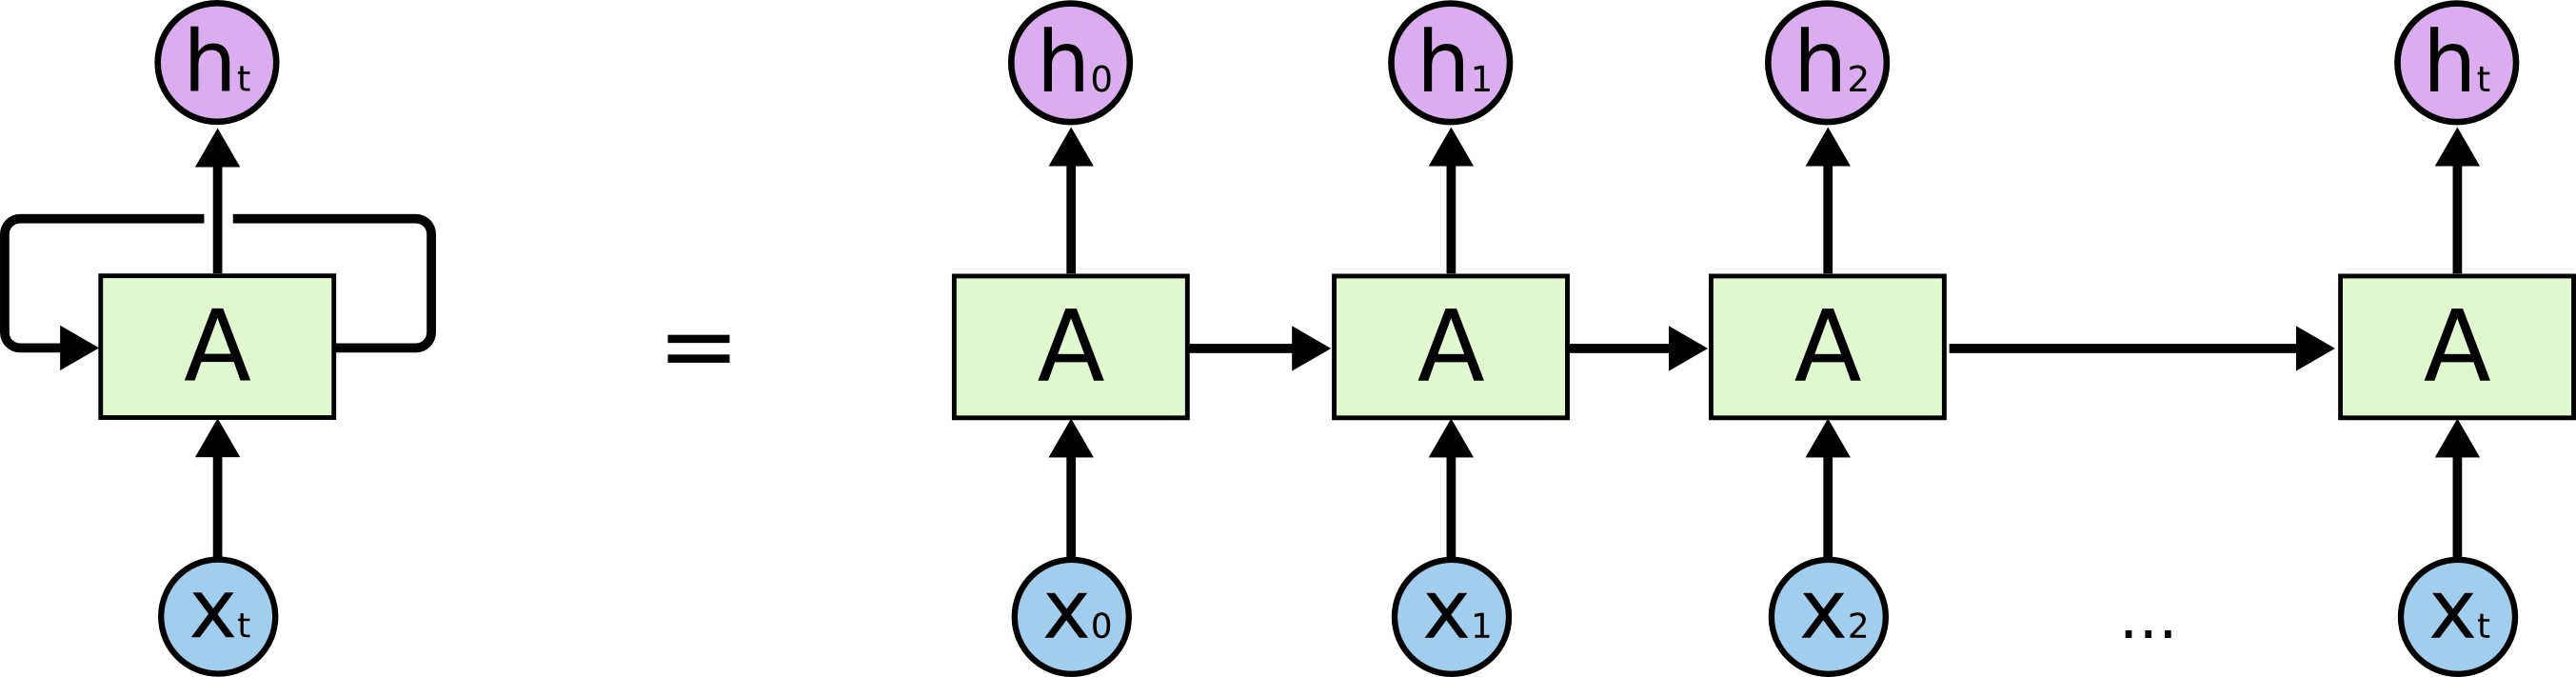
\includegraphics[width=\textwidth,height=\textheight,keepaspectratio]{Images/Theoretical basis/RNN-unrolled.png}
    \caption{Minh họa một mạng nơ-ron hồi quy}
    \label{fig:enter-label}
\end{figure}

\subsubsection{Một số loại mạng nơ-ron hồi quy}
\indent Mạng nơ-ron hồi quy (RNN) có thể được cấu hình theo nhiều cách khác nhau tùy thuộc vào loại bài toán cần giải quyết. Dưới đây là các dạng cấu trúc RNN phổ biến:
\begin{itemize}
    \item \textbf{Một-nhiều (One-to-Many):} Trong cấu hình này, từ một đầu vào duy nhất, mạng tạo ra một chuỗi các đầu ra. Loại này thường được ứng dụng trong các bài toán như tạo chú thích hình ảnh, nơi mạng nơ-ron tạo ra một câu hoàn chỉnh dựa trên một hình ảnh đầu vào duy nhất.
    \item \textbf{Nhiều-một (Many-to-One):} Đây là cấu trúc mà mạng nhận một chuỗi dữ liệu đầu vào và đưa ra một đầu ra duy nhất. Một ví dụ điển hình là phân tích cảm xúc, nơi RNN nhận một đoạn văn bản và dự đoán cảm xúc tổng quát (như tích cực, tiêu cực hoặc trung tính).
    \item \textbf{Nhiều-một (Many-to-Many):} Mạng này xử lý nhiều đầu vào và tạo ra nhiều đầu ra tương ứng. Đây là cấu trúc phổ biến trong các ứng dụng dịch máy, nơi mạng nhận một câu ở ngôn ngữ nguồn và chuyển đổi nó thành một câu tương ứng ở ngôn ngữ đích.
\end{itemize}

\begin{figure}[H]
    \centering
    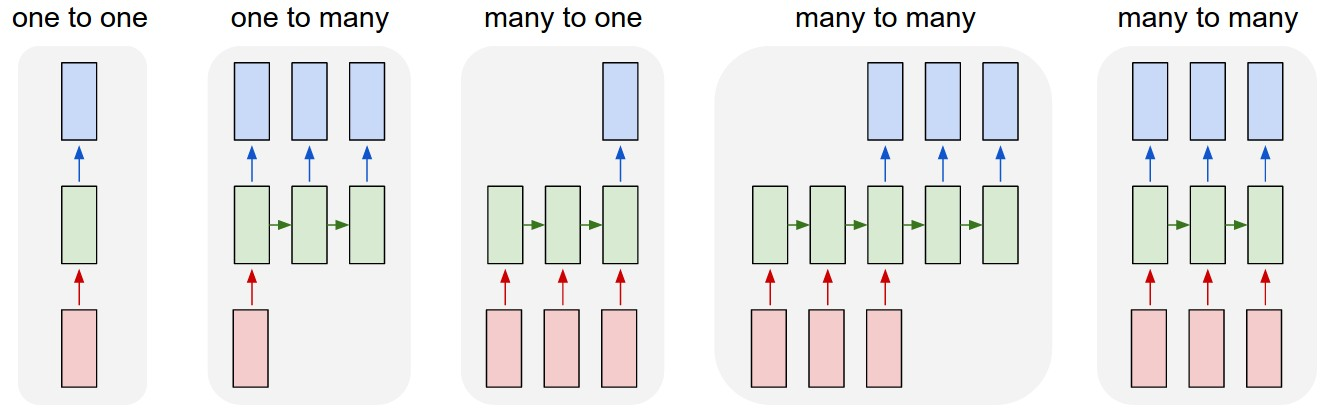
\includegraphics[width=\textwidth,height=\textheight,keepaspectratio]{Images/Theoretical basis/RNN_Type.jpeg}
    \caption{Một số kiểu nơ-ron hồi quy phổ biến}
    \label{fig:enter-label}
\end{figure}
\subsubsection{Vấn đề phụ thuộc xa của RNN}

\indent Một trong những đặc điểm nổi bật của mạng nơ-ron hồi quy (RNN) là khả năng tận dụng thông tin từ các bước trước trong chuỗi dữ liệu để dự đoán các bước tiếp theo. Điều này tương tự như cách con người sử dụng bối cảnh từ các đoạn văn trước để hiểu một đoạn văn hiện tại. Tuy nhiên, khả năng này của RNN không phải lúc nào cũng hiệu quả và còn phụ thuộc vào khoảng cách giữa thông tin cần thiết và thông tin hiện tại.

\indent Trong các trường hợp đơn giản, khi khoảng cách giữa dữ liệu cần ghi nhớ và thông tin hiện tại là ngắn, RNN có thể hoạt động tốt. Ví dụ, khi đọc câu "Các đám mây trên bầu trời...", thông tin về cụm từ "bầu" ngay lập tức gợi ý từ "trời". Đây là một dạng phụ thuộc ngắn hạn mà RNN có thể xử lý dễ dàng.
\begin{figure}[H]
    \centering
    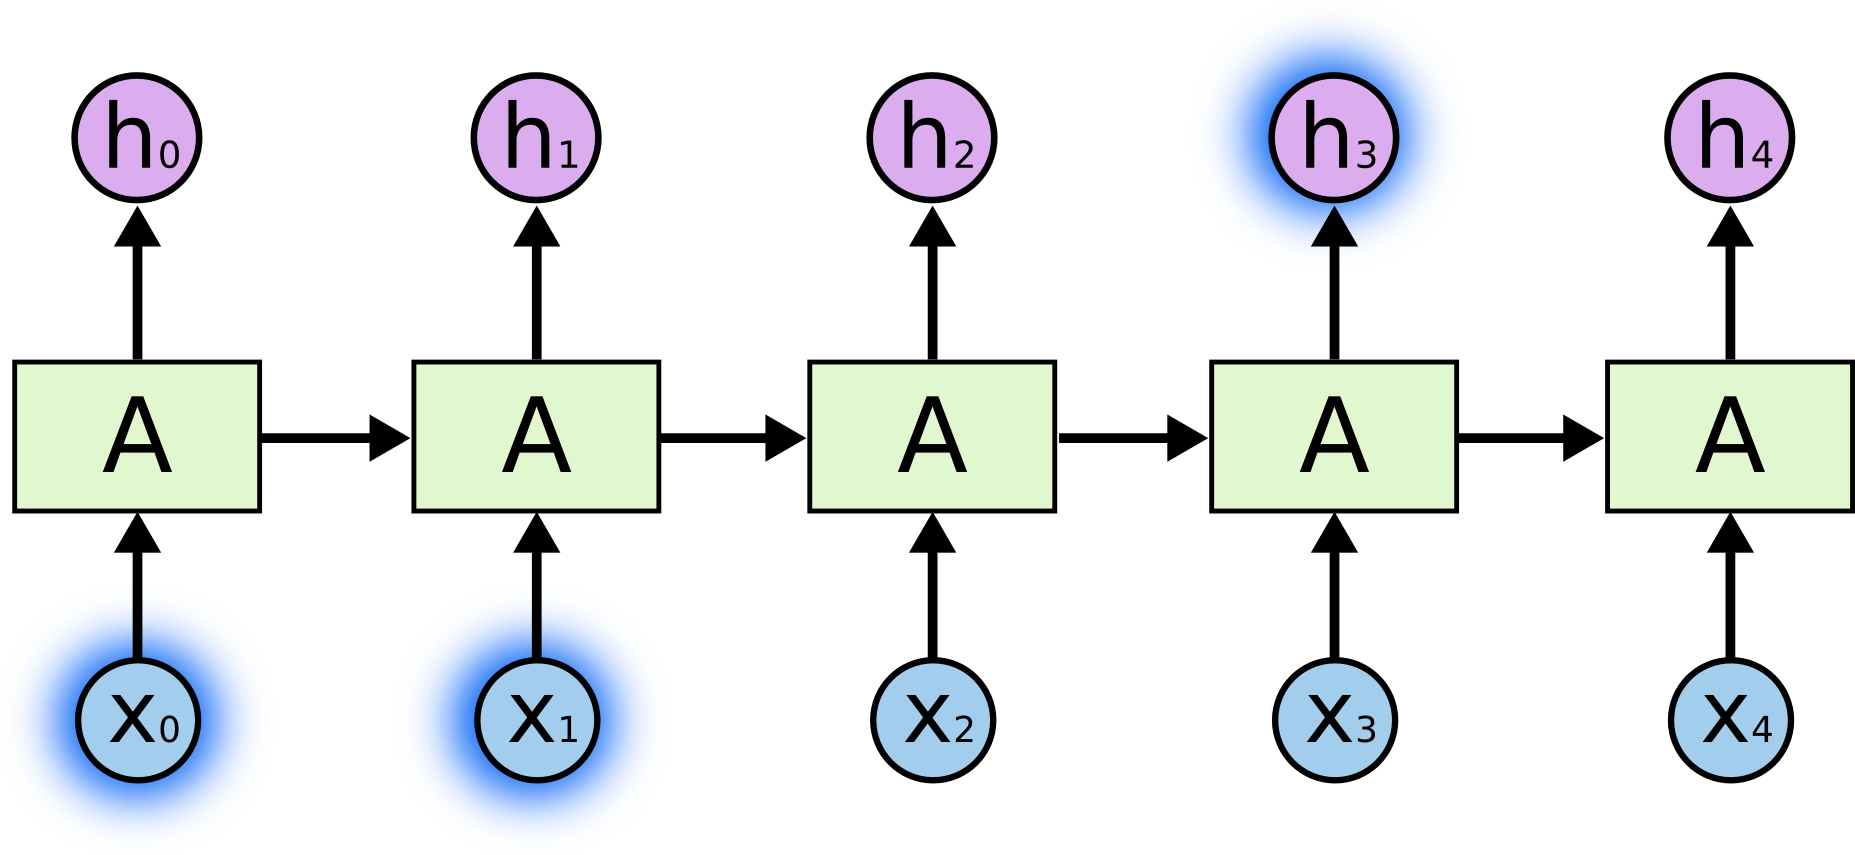
\includegraphics[width=\textwidth,height=\textheight,keepaspectratio]{Images/Theoretical basis/RNN-shorttermdepdencies.png}
    \caption{Phụ thuộc ngắn hạn trên RNN}
    \label{fig:enter-label}
\end{figure}
\indent Tuy nhiên, khi cần đến các mối quan hệ phức tạp hơn với khoảng cách xa, RNN bắt đầu gặp khó khăn. Chẳng hạn, trong câu "Tôi lớn lên ở Pháp... Tôi nói tiếng Pháp rất lưu loát", thông tin gần như "Tôi nói tiếng..." không đủ để xác định đó là ngôn ngữ nào. Việc suy luận đúng cần dựa vào thông tin ở câu trước đó, "Tôi lớn lên ở Pháp". Khi khoảng cách giữa dữ liệu cần nhớ và thông tin hiện tại tăng lên, RNN thường mất khả năng ghi nhớ và học hiệu quả.
\begin{figure}[H]
    \centering
    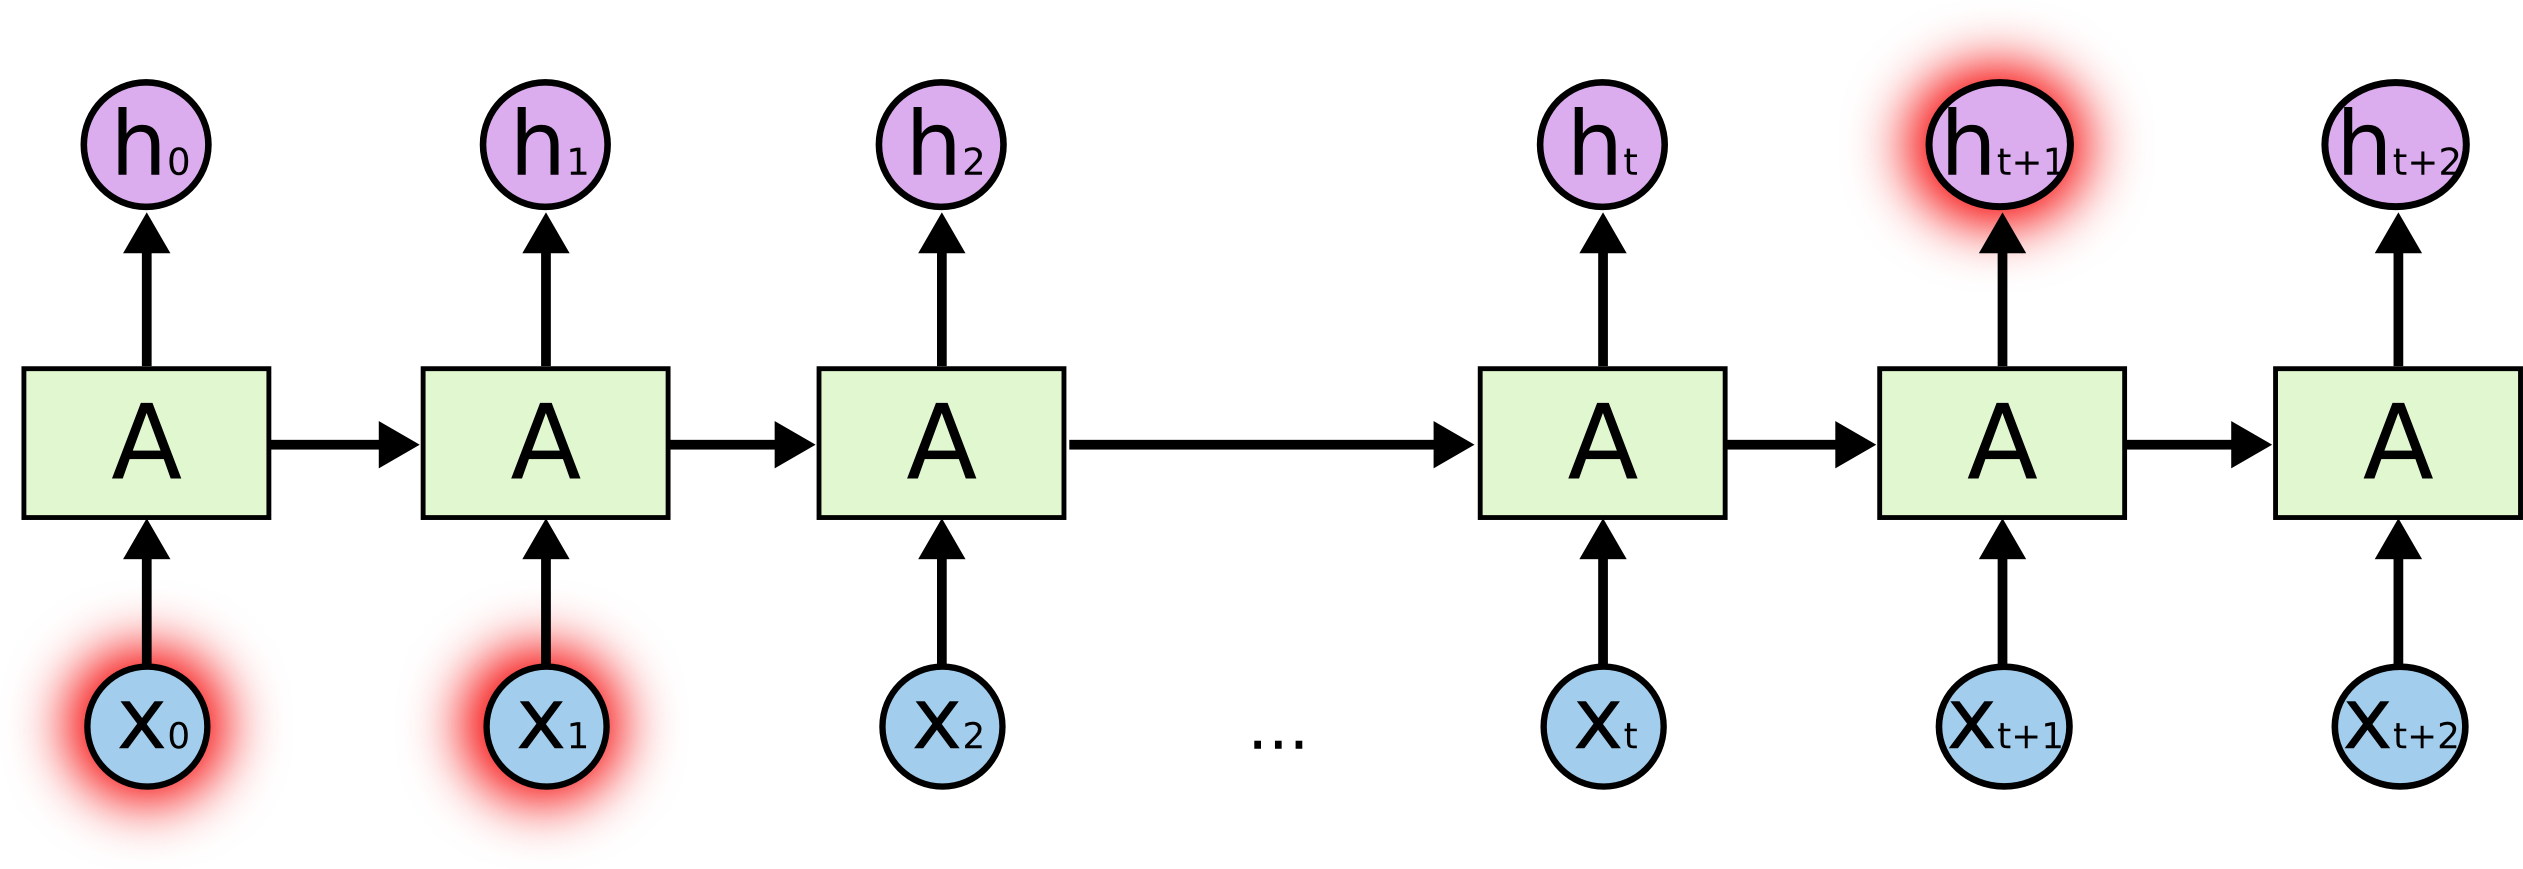
\includegraphics[width=\textwidth,height=\textheight,keepaspectratio]{Images/Theoretical basis/RNN-longtermdependencies.png}
    \caption{Phụ thuộc dài hạn trên RNN}
    \label{fig:enter-label}
\end{figure}
\indent Nguyên nhân chính là do hiện tượng triệt tiêu gradient (vanishing gradient), khiến cho các tín hiệu từ các bước trước đó bị yếu dần trong quá trình lan truyền ngược. Điều này khiến RNN không thể lưu giữ được thông tin dài hạn, gây ảnh hưởng nghiêm trọng đến hiệu quả xử lý của mạng.


\subsection{Giói thiệu mô hình Long-short term memmory(LTSM)}
\subsubsection{Giới thiệu tổng quan}

\indent Long Short-Term Memory (LSTM) là một loại mạng nơ-ron hồi quy (RNN) đặc biệt được thiết kế để giải quyết vấn đề phụ thuộc xa trong dữ liệu tuần tự. LSTM lần đầu tiên được giới thiệu bởi Hochreiter và Schmidhuber vào năm 1997 và sau đó đã được cải tiến bởi nhiều nhà nghiên cứu khác, giúp nó trở thành một công cụ quan trọng trong lĩnh vực học sâu.

\indent Khác với RNN truyền thống, LSTM có khả năng lưu trữ thông tin trong một khoảng thời gian dài hơn nhờ vào cấu trúc độc đáo với các cổng điều khiển thông minh. Những cổng này bao gồm cổng quên, cổng đầu vào và cổng đầu ra, cho phép mô hình lựa chọn giữ lại hay loại bỏ thông tin một cách có chọn lọc. Điều này giúp LSTM khắc phục được các hạn chế như triệt tiêu hoặc bùng nổ gradient, vốn là vấn đề phổ biến trong RNN tiêu chuẩn.

\indent LSTM hoạt động hiệu quả trên nhiều bài toán khác nhau, từ xử lý ngôn ngữ tự nhiên, dự đoán chuỗi thời gian đến nhận dạng giọng nói và video. Chính sự linh hoạt và khả năng xử lý dữ liệu tuần tự dài hạn này đã khiến LSTM trở thành một lựa chọn phổ biến trong các ứng dụng học sâu.

\begin{figure}[H]
    \centering
    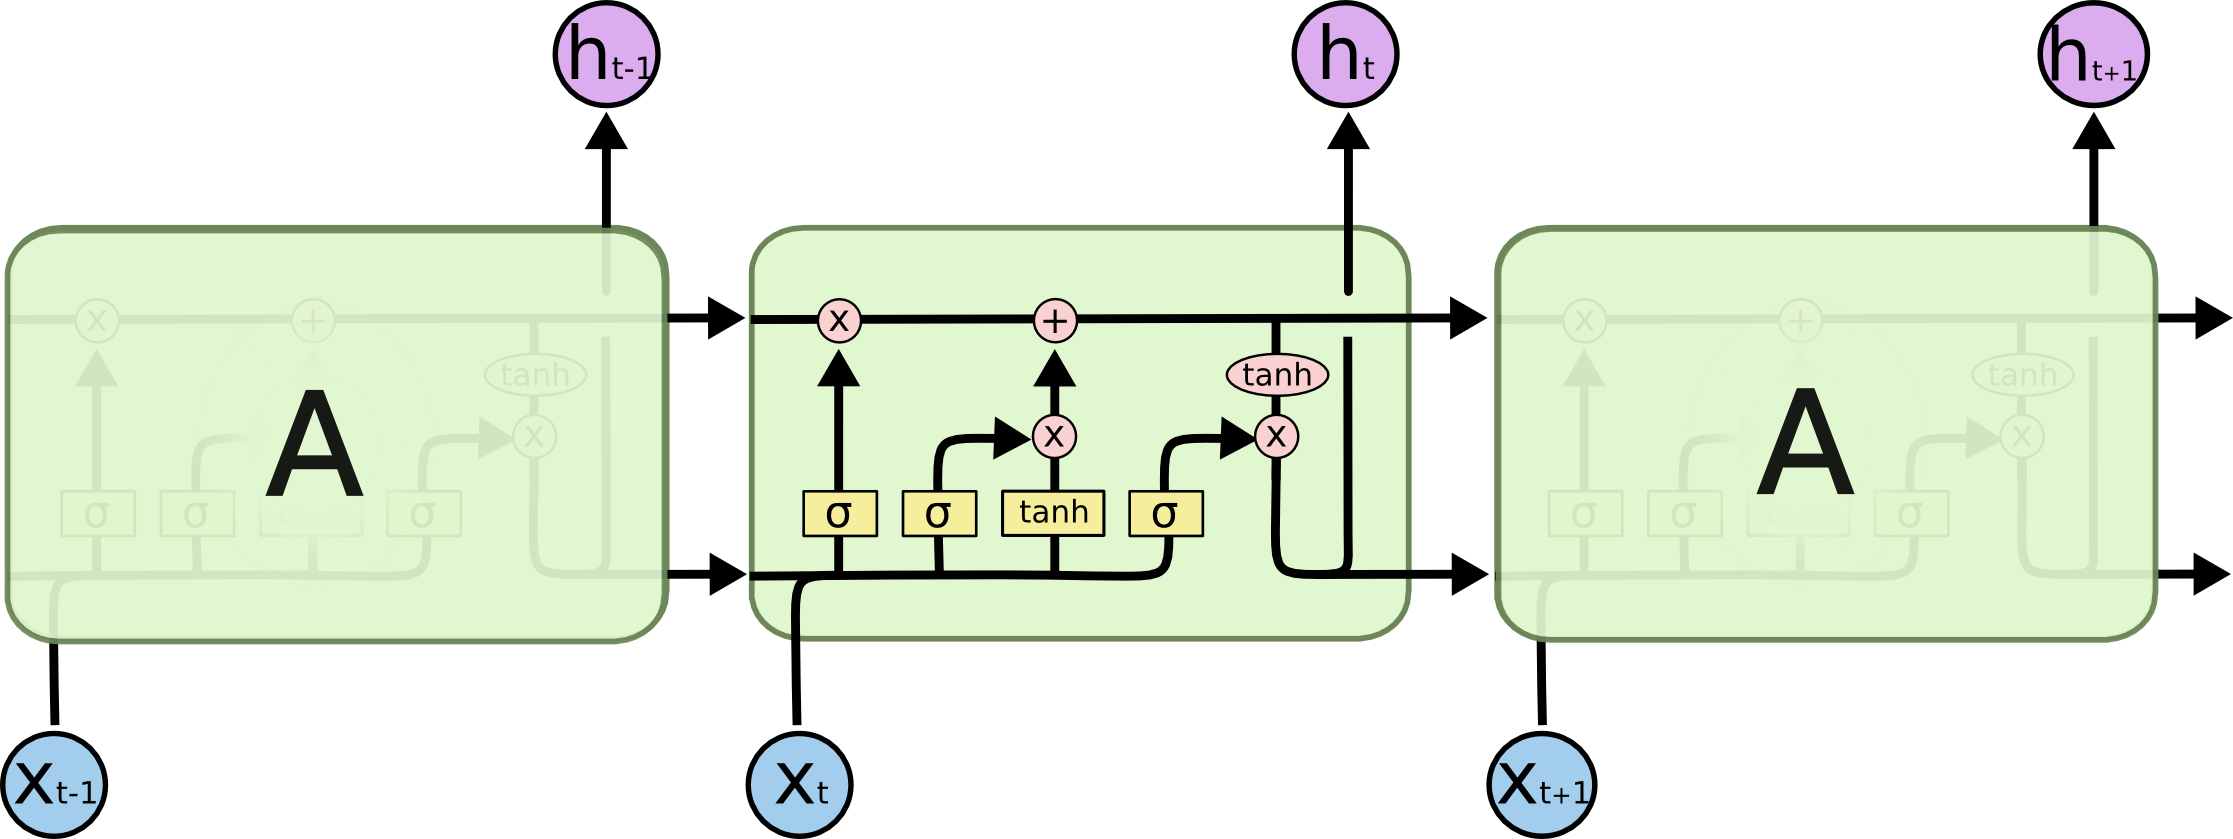
\includegraphics[width=14cm]{Images/Theoretical basis/LSTM.png}
\caption{Mô hình LSTM với 4 lớp tương tác}
\end{figure}
\subsubsection{Ý tưởng đằng sau LSTM}

\begin{figure}[H]
    \centering
    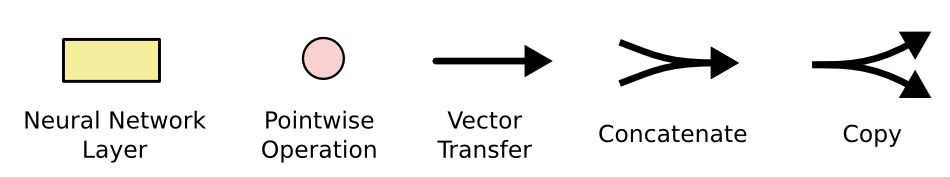
\includegraphics[width=14cm]{Images/Architecture/lstm1.png}
\caption{Diễn giải các kí hiệu trong đồ thị}
\end{figure}

\indent Mạng LSTM được thiết kế với mục đích giải quyết vấn đề phụ thuộc xa trong RNN bằng cách sử dụng một thành phần đặc biệt gọi là ô trạng thái (cell state). Ô trạng thái này hoạt động như một đường dẫn thẳng xuyên suốt chuỗi dữ liệu, giúp truyền tải thông tin mà không bị mất mát quá nhiều qua thời gian. Điều này giúp LSTM có thể nhớ được thông tin trong khoảng thời gian dài mà không gặp phải vấn đề triệt tiêu gradient.

\begin{itemize}
    \item Ô trạng thái (cell state) được thể hiện qua đường chạy ngang qua đỉnh đồ thị như hình vẽ bên dưới:
    \begin{figure}[H]
        \centering
        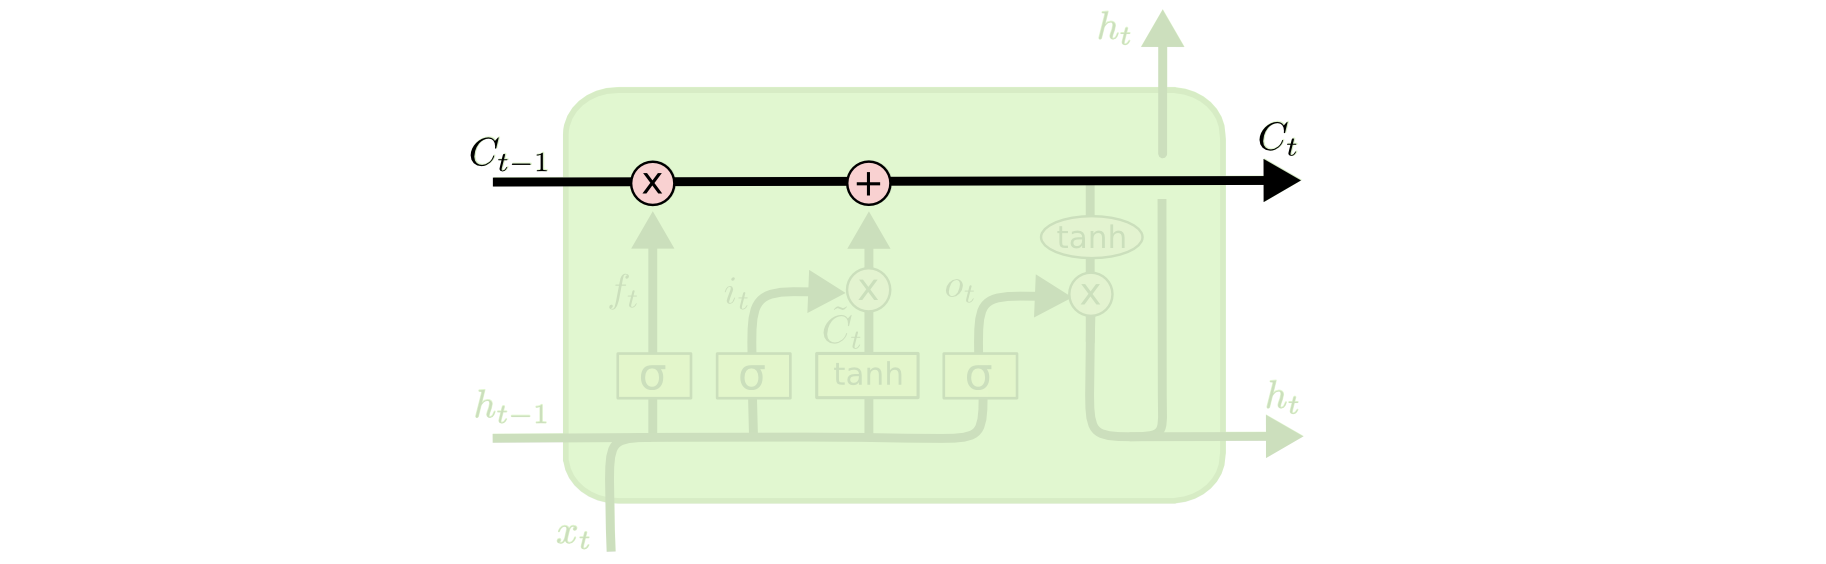
\includegraphics[width=14cm]{Images/Architecture/LSTM3-C-line.png}
    \caption{Đường đi của ô trạng thái (cell state) trong mạng LSTM}
    \end{figure}
    \item Ô trạng thái là một dạng băng chuyền chạy thẳng xuyên suốt toàn bộ chuỗi với chỉ một vài tương tác tuyến tính nhỏ giúp cho thông tin có thể truyền dọc theo đồ thị mạng nơ-ron ổn định.
    \item LSTM có khả năng xóa và thêm thông tin vào ô trạng thái và điều chỉnh các luồng thông tin này thông qua các cấu trúc gọi là cổng.
    \item Cổng là cơ chế đặc biệt để điều chỉnh luồng thông tin đi qua. Chúng được tổng hợp bởi một tầng ẩn của hàm activation sigmoid và với một toán tử nhân như đồ thị.
    \begin{figure}[H]
        \centering
        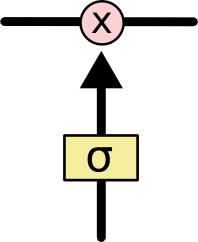
\includegraphics[width=3cm]{Images/Architecture/LSTM3-gate.png}
    \caption{Một cổng của hàm sigmoid trong LSTM}
    \end{figure}
    \item Hàm sigmoid sẽ cho đầu ra là một giá trị xác xuất nằm trong khoảng từ 0 đến 1, thể hiện rằng có bao nhiêu phần thông tin sẽ đi qua cổng. Giá trị bằng 0 ngụ ý rằng không cho phép thông tin nào đi qua, giá trị bằng 1 sẽ cho toàn bộ thông tin đi qua.
    \item Một mạng LSTM sẽ có 3 cổng có kiến trúc dạng này để bảo vệ và kiểm soát các ô trạng thái.
\end{itemize}

\subsubsection{Thứ tự các bước của LSTM}

\indent Bước đầu tiên trong LSTM sẽ quyết định xem thông tin nào chúng ta sẽ cho phép đi qua ô trạng thái (cell state). Nó được kiểm soát bởi hàm sigmoid trong một tầng gọi là tầng quên (forget gate layer). Đầu tiên nó nhận đầu vào là 2 giá trị \( h_{t-1} \)
 và \( x_{t} \)
 và trả về một giá trị nằm trong khoảng 0 và 1 cho mỗi giá trị của ô trạng thái \( \text{C}_{t-1} \)
. Nếu giá trị bằng 1 thể hiện ‘giữ toàn bộ thông tin’ và bằng 0 thể hiện ‘bỏ qua toàn bộ chúng’.

\indent Trở lại ví dụ về ngôn ngữ, chúng ta đang cố gắng dự báo từ tiếp theo dựa trên toàn bộ những từ trước đó. Trong những bài toán như vậy, ô trạng thái có thể bao gồm loại của chủ ngữ hiện tại, để cho đại từ ở câu tiếp theo được sử dụng chính xác. Chẳng hạn như chúng ta đang mô tả về một người bạn là con trai thì các đại từ nhân xưng ở tiếp theo phải là anh, thằng, hắn thay vì cô, con ấy. Tuy nhiên chủ ngữ không phải khi nào cũng cố định. Khi chúng ta nhìn thấy một chủ ngữ mới, chúng ta muốn quên đi loại của một chủ ngữ cũ. Do đó tầng quên cho phép cập nhật thông tin mới và lưu giữ giá trị của nó khi có thay đổi theo thời gian.

\begin{figure}[H]
    \centering
    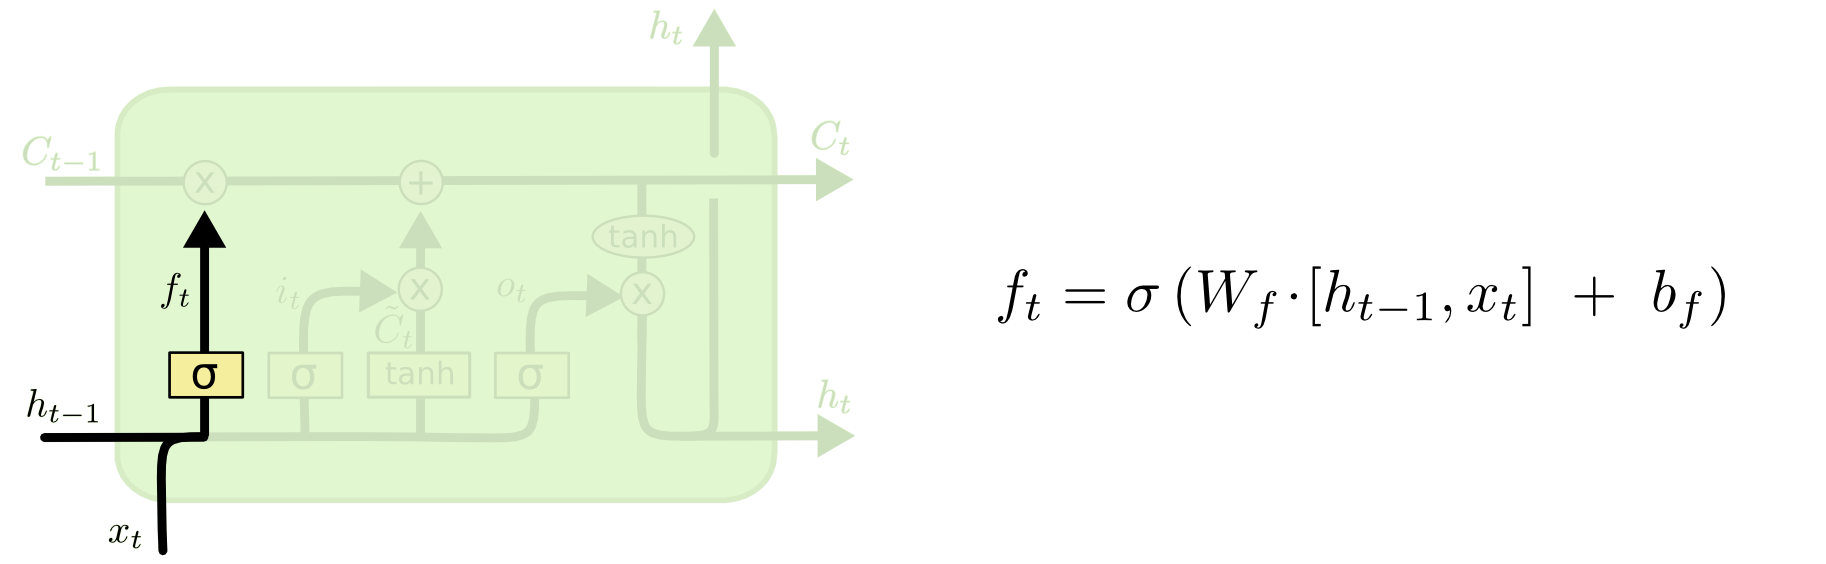
\includegraphics[width=14cm]{Images/Architecture/LSTM3-focus-f.png}
\caption{Tầng cổng quên (forget gate layer)}
\end{figure}

\indent Bước tiếp theo chúng ta sẽ quyết định loại thông tin nào sẽ được lưu trữ trong ô trạng thái. Bước này bao gồm 2 phần. Phần đầu tiên là một tầng ẩn của hàm sigmoid được gọi là tầng cổng vào (input gate layer) quyết định giá trị bao nhiêu sẽ được cập nhật. Tiếp theo, tầng ẩn hàm tanh sẽ tạo ra một véc tơ của một giá trị trạng thái mới 
 mà có thể được thêm vào trạng thái. Tiếp theo kết hợp kết quả của 2 tầng này để tạo thành một cập nhật cho trạng thái.

\indent Trong ví dụ của mô hình ngôn ngữ, chúng ta muốn thêm loại của một chủ ngữ mới vào ô trạng thái để thay thế phần trạng thái cũ muốn quên đi.

\begin{figure}[H]
    \centering
    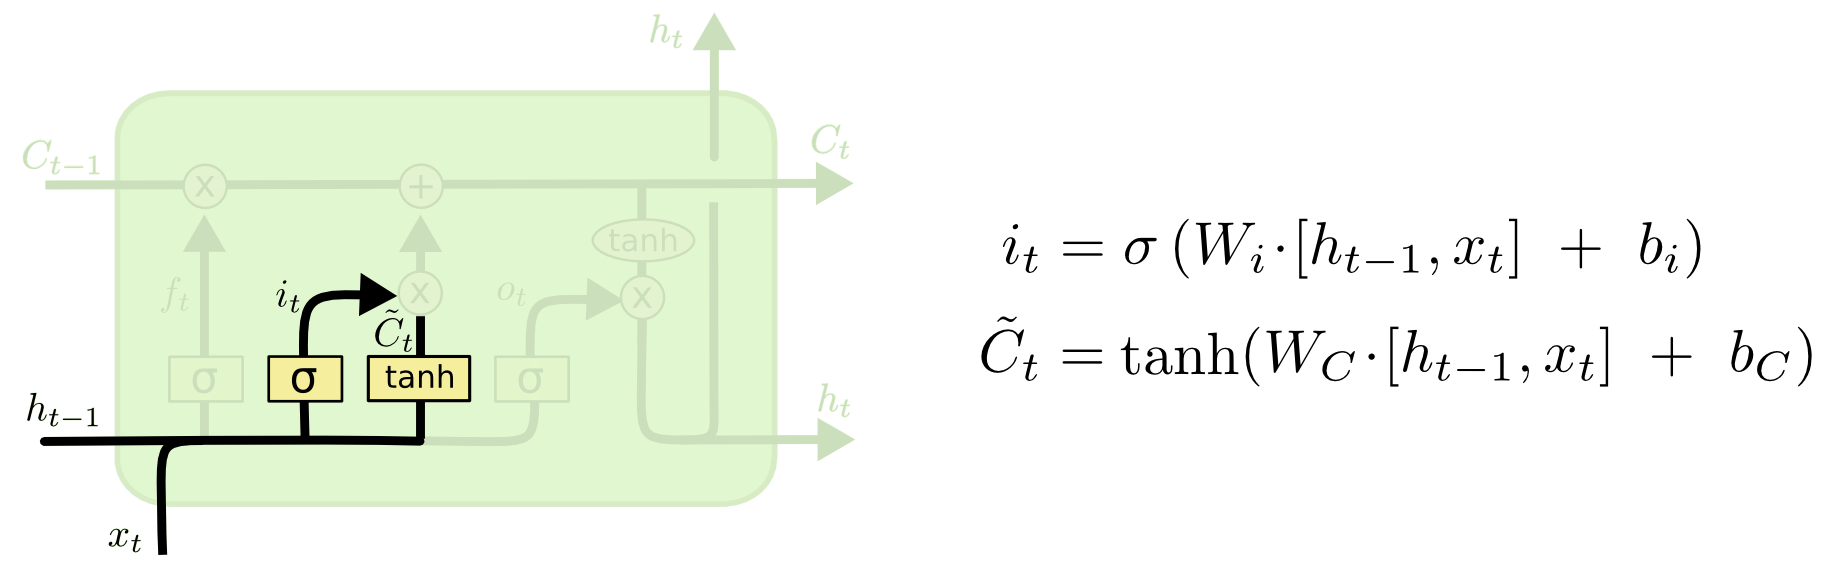
\includegraphics[width=14cm]{Images/Architecture/LSTM3-focus-i.png}
\caption{ Cập nhật giá trị cho ô trạng thái bằng cách kết hợp 2 kết quả từ tầng cổng vào và tẩng ẩn hàm tanh}
\end{figure}

\indent Đây là thời điểm để cập nhật một ô trạng thái cũ \( \text{C}_{t-1} \)
 sang một trạng thái mới \( \text{C}_{t} \)
. Những bước trước đó đã quyết định làm cái gì, và tại bước này chỉ cần thực hiện nó.

\indent Chúng ta nhân trạng thái cũ với \( f_{t} \)
 tương ứng với việc quên những thứ quyết định được phép quên sớm. Phần tử đề cử \( \tilde{\text{C}}_{t-1} \)
 là một giá trị mới được tính toán tương ứng với bao nhiêu được cập nhật vào mỗi giá trị trạng thái.

 \begin{figure}[H]
    \centering
    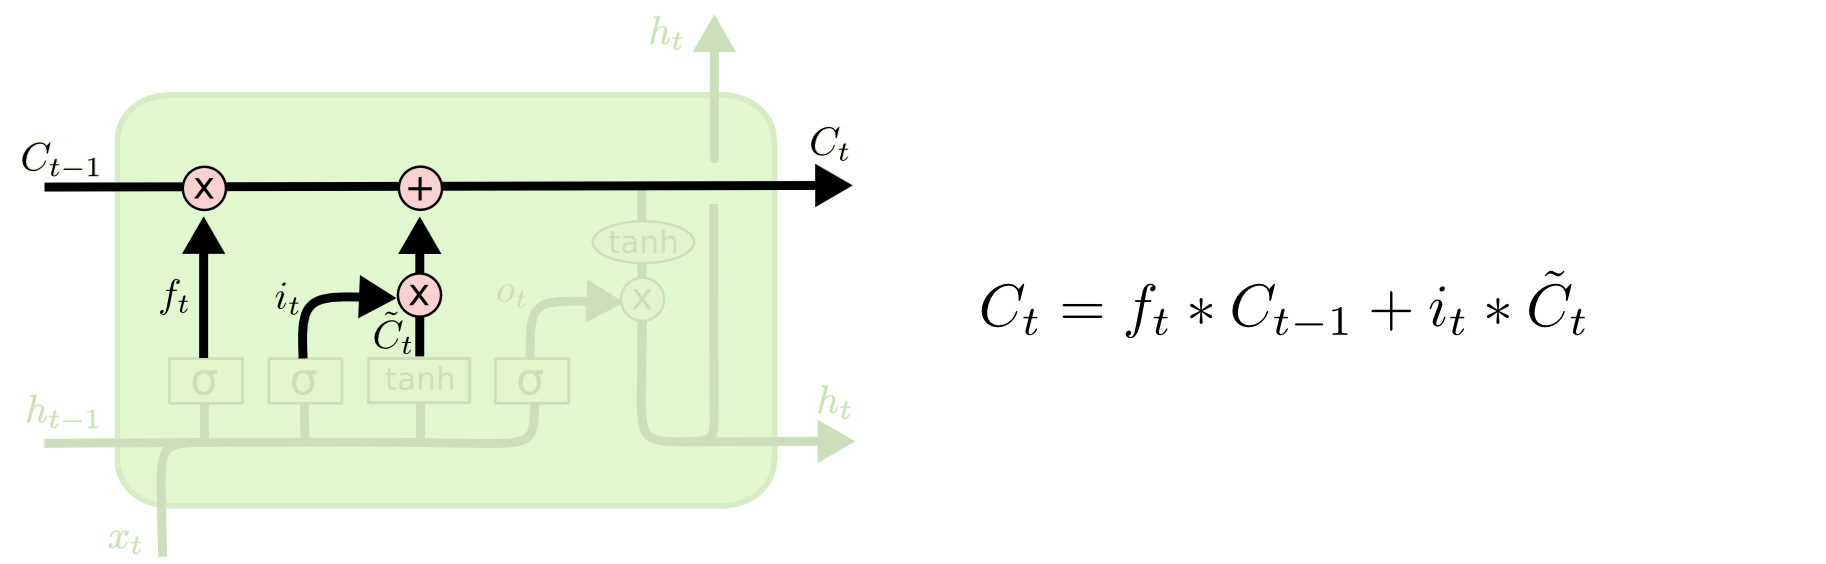
\includegraphics[width=14cm]{Images/Architecture/LSTM3-focus-C.png}
\caption{Ô trạng thái mới}
\end{figure}

\indent Cuối cùng cần quyết định xem đầu ra sẽ trả về bao nhiêu. Kết quả ở đầu ra sẽ dựa trên ô trạng thái, nhưng sẽ là một phiên bản được lọc. Đầu tiên, chúng ta chạy qua một tầng sigmoid nơi quyết định phần nào của ô trạng thái sẽ ở đầu ra. Sau đó, ô trạng thái được đưa qua hàm tanh (để chuyển giá trị về khoảng -1 và 1) và nhân nó với đầu ra của một cổng sigmoid, do đó chỉ trả ra phần mà chúng ta quyết định.

 \begin{figure}[H]
    \centering
    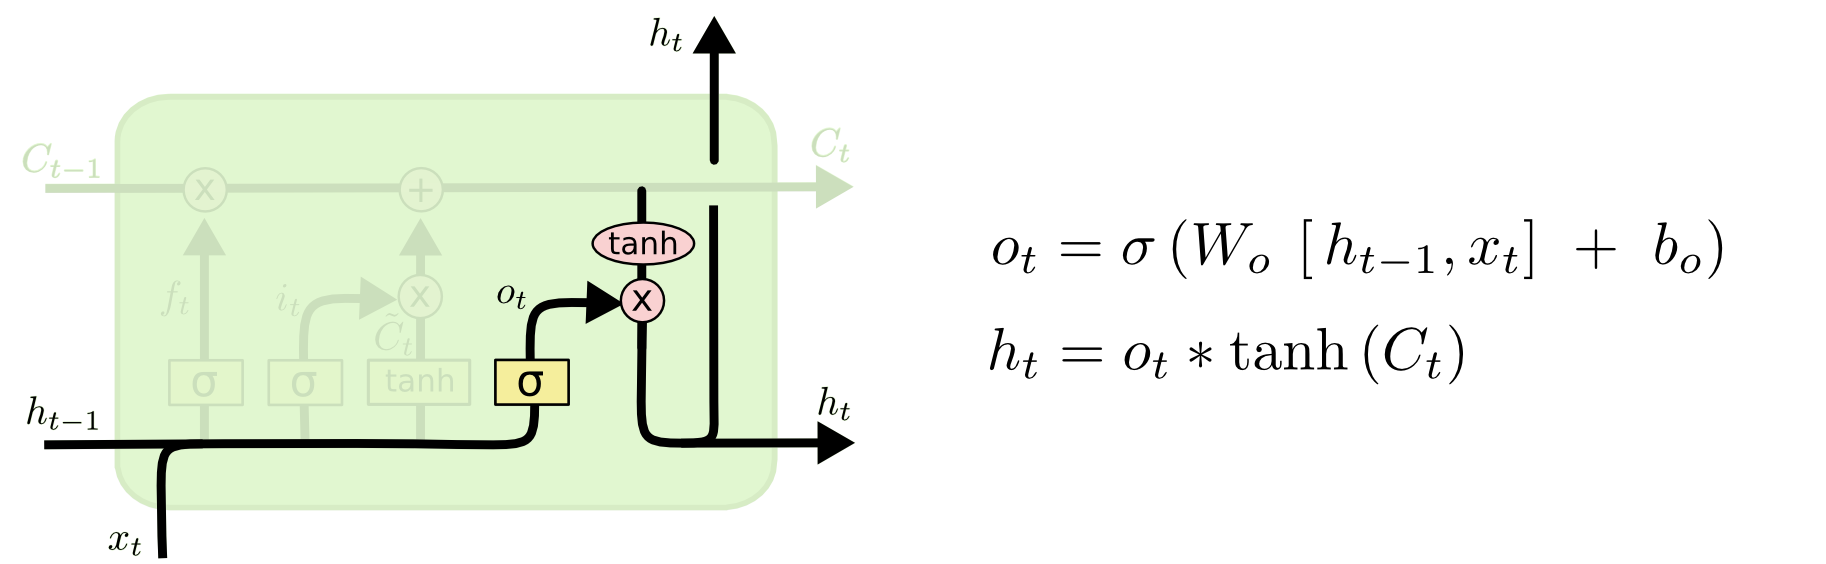
\includegraphics[width=14cm]{Images/Architecture/LSTM3-focus-o.png}
\caption{Điều chỉnh thông tin ở đầu ra thông qua hàm tanh}
\end{figure}
\subsubsection{Ưu và nhược điểm của mô hình LSTM}

\textbf{Ưu điểm}
\begin{itemize}
    \item LSTM được thiết kế đặc biệt để giải quyết vấn đề phụ thuộc dài hạn trong dữ liệu tuần tự. Nhờ vào ô trạng thái và cơ chế các cổng, LSTM có khả năng lưu trữ thông tin trong thời gian dài mà không bị mất mát như các mạng RNN truyền thống.
    \item LSTM có thể học và theo dõi các mối quan hệ phức tạp giữa các phần tử trong chuỗi dữ liệu dài, giúp giải quyết các bài toán như dịch ngôn ngữ, nhận diện giọng nói và phân tích chuỗi thời gian.
    \item Các cổng trong LSTM giúp giảm thiểu vấn đề triệt tiêu gradient, mà thường gặp phải trong các mạng RNN thông thường. Điều này cho phép mạng có thể học được thông tin từ các bước thời gian xa mà không gặp phải sự giảm sút mạnh mẽ của gradient.
    \item LSTM có thể được sử dụng trong nhiều bài toán khác nhau và có thể kết hợp với các mô hình học sâu phức tạp để tạo thành các mạng học sâu đa lớp, linh hoạt và hiệu quả trong việc xử lý các loại dữ liệu khác nhau.
\end{itemize}
\textbf{Nhược điểm}
\begin{itemize}
    \item LSTM có cấu trúc phức tạp hơn so với các mạng nơ-ron hồi quy thông thường. Việc tính toán và tối ưu các tham số trong LSTM yêu cầu tài nguyên tính toán lớn và thời gian huấn luyện dài, đặc biệt là với các mô hình có số lớp lớn và dữ liệu phức tạp.
    \item Do tính toán phức tạp và yêu cầu số lượng tham số lớn, quá trình huấn luyện mô hình LSTM có thể mất nhiều thời gian, đặc biệt là khi làm việc với bộ dữ liệu lớn.
    \item LSTM dễ gặp phải vấn đề overfitting, đặc biệt là khi sử dụng với bộ dữ liệu huấn luyện nhỏ hoặc khi mạng quá phức tạp. Điều này có thể dẫn đến việc mô hình học quá chi tiết từ dữ liệu huấn luyện mà không có khả năng tổng quát tốt trên dữ liệu mới.
    \item Mặc dù LSTM giải quyết được vấn đề triệt tiêu gradient, nhưng vấn đề gradient exploding (gradient phát triển quá mức) vẫn có thể xảy ra. Điều này có thể làm mô hình trở nên không ổn định, đặc biệt trong quá trình huấn luyện với các chuỗi dữ liệu rất dài.
\end{itemize}

\subsection{Giới thiệu về Transfer Learning}

Transfer learning (học chuyển giao) là một kỹ thuật học máy trong đó một mô hình được phát triển cho một nhiệm vụ được sử dụng lại như là điểm khởi đầu cho một mô hình trên một nhiệm vụ thứ hai. Nói cách khác, kiến thức thu được trong khi giải quyết một vấn đề được áp dụng cho một vấn đề khác, nhưng có liên quan. 

\subsubsection{Định nghĩa Transfer Learning}

Transfer learning là việc sử dụng kiến thức đã học từ một miền nguồn (source domain) để cải thiện việc học trong một miền đích (target domain) khác. Miền nguồn thường có lượng dữ liệu lớn hơn và/hoặc dễ học hơn miền đích. 

 \begin{figure}[H]
    \centering
    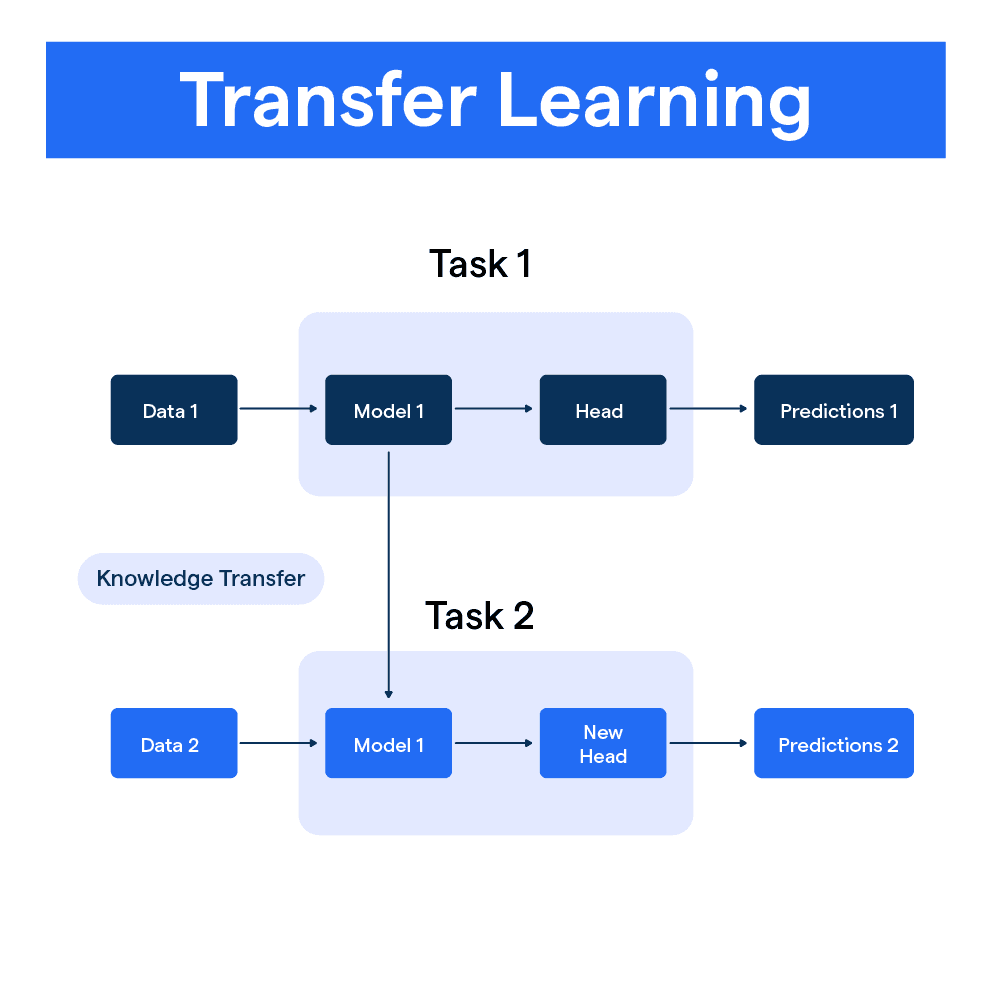
\includegraphics[width=10cm]{Images/Theoretical basis/Transfer_Learning.png}
\caption{Transfer learning}
\end{figure}


\subsubsection{Ứng dụng của Transfer Learning}

Transfer learning đã được ứng dụng thành công trong nhiều lĩnh vực, bao gồm:

\begin{itemize}
    \item \textbf{Thị giác máy tính:} 
        \begin{itemize}
            \item Phân loại ảnh: Xác định các đối tượng trong ảnh (chó, mèo, xe hơi,...)
            \item Nhận dạng đối tượng: Xác định vị trí của các đối tượng trong ảnh.
            \item Phân đoạn ảnh: Phân chia ảnh thành các vùng có ý nghĩa.
        \end{itemize}
    \item \textbf{Xử lý ngôn ngữ tự nhiên:}
        \begin{itemize}
            \item Phân loại văn bản: Phân loại các tài liệu văn bản (tin tức, đánh giá,...)
            \item Phân tích cảm xúc: Xác định cảm xúc được thể hiện trong văn bản.
            \item Dịch máy: Dịch văn bản từ ngôn ngữ này sang ngôn ngữ khác.
        \end{itemize}
    \item \textbf{Âm thanh và lời nói:}
        \begin{itemize}
            \item Nhận dạng giọng nói: Chuyển đổi lời nói thành văn bản.
            \item Tổng hợp giọng nói: Tạo ra giọng nói từ văn bản.
        \end{itemize}
\end{itemize}

\subsubsection{Lợi ích và bất lợi của Transfer Learning}

\textbf{Lợi ích:}

 \begin{figure}[H]
    \centering
    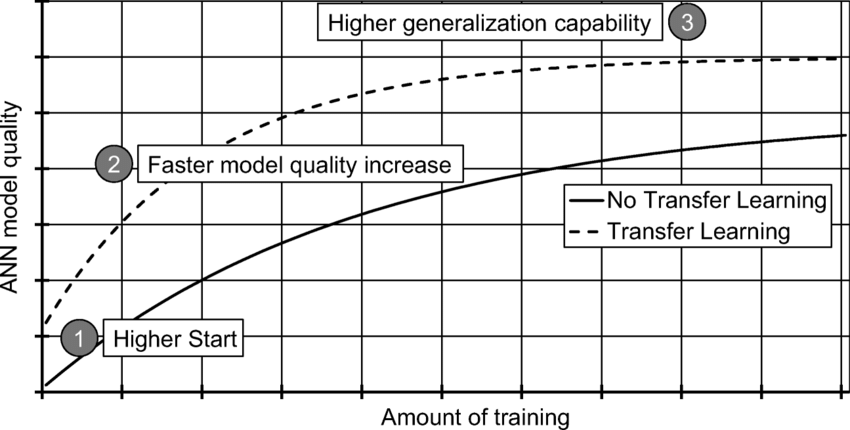
\includegraphics[scale = 0.4]{Images/Theoretical basis/Possible-advantages-of-transfer-learning.png}
\caption{Lợi ích của Transfer Learning}
\end{figure}


\begin{itemize}
    \item Cải thiện hiệu suất của mô hình, đặc biệt là khi dữ liệu huấn luyện hạn chế.
    \item Giảm thời gian huấn luyện và tài nguyên tính toán.
    \item Nâng cao khả năng khái quát hóa của mô hình.
\end{itemize}

\textbf{Bất lợi:}

\begin{itemize}
    \item Có thể xảy ra hiện tượng "negative transfer" nếu miền nguồn và miền đích quá khác biệt.
    \item Khó khăn trong việc lựa chọn mô hình tiền huấn luyện phù hợp.
\end{itemize}
\subsection{Giới thiệu về Self-Attention}

Self-attention là một cơ chế trong học sâu cho phép mô hình tập trung vào các phần khác nhau của dữ liệu đầu vào khi xử lý nó. Nó đã trở thành một thành phần quan trọng trong nhiều kiến trúc mạng nơ-ron hiện đại, đặc biệt là trong lĩnh vực xử lý ngôn ngữ tự nhiên.

\subsubsection{Cơ chế hoạt động của Self-Attention}

Self-attention hoạt động bằng cách tính toán mối quan hệ giữa các phần tử khác nhau trong một chuỗi. Mỗi phần tử được biểu diễn bằng một vector, và self-attention tính toán "attention weights" (trọng số chú ý) để xác định mức độ quan trọng của mỗi phần tử đối với các phần tử khác. Các trọng số này sau đó được sử dụng để tạo ra một biểu diễn mới cho mỗi phần tử, kết hợp thông tin từ các phần tử liên quan.


 \begin{figure}[H]
    \centering
    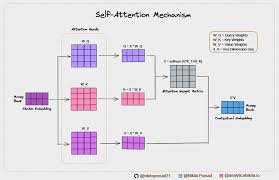
\includegraphics[scale = 1]{Images/Theoretical basis/self-attention.jpg}
\caption{Self Attention}
\end{figure}

\subsubsection{Các loại Self-Attention thường gặp}

Có nhiều biến thể của self-attention, mỗi biến thể có những đặc điểm và ứng dụng riêng:

\begin{itemize}
    \item \textbf{Scaled Dot-Product Attention:} Đây là biến thể phổ biến nhất, được sử dụng trong Transformer. Nó tính toán attention weights dựa trên tích vô hướng của các vector biểu diễn.
    \item \textbf{Multi-Head Attention:}  Biến thể này sử dụng nhiều "head" attention song song, mỗi head tập trung vào các khía cạnh khác nhau của dữ liệu.
    \item \textbf{Additive Attention:} Biến thể này sử dụng một mạng nơ-ron để tính toán attention weights.
\end{itemize}

\subsubsection{Ứng dụng của Self-Attention}

Self-attention đã được ứng dụng rộng rãi trong nhiều lĩnh vực:

\begin{itemize}
    \item \textbf{Xử lý ngôn ngữ tự nhiên:} 
    \begin{itemize}
        \item Dịch máy
        \item Tóm tắt văn bản
        \item Phân tích cảm xúc
        \item Hỏi đáp
    \end{itemize}
    \item \textbf{Thị giác máy tính:}
    \begin{itemize}
        \item Phân loại ảnh
        \item Nhận dạng đối tượng
    \end{itemize}
    \item \textbf{Các lĩnh vực khác:}
    \begin{itemize}
        \item Sinh học
        \item Âm nhạc
    \end{itemize}
\end{itemize}

\subsubsection{Lợi ích của Self-Attention}

\begin{itemize}
    \item \textbf{Nắm bắt được các phụ thuộc dài hạn:} Self-attention có thể nắm bắt được mối quan hệ giữa các phần tử cách xa nhau trong chuỗi, điều mà các mô hình RNN truyền thống gặp khó khăn.
    \item \textbf{Tính toán song song hiệu quả:} Self-attention có thể được tính toán song song, giúp tăng tốc độ huấn luyện và suy luận.
    \item \textbf{Khả năng diễn giải tốt:} Attention weights cung cấp thông tin về các phần tử quan trọng trong chuỗi, giúp hiểu rõ hơn cách mô hình đưa ra quyết định.
\end{itemize}

\subsection{Nội suy tuyến tính (Linear Interpolation)}

\begin{figure}[H]
    \centering
    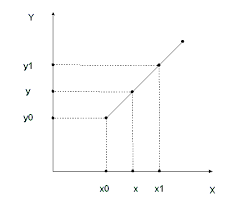
\includegraphics[scale = 1]{Images/Theoretical basis/linear_interpolation.png}
    \caption{Nội suy tuyến tính}    
\end{figure}

Nội suy tuyến tính là một phương pháp ước tính giá trị của một hàm số tại một điểm chưa biết, dựa trên giá trị của hàm số tại hai điểm đã biết. 

Giả sử ta có hai điểm dữ liệu $(x_1, y_1)$ và $(x_2, y_2)$, và ta muốn ước tính giá trị của hàm số $y = f(x)$ tại điểm $x$ nằm giữa $x_1$ và $x_2$. Nội suy tuyến tính giả định rằng hàm số $f(x)$ là một đường thẳng giữa hai điểm đã biết. 

Công thức nội suy tuyến tính được cho bởi:

$y = y_1 + \frac{(x - x_1)}{(x_2 - x_1)}(y_2 - y_1)$

Trong lĩnh vực học máy, nội suy tuyến tính thường được sử dụng để tạo ra các điểm dữ liệu mới từ tập dữ liệu hiện có. Ví dụ, trong bài toán xử lý ảnh, nội suy tuyến tính có thể được sử dụng để phóng to hoặc thu nhỏ ảnh. 

\subsubsection{Lợi ích của nội suy tuyến tính}
\begin{itemize}
    \item \textbf{Đơn giản:} Nội suy tuyến tính là một phương pháp đơn giản và dễ hiểu để ước lượng giá trị của một hàm số tại một điểm chưa biết.
\end{itemize}

\subsubsection{Hạn chế của nội suy tuyến tính}
\begin{itemize}
    \item \textbf{Giả định tuyến tính:} Nội suy tuyến tính giả định rằng hàm số là một đường thẳng giữa hai điểm đã biết, điều này có thể không phản ánh đúng mối quan hệ giữa các điểm dữ liệu.
\end{itemize}

\subsection{Generative Adversarial Networks (GANs)}

Generative Adversarial Networks (GANs) là một lớp mô hình học sâu mạnh mẽ được sử dụng để tạo ra dữ liệu mới, giống với dữ liệu huấn luyện. GANs bao gồm hai thành phần chính: generator và discriminator, hoạt động theo một cách đối kháng - generator cố gắng sinh dữ liệu sao cho giống với dữ liệu thật nhất, discriminator cố gắng phân biệt giữa dữ liệu sinh ra và dữ liệu thật cho đến khi discrimator không thể phân biệt được nữa.

 \begin{figure}[H]
    \centering
    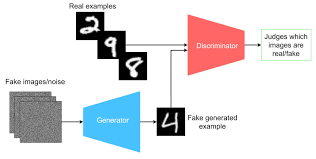
\includegraphics[scale = 0.8]{Images/Theoretical basis/GAN.png}
\caption{Generative Adversarial Networks (GANs)}
\end{figure}

\subsubsection{Kiến trúc và hoạt động của GANs}

\begin{itemize}
    \item \textbf{Generator:} Mạng nơ-ron này nhận vào một vector nhiễu ngẫu nhiên và cố gắng tạo ra dữ liệu giả mạo giống với dữ liệu thật.
    \item \textbf{Discriminator:} Mạng nơ-ron này nhận vào dữ liệu (thật hoặc giả mạo) và cố gắng phân biệt giữa chúng.
\end{itemize}
Hai mạng này được huấn luyện đồng thời: generator cố gắng đánh lừa discriminator, trong khi discriminator cố gắng không bị đánh lừa. Quá trình huấn luyện này tạo ra một vòng lặp phản hồi, trong đó cả hai mạng đều cải thiện theo thời gian.

\subsubsection{Các biến thể của GANs}

Có nhiều biến thể của GANs, mỗi biến thể có những đặc điểm và ứng dụng riêng:

\begin{itemize}
    \item \textbf{Deep Convolutional GANs (DCGANs):} Sử dụng mạng nơ-ron tích chập để tạo ra hình ảnh chất lượng cao.
    \item \textbf{Conditional GANs (cGANs):} Cho phép điều khiển quá trình tạo dữ liệu bằng cách cung cấp thông tin bổ sung (như nhãn lớp).
    \item \textbf{CycleGANs:} Cho phép chuyển đổi dữ liệu từ miền này sang miền khác (ví dụ: chuyển đổi ảnh từ mùa hè sang mùa đông).
    \item \textbf{Progressive Growing of GANs (PGGANs):}  Tạo ra hình ảnh có độ phân giải cao bằng cách tăng dần kích thước của mạng generator và discriminator.
    \item \textbf{StyleGAN:} Tạo ra hình ảnh chân thực với khả năng kiểm soát các thuộc tính tinh tế.
    \item \textbf{TimeGAN:} Tạo ra dữ liễu chuỗi thời gian mẫu từ tập dữ liệu đầu vào cho sẵn
\end{itemize}

\subsubsection{Ứng dụng của GANs}

GANs đã được ứng dụng trong nhiều lĩnh vực:

\begin{itemize}
    \item \textbf{Tạo hình ảnh:} Tạo ra hình ảnh chân thực của người, vật thể, cảnh quan,...
    \item \textbf{Tạo dữ liệu:} Tạo ra dữ liệu tổng hợp cho các tác vụ học máy khác.
    \item \textbf{Chỉnh sửa ảnh:}  Thay đổi các thuộc tính của ảnh (ví dụ: thêm nụ cười, thay đổi kiểu tóc).
    \item \textbf{Siêu phân giải ảnh:} Tăng độ phân giải của ảnh.
    \item \textbf{Phục hồi ảnh:} Khôi phục các phần bị thiếu hoặc bị hỏng của ảnh.
\end{itemize}

\subsubsection{Lợi ích và hạn chế của GANs}

\textbf{Lợi ích:}

\begin{itemize}
    \item Khả năng tạo ra dữ liệu mới, đa dạng và chân thực.
    \item Ứng dụng rộng rãi trong nhiều lĩnh vực.
\end{itemize}

\textbf{Hạn chế:}

\begin{itemize}
    \item Huấn luyện GANs có thể khó khăn và không ổn định.
    \item Đánh giá chất lượng của dữ liệu do GANs tạo ra có thể phức tạp.
\end{itemize}

\subsection{Chuẩn hóa dữ liệu (Data Normalization)}
Chuẩn hóa dữ liệu là một kỹ thuật tiền xử lý quan trọng trong học máy, nhằm đưa các đặc trưng về cùng một phạm vi giá trị. Điều này giúp cải thiện hiệu suất và độ ổn định của mô hình học máy, đặc biệt là trong các trường hợp:

\begin{itemize}
\item \textbf{Các thuật toán dựa trên khoảng cách:} Như KNN, K-means, SVM. Khi các đặc trưng có phạm vi giá trị khác nhau, các đặc trưng có phạm vi lớn hơn sẽ chiếm ưu thế hơn trong việc tính toán khoảng cách, dẫn đến kết quả sai lệch.
\item \textbf{Các thuật toán sử dụng gradient descent:} Như mạng nơ-ron. Chuẩn hóa dữ liệu giúp quá trình hội tụ của gradient descent diễn ra nhanh hơn và ổn định hơn.
\end{itemize}

\begin{figure}[H]
    \centering
    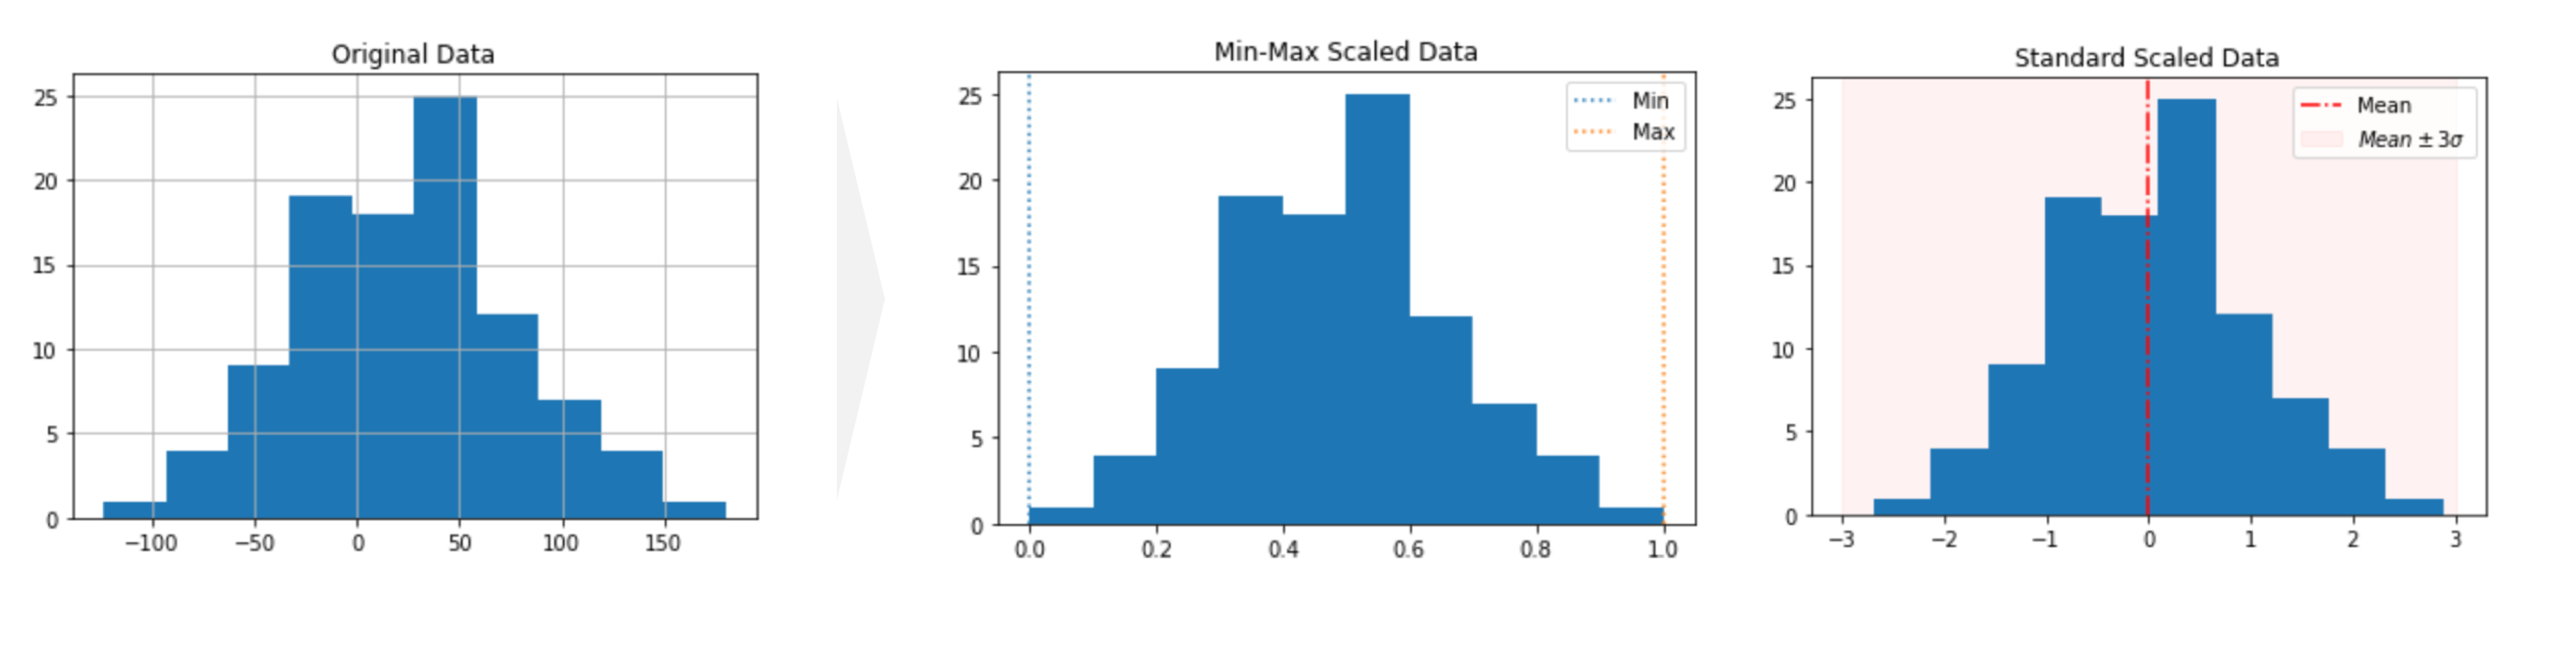
\includegraphics[width=\textwidth,height=\textheight,keepaspectratio]{Images/Theoretical basis/normalization.png}
    \caption{Chuẩn hóa dữ liệu}
\end{figure}

\subsubsection{Các phương pháp chuẩn hóa}

Hai phương pháp chuẩn hóa phổ biến là:

\begin{enumerate}
    \item \textbf{Min-Max Scaler:} Đưa dữ liệu về phạm vi [0, 1] bằng cách sử dụng công thức:

    $x_{norm} = \frac{x - x_{min}}{x_{max} - x_{min}}$

    trong đó: 
    \begin{itemize}
        \item $x$ là giá trị ban đầu
        \item $x_{norm}$ là giá trị sau khi chuẩn hóa 
        \item $x_{min}$ là giá trị nhỏ nhất của đặc trưng 
        \item $x_{max}$ là giá trị lớn nhất của đặc trưng 
    \end{itemize}
    \item \textbf{Standard Scaler:} Đưa dữ liệu về phân phối chuẩn có trung bình bằng 0 và độ lệch chuẩn bằng 1 bằng cách sử dụng công thức:

    $x_{norm} = \frac{x - \mu}{\sigma}$

    trong đó: 
    \begin{itemize}
        \item $x$ là giá trị ban đầu 
        \item $x_{norm}$ là giá trị sau khi chuẩn hóa 
        \item $\mu$ là trung bình của đặc trưng 
        \item $\sigma$ là độ lệch chuẩn của đặc trưng 
    \end{itemize}
\end{enumerate}

\subsubsection{Lợi ích}
\begin{itemize}
\item Cải thiện tốc độ huấn luyện.
\item Tăng độ chính xác của mô hình.
\item Giảm overfitting.
\item Ổn định quá trình huấn luyện.
\end{itemize}

\subsubsection{Hạn chế}
\begin{itemize}
\item Min-Max Scaler nhạy cảm với outliers.
\item Standard Scaler có thể không phù hợp với dữ liệu không tuân theo phân phối chuẩn.
\end{itemize}

\subsection{Giới thiệu về thư viện Tensorflow}
\indent TensorFlow chính là thư viện mã nguồn mở cho machine learning nổi tiếng nhất thế giới, được phát triển bởi các nhà nghiên cứu từ Google. Việc hỗ trợ mạnh mẽ các phép toán học để tính toán trong machine learning và deep learning đã giúp việc tiếp cận các bài toán trở nên đơn giản, nhanh chóng và tiện lợi hơn nhiều. 

\indent Các hàm được dựng sẵn trong thư viện cho từng bài toán cho phép TensorFlow xây dựng được nhiều neural network. Nó còn cho phép bạn tính toán song song trên nhiều máy tính khác nhau, thậm chí trên nhiều CPU, GPU trong cùng 1 máy hay tạo ra các dataflow graph - đồ thị luồng dữ liệu để dựng nên các model. Nếu bạn muốn chọn con đường sự nghiệp trong lĩnh vực A.I. này, nắm rõ những điều cơ bản của TensorFlow thực sự rất quan trọng.

\begin{figure}[H]
    \centering
    
\includegraphics[width=\textwidth,height=\textheight,keepaspectratio]{Images/Theoretical basis/TensorFlow_logo.png}
    \caption{Thư viện Tensorflow}
    \label{fig:enter-label}
\end{figure}

\subsubsection{Nguyên lý hoạt động}
\indent TensorFlow là một thư viện mã nguồn mở được thiết kế để thực hiện các phép tính số phức tạp thông qua cấu trúc đồ thị (graph). Cách hoạt động của TensorFlow dựa trên việc xây dựng và xử lý các mô hình học máy thông qua đồ thị tính toán, bao gồm các bước cơ bản sau:

\begin{itemize}
    \item \textbf{Xây dựng đồ thị tính toán:} Người dùng định nghĩa cấu trúc đồ thị, trong đó các nút (nodes) đại diện cho các phép tính toán (operations), và các cạnh (edges) biểu diễn luồng dữ liệu (dạng tensor) giữa các nút.
    \item \textbf{Định nghĩa hàm mất mát:} Hàm mất mát được sử dụng để đo lường sự khác biệt giữa đầu ra dự đoán của mô hình và giá trị thực tế. Đây là thước đo chính để tối ưu hóa mô hình.
    \item \textbf{Tối ưu hóa mô hình:} TensorFlow sử dụng các thuật toán tối ưu hóa như Gradient Descent để điều chỉnh các tham số trong mô hình, giảm giá trị của hàm mất mát.
    \item \textbf{Huấn luyện mô hình:} Dữ liệu huấn luyện được đưa vào mô hình, các tham số được cập nhật lặp đi lặp lại qua nhiều vòng huấn luyện để tối ưu hóa kết quả dự đoán.
    \item \textbf{Thực thi đồ thị qua Session:} Để thực hiện các phép tính, TensorFlow sử dụng Session, một môi trường chạy giúp thực thi đồ thị tính toán đã được xây dựng. Các session này cho phép TensorFlow phân phối các tác vụ tính toán trên nhiều thiết bị như CPU, GPU hoặc TPU.
    \item \textbf{Đánh giá mô hình:} Sau khi huấn luyện, mô hình được kiểm tra trên tập dữ liệu kiểm định để đánh giá hiệu suất và khả năng tổng quát.
    \item \textbf{Sử dụng mô hình:} Mô hình đã được huấn luyện có thể được sử dụng để dự đoán hoặc phân loại trên các dữ liệu mới, phù hợp với bài toán cụ thể.
\end{itemize}
\begin{figure}[H]
    \centering
    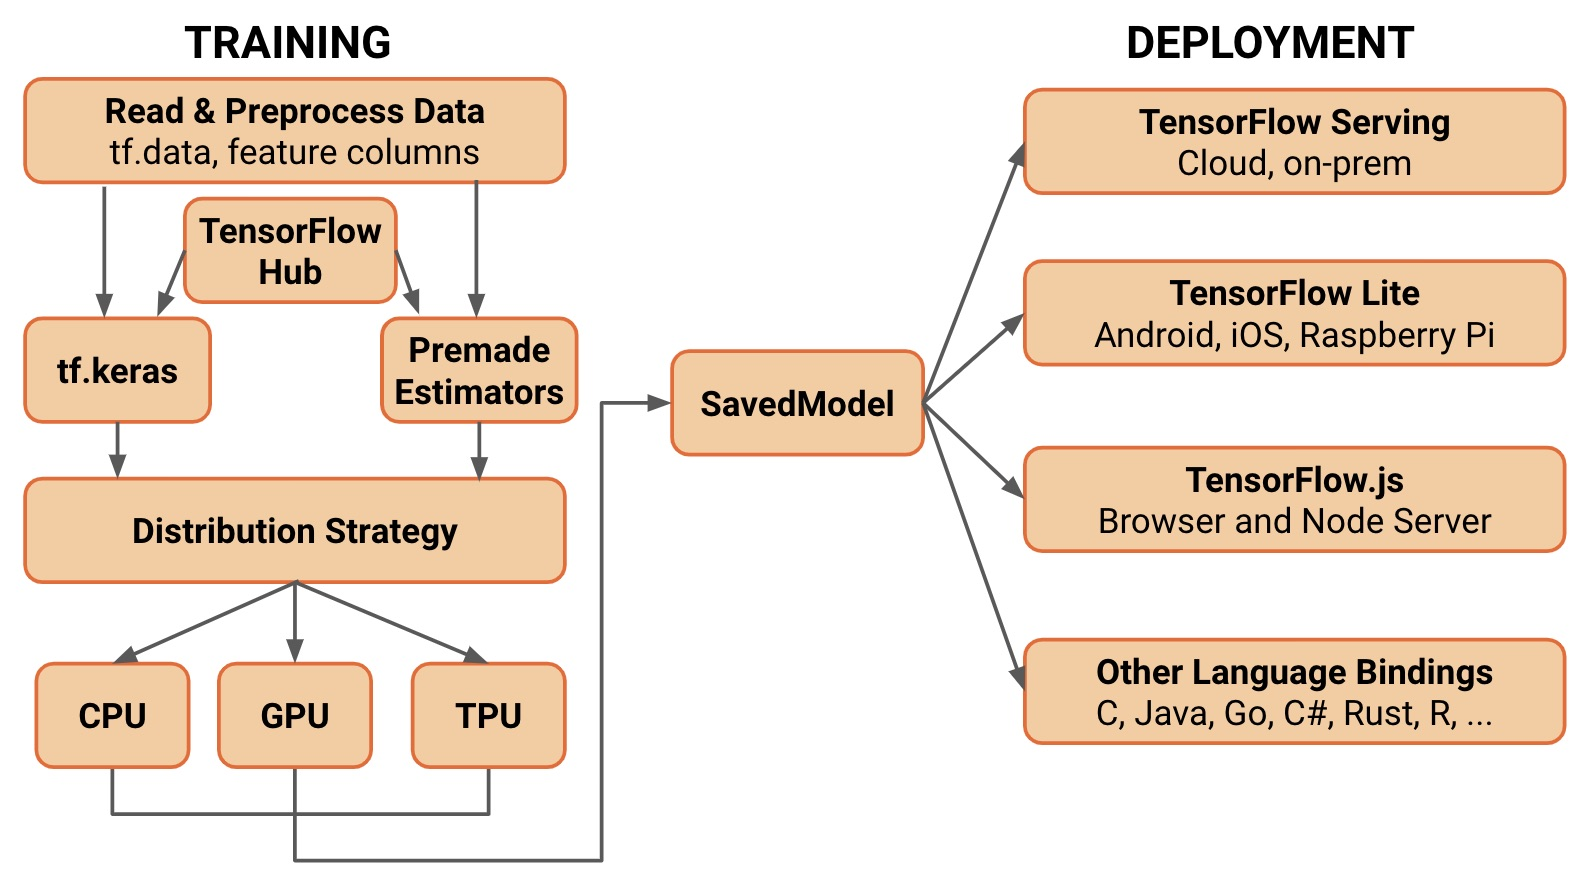
\includegraphics[width=\textwidth,height=\textheight,keepaspectratio]{Images/Theoretical basis/nguyen-li-hoat-dong-tensorflow.jpeg}
    \caption{Nguyên lý hoặc động của Tensorflow}
    \label{fig:enter-label}
\end{figure}


\subsubsection{Thuộc tính cơ bản trong Tensorflow}
\indent Về cơ bản thì các thuộc tính của TensorFlow bao gồm:
\begin{itemize}
    \item \textbf{Tensors:} 
    \begin{itemize}
        \item Tensor là cấu trúc dữ liệu trung tâm trong TensorFlow, đại diện cho các mảng đa chiều với kiểu dữ liệu đồng nhất.
        \item Tensor có thể mang giá trị là dữ liệu đầu vào, kết quả trung gian hoặc đầu ra của mô hình.
    \end{itemize}
    \begin{figure}[H]
        \centering
        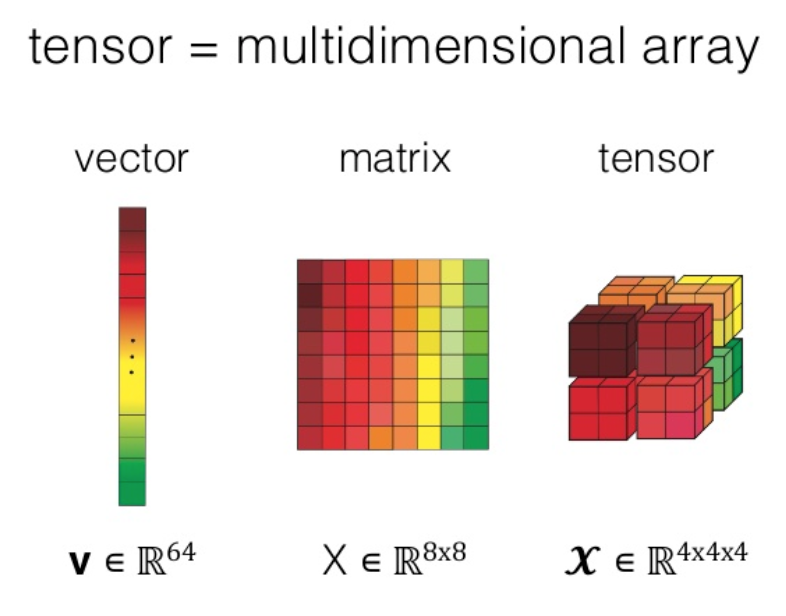
\includegraphics[width=\textwidth,height=\textheight,keepaspectratio]{Images/Theoretical basis/tensor.png}
        \caption{Hình ảnh minh họa của một tensor và so sánh với vector và ma trận.}
        \label{fig:enter-label}
    \end{figure}
    \item \textbf{Phép tính (Operations):} 
    \begin{itemize}
        \item TensorFlow thực hiện các phép tính trên tensors thông qua các operations (toán tử).
        \item Các phép tính cơ bản bao gồm cộng, trừ, nhân, chia và nhiều phép toán học nâng cao khác.
        \item Các operations này được biểu diễn dưới dạng các nút trong đồ thị tính toán.
    \end{itemize}
    \item \textbf{Biến(Variables):} 
    \begin{itemize}
        \item Biến được sử dụng để lưu trữ các giá trị có thể thay đổi trong quá trình huấn luyện mô hình, chẳng hạn như các tham số của mô hình.
        \item Giá trị của biến có thể được khởi tạo và cập nhật trong suốt quá trình huấn luyện.
    \end{itemize}

    \item \textbf{Đồ thị(Graphs):}
    \begin{itemize}
        \item Đồ thị là một biểu đồ tính toán biểu diễn mối quan hệ giữa các phép tính và dữ liệu.
        \item TensorFlow sử dụng đồ thị để tối ưu hóa việc tính toán và triển khai mô hình trên nhiều thiết bị khác nhau, bao gồm CPU, GPU và TPU.
    \end{itemize}
    \item \textbf{Sessions:}
    \begin{itemize}
        \item Session là một phiên làm việc trong TensorFlow, nơi các phép tính trong đồ thị được thực thi.
        \item Session quản lý các biến, phép tính và thực hiện quá trình huấn luyện hoặc dự đoán.
    \end{itemize}
    \begin{figure}[H]
        \centering
        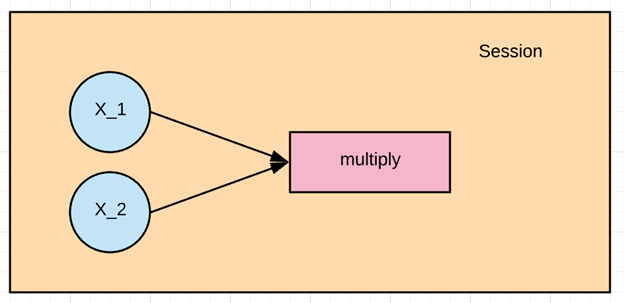
\includegraphics[width=\textwidth,height=\textheight,keepaspectratio]{Images/Theoretical basis/083018_0508_WhatisTenso2.png}
        \caption{Minh họa cho 1 graph, session, operation và variable.}
        \label{fig:enter-label}
    \end{figure}
    \item \textbf{Placeholders:} 
    \begin{itemize}
        \item Placeholders là các "nơi trống" trong đồ thị, được sử dụng để nhận dữ liệu đầu vào tại thời điểm chạy.
        \item Điều này cho phép mô hình linh hoạt khi xử lý nhiều loại dữ liệu khác nhau trong quá trình huấn luyện hoặc kiểm tra.
    \end{itemize}
\end{itemize}

Các thuộc tính trên tạo thành nền tảng mạnh mẽ, giúp TensorFlow trở thành công cụ hàng đầu trong việc xây dựng, huấn luyện và triển khai các mô hình học máy hiện đại.

\subsubsection{Ưu điểm của TensorFlow}

\begin{itemize}
    \item \textbf{Tính linh hoạt cao:} 
    \begin{itemize}
        \item TensorFlow hỗ trợ nhiều loại mô hình học máy, từ học có giám sát đến học không giám sát và học tăng cường.
        \item Người dùng có thể dễ dàng tùy chỉnh mô hình để phù hợp với các bài toán cụ thể, từ mạng nơ-ron đơn giản đến các kiến trúc phức tạp như CNN, RNN, hay Transformer.
    \end{itemize}
    \item \textbf{Khả năng mở rộng mạnh mẽ:} 
    \begin{itemize}
        \item TensorFlow được thiết kế để chạy trên nhiều nền tảng khác nhau, bao gồm máy tính cá nhân, máy chủ, GPU, TPU và thậm chí là các thiết bị di động.
        \item Điều này giúp người dùng triển khai mô hình trên các môi trường khác nhau mà không cần thay đổi mã nguồn.
    \end{itemize}
    \item \textbf{Hiệu suất cao:} 
    \begin{itemize}
        \item TensorFlow tận dụng sức mạnh của phần cứng, hỗ trợ tính toán song song và tối ưu hóa hiệu suất thông qua GPU và TPU.
        \item Công cụ này cũng cung cấp các thuật toán tối ưu hóa hiệu quả, giúp giảm thời gian huấn luyện mô hình.
    \end{itemize}
    \item \textbf{Cộng đồng hỗ trợ lớn:}
    \begin{itemize}
        \item TensorFlow có một cộng đồng người dùng toàn cầu lớn mạnh, cung cấp nhiều tài liệu học tập, hướng dẫn và giải pháp cho các vấn đề kỹ thuật.
        \item Với nguồn tài liệu phong phú, người dùng dễ dàng tìm kiếm hỗ trợ từ cộng đồng hoặc các diễn đàn trực tuyến.
    \end{itemize}
    \item \textbf{Hỗ trợ triển khai mô hình:}
    \begin{itemize}
        \item TensorFlow cho phép triển khai mô hình trên nhiều nền tảng, từ máy tính cá nhân đến các ứng dụng di động, web và đám mây.
        \item TensorFlow Lite giúp tối ưu hóa mô hình cho các thiết bị có hiệu năng hạn chế như điện thoại thông minh và thiết bị IoT.
    \end{itemize}
    \item \textbf{Thư viện phong phú:} 
    \begin{itemize}
        \item TensorFlow cung cấp nhiều thư viện mở rộng như TensorFlow.js (dành cho trình duyệt web), TensorFlow Lite (dành cho thiết bị di động) và TensorFlow Extended (hỗ trợ quy trình phát triển mô hình từ đầu đến cuối).
        \item Người dùng có thể dễ dàng tích hợp các thư viện này vào dự án của mình.
    \end{itemize}
\end{itemize}

\subsection{Giới thiệu về Arduino LilyPad}
\indent Arduino LilyPad là một phiên bản đặc biệt của bo mạch Arduino, được thiết kế dành riêng cho các ứng dụng điện tử gắn vào vải (e-textiles) và thiết bị điện tử có thể đeo (wearables). Bo mạch này có cấu trúc phẳng, nhẹ và có thể được may trực tiếp vào trang phục hoặc phụ kiện bằng chỉ dẫn điện.

\indent Arduino LilyPad được phát triển bởi Leah Buechley và SparkFun Electronics, dựa trên vi điều khiển ATmega168 hoặc ATmega328V. Đây là một giải pháp lý tưởng cho các dự án điện tử sáng tạo, nơi tính thẩm mỹ và tính linh hoạt trong thiết kế được ưu tiên.
\begin{figure}[H]
    \centering
    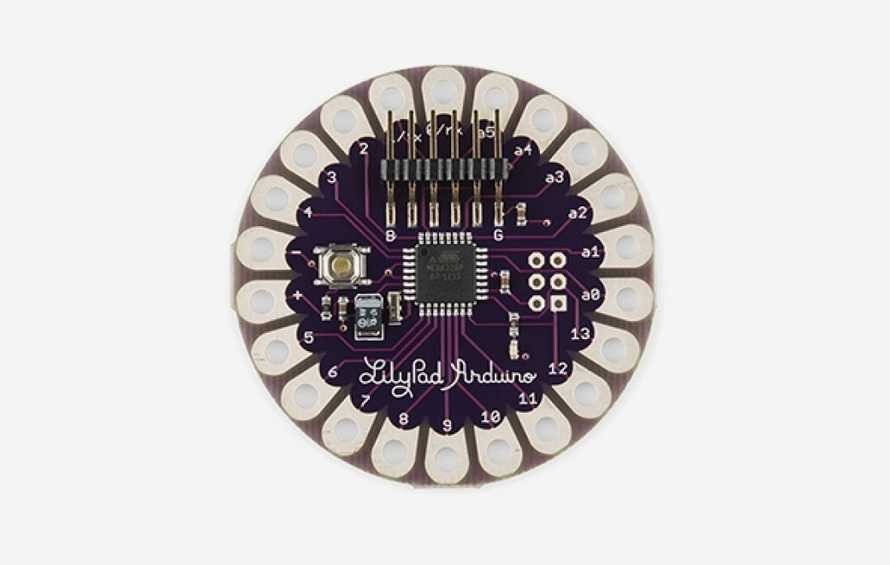
\includegraphics[width=\textwidth,height=\textheight,keepaspectratio]{Images/Theoretical basis/lilypad_main.jpg}
    \caption{Board mạch Arduino Lilypad}
    \label{fig:enter-label}
\end{figure}

\begin{longtblr}[
  caption = {Thông số kỹ thuật của Arduino Lilypad},
]{
  width = \linewidth,
  colspec = {Q[404]Q[521]},
  hlines,
  vlines,
}
Vi điều khiển          & ATmega168 hoặc ATmega328V \\
Điện áp hoạt động      & 2.7-5.5 V                                                                                 \\
Điện áp đầu vào        & 2.7-5.5 V                                                                                 \\
Số chân I/O            & 14                                                                                        \\
Số kênh PWM            & 6                                                                                         \\
Số kênh đầu vào Analog & 6                                                                                         \\
Dòng điện mỗi chân     & 40mA                                                                                      \\
Bộ nhớ Flash           & 16 KB                                                                                     \\
SRAM                   & 1 KB                                                                                      \\
EEPROM                 & 512 bytes                                                                                 \\
Tần số xung            & 8 MHz                                                                                     
\end{longtblr}



\indent Ứng dụng tiêu biểu của Arduino Lilypad:
\begin{itemize}
    \item \textbf{Trang phục thông minh:} Arduino LilyPad có thể được sử dụng để theo dõi thông số cơ thể, điều khiển ánh sáng hoặc tích hợp cảm biến vào trang phục.
    \item \textbf{Thiết bị đeo tay:} Nó có thể làm nền tảng cho các sản phẩm như găng tay thông minh, vòng tay theo dõi sức khỏe hoặc thiết bị điều khiển bằng cử chỉ.
    \item \textbf{Dự án nghệ thuật:} LilyPad được sử dụng rộng rãi trong các dự án nghệ thuật sáng tạo, kết hợp công nghệ với thiết kế thẩm mỹ.
\end{itemize}
Với thiết kế nhỏ gọn và khả năng tích hợp cao, Arduino LilyPad là lựa chọn lý tưởng cho các nhà sáng tạo muốn kết hợp công nghệ với thời trang và các thiết bị cá nhân hóa.



\subsection{Giới thiệu về Flex sensor}


\subsubsection{Tổng quan} 

\indent Flex Sensor (Cảm biến uốn cong) là một loại cảm biến đặc biệt hoạt động dựa trên nguyên tắc thay đổi điện trở khi bị uốn cong. Loại cảm biến này thường được sử dụng để đo lường và theo dõi mức độ uốn cong hoặc góc độ của một bề mặt hoặc cấu trúc.

\indent Flex Sensor có thiết kế nhỏ gọn, linh hoạt và thường được sản xuất với hai kích thước phổ biến:
\begin{itemize}
    \item 2.2 inch (khoảng 5.588 cm)
    \item 4.5 inch (khoảng 11.43 cm)
\end{itemize}

\indent Nhờ khả năng thay đổi giá trị điện trở tỷ lệ thuận với mức độ uốn cong, cảm biến này trở thành một giải pháp hiệu quả cho nhiều ứng dụng, đặc biệt trong các dự án liên quan đến thiết bị đeo, robot hoặc hệ thống điều khiển bằng cử chỉ.

\indent Cảm biến uốn cong thường được sử dụng kết hợp với các mạch điện để chuyển đổi thay đổi điện trở thành tín hiệu điện áp, từ đó dễ dàng xử lý bằng các bộ vi điều khiển hoặc các hệ thống khác.

\indent Với độ nhạy cao và tính linh hoạt, cảm biến uốn cong là một lựa chọn lý tưởng trong các dự án cần theo dõi chuyển động hoặc đo lường độ biến dạng của bề mặt.

\begin{figure}[H]
    \centering
    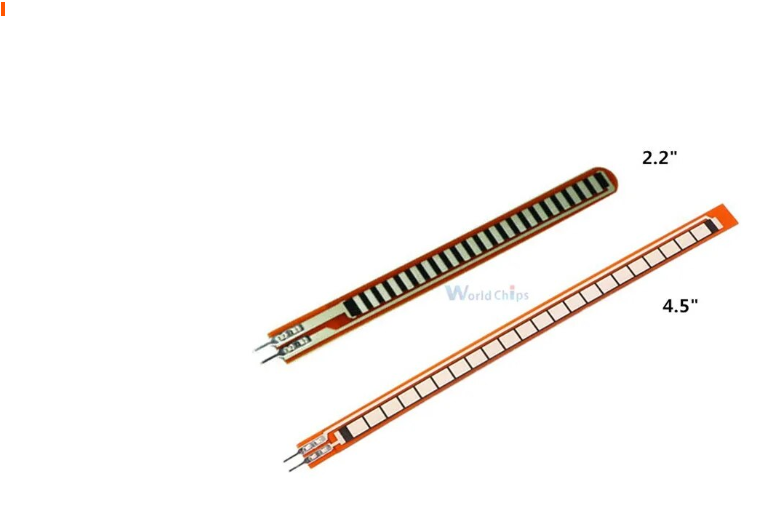
\includegraphics[width=9cm]{Images/Theoretical basis/flex sensor.png}
\caption{Flex sensor}
\end{figure}

\subsubsection{Nguyên lý hoạt động}

\indent Cảm biến uốn cong hoạt động dựa trên sự thay đổi điện trở của một lớp mực dẫn đặc biệt được phủ trên bề mặt cảm biến. Khi cảm biến bị uốn cong, các đặc tính của lớp mực dẫn thay đổi, dẫn đến sự biến đổi giá trị điện trở. Cơ chế hoạt động của cảm biến bao gồm các đặc điểm chính sau:

\begin{enumerate}[-]
    \item \textbf{Trạng thái thẳng:} Khi cảm biến ở trạng thái thẳng, lớp mực dẫn không bị biến dạng, và giá trị điện trở thường dao động ở mức thấp, khoảng 25k$\Omega$.
    \item \textbf{Trạng thái uốn cong:} Khi cảm biến bị uốn, lớp mực dẫn bị kéo căng, làm giảm diện tích tiếp xúc và tăng trở kháng của nó. Ở góc uốn cong 90°, giá trị điện trở có thể tăng lên đến 100k$\Omega$ hoặc hơn, tùy thuộc vào thiết kế và loại cảm biến.
    \item \textbf{Trạng thái phục hồi:} Khi cảm biến được duỗi thẳng lại, lớp mực dẫn trở về trạng thái ban đầu, và giá trị điện trở cũng quay về mức trước đó.
\end{enumerate}

\begin{figure}[H]
    \centering
    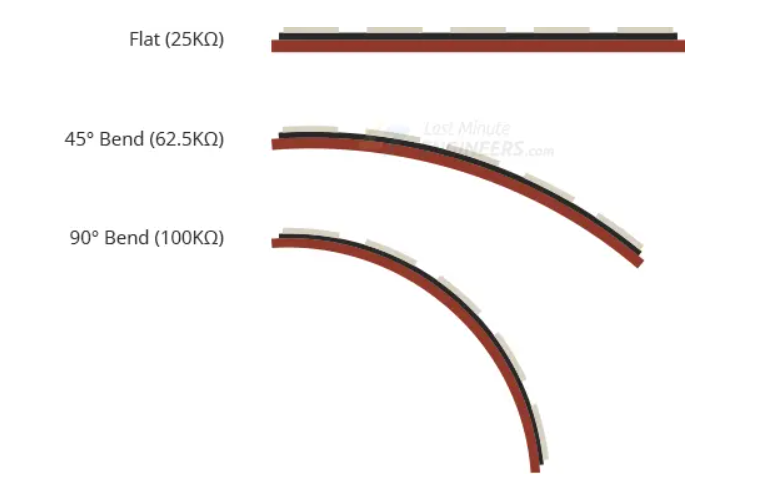
\includegraphics[width=11cm]{Images/Theoretical basis/flex sensor 1.png}
\caption{Hình dạng uốn cong của flex sensor}
\end{figure}

\subsubsection{Đọc giá trị}

\indent Việc đọc giá trị từ cảm biến uốn cong được thực hiện thông qua một mạch điện đơn giản, thường là mạch chia điện áp. Cảm biến uốn cong được kết hợp với một điện trở cố định để tạo ra một tín hiệu điện áp thay đổi, tương ứng với mức độ uốn cong của cảm biến. Điện áp này sau đó được đo và xử lý bởi bộ vi điều khiển hoặc mạch xử lý tín hiệu.

\begin{figure}[H]
    \centering
    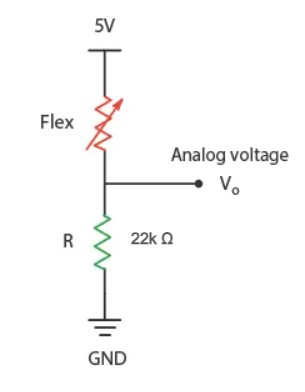
\includegraphics[width=5cm]{Images/Theoretical basis/flex sensor 2.jpg}
\caption{Sơ đồ nối dây của flex sensor}
\end{figure}

\indent Lưu ý rằng điện áp đầu ra mà bạn đo là mức giảm điện áp qua trở kháng kéo xuống, không phải là giảm điện áp qua cảm biến uốn cong (Flex Sensor).

\indent Chúng ta có thể sử dụng công thức sau để tính toán điện áp đầu ra (Vo).
\[ V_0 = \frac{V_{cc} \cdot R}{R + R_{\text{flex}}} \]

\indent Trong trường hợp này, điện áp đầu ra giảm khi bán kính uốn cong tăng lên.
\subsection{Giới thiệu về cảm biến con quay gia tốc}
\subsubsection{Tổng quan}
\indent Cảm biến con quay gia tốc là một thiết bị được sử dụng để đo lường sự gia tốc của một vật thể theo các trục không gian. Thiết bị này hoạt động dựa trên nguyên lý của lực quán tính, thường kết hợp với công nghệ MEMS (Micro-Electro-Mechanical Systems) để đạt được độ chính xác cao trong kích thước nhỏ gọn.

\indent Bên trong cảm biến, một khối lượng nhỏ được treo bằng các lò xo siêu nhỏ. Khi cảm biến chịu tác động của gia tốc, khối lượng này di chuyển do lực quán tính, và sự chuyển động này được chuyển đổi thành tín hiệu điện thông qua các cơ chế đo lường như:
\begin{enumerate}[-]
    \item \textbf{Hiệu ứng điện dung:} Sử dụng sự thay đổi điện dung giữa các phần tử trong cảm biến để đo mức độ di chuyển.
    \item \textbf{Hiệu ứng áp điện (Piezoelectric):} Sử dụng các vật liệu tạo điện áp khi chịu lực cơ học để đo sự dịch chuyển.
\end{enumerate}
\indent Cảm biến gia tốc thường được thiết kế để đo gia tốc theo ba trục: X, Y và Z. Điều này giúp xác định chính xác chuyển động, tư thế hoặc vị trí của vật thể trong không gian.

\subsubsection{Nguyên lý hoạt động}
\subsubsubsection{Hiệu ứng điện dung:}
\indent Cấu trúc lò xo - khối nặng - giảm xóc: Cấu trúc này chuyển đổi gia tốc của khung cảm biến thành sự dịch chuyển của khối nặng chứng minh, và phương pháp cảm biến điện dung được áp dụng để chuyển đổi sự dịch chuyển này thành tín hiệu điện tử tỷ lệ với gia tốc được áp dụng.
\begin{figure}[H]
    \centering
    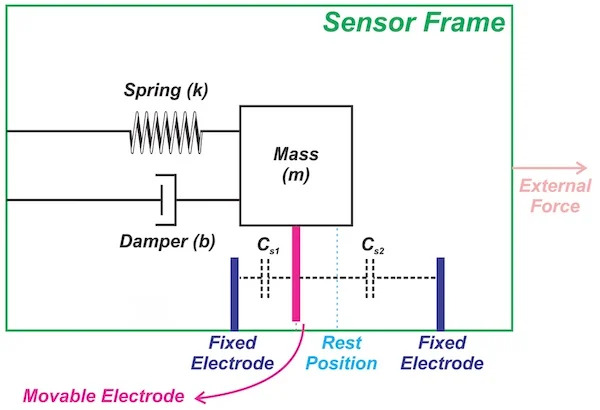
\includegraphics[width=\textwidth,height=\textheight,keepaspectratio]{Images/Theoretical basis/168_Introduction_to_Capacitive_Acceleration_Sensors_Figure_3.jpeg}
    \caption{Cấu trúc của một cảm biến gia tốc sử dụng phương pháp điện dung}
    \label{fig:capacitive_sensor}
\end{figure}
\indent Phương pháp cảm biến điện dung: Có hai bản điện cực được gắn cố định vào khung cảm biến cùng với một điện cực di động được kết nối với khối lượng tham chiếu. Thiết kế này hình thành hai tụ điện biến thiên C1 và C2, như được hiển thị trong hình \ref{fig:capacitive_sensor}.

\indent Khi khối lượng tham chiếu di chuyển theo một hướng dưới ảnh hưởng của gia tốc, điện dung giữa điện cực di động và một trong hai điện cực cố định tăng lên trong khi điện dung của tụ điện kia giảm xuống. Bằng cách đo đạc sự thay đổi điện dung của hai tụ điện trên, và kết hợp với khối lượng tham chiếu có sẳn ta có thể tính toán được gia tốc đầu vào.

\subsubsubsection{Hiệu ứng áp điện (Piezoelectric):}
\indent Hiệu ứng Piezoelectric là hiện tượng mà một số vật liệu nhất định có khả năng tạo ra điện tích khi chịu áp lực cơ học. Từ “Piezoelectric” bắt nguồn từ từ tiếng Hy Lạp “piezein”, có nghĩa là “ấn hoặc nén”, mô tả chính xác quá trình tạo ra điện năng thông qua áp lực.

\indent Hiệu ứng này xảy ra ở mức độ vi mô, khi áp dụng một lực cơ học dẫn đến sự di chuyển của các điện tích dương và âm trong cấu trúc tinh thể của vật liệu. Sự dịch chuyển này tạo ra một cực điện và hình thành một điên áp đi qua vật liệu.

\indent Hiệu ứng Piezoelectric là một quá trình có thể đảo ngược: vật liệu thể hiện hiệu ứng piezoelectric cũng sẽ bị biến dạng cơ học nếu đặt một điện áp đi qua nó.

Ví dụ, các tinh thể titanate zirconate chì sẽ tạo ra dòng điện Piezoelectric khi cấu trúc tĩnh của chúng bị biến dạng khoảng 0,1\% so với kích thước gốc. Ngược lại, những tinh thể giống như vậy sẽ thay đổi khoảng 0,1\% kích thước tĩnh của chúng khi áp dụng một điện trường bên ngoài.

\indent Hiệu ứng Piezoelectric đã được khai thác trong nhiều ứng dụng hữu ích, bao gồm sản xuất và phát hiện âm thanh, in phun piezoelectric, tạo ra điện năng điện áp cao, như một bộ tạo xung trong các thiết bị điện tử, trong microbalances, để điều khiển một đầu phun siêu âm, và trong việc tập trung siêu mịn của các bộ phận quang học.
\begin{figure}[H]
    \centering
    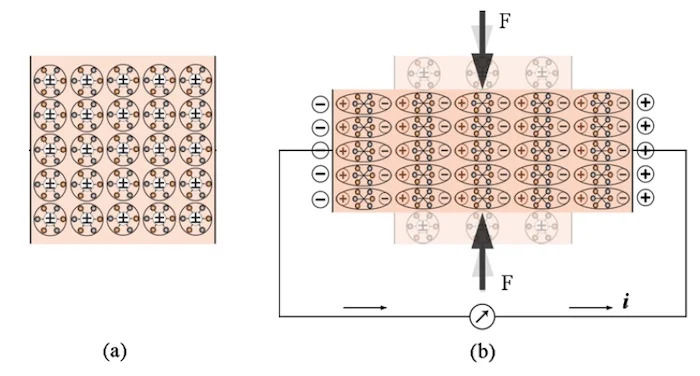
\includegraphics[width=\textwidth,height=\textheight,keepaspectratio]{Images/Theoretical basis/intro_piezo_accelerometers_figure_1.jpeg}
    \caption{Hiệu ứng Piezoelectric}
    \label{fig:pio_prin}
\end{figure}
\indent Cấu trúc của cảm biến gia tốc bao gồm một phần tử piezoelectric để kết nối một lượng khối lượng cố định với thân cảm biến. Khi khung cảm biến tăng tốc do lực bên ngoài, khối lượng tham chiếu có xu hướng giữ nguyên vị trí do quán tính và làm biến dạng nhẹ phần tử piezoelectric.
\indent Nếu nối hai điện cực với nhau thông qua một sợi dây như mô tả trong \ref{fig:pio_prin}, thì các electron tự do trong dây dẫn sẽ chảy về phía điện cực tích điện dương và tạo ra một dòng điện. Dòng điện này tích tụ các electron tự do trên điện cực dương và tạo ra một điện trường ngược hướng với trường ban đầu được tạo ra bởi hiệu ứng Piezoelectric.

\indent Hiệu ứng này giải thích tại sao dòng điện do lực tĩnh tạo ra chỉ có thể tồn tại trong một khoảng thời gian ngắn. Dòng điện tiếp tục cho đến khi điện trường do sự tích tụ của các electron tự do triệt tiêu trường khỏi hiệu ứng Piezoelectric.
\begin{figure}[H]
    \centering
    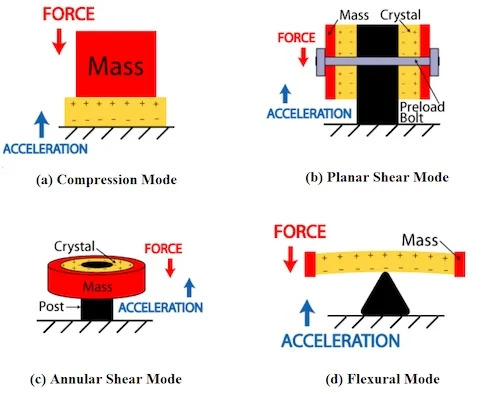
\includegraphics[width=\textwidth,height=\textheight,keepaspectratio]{Images/Theoretical basis/intro_piezo_accelerometers_figure_2.jpeg}
    \caption{Các kiểu thiết kế cơ học của cảm biến gia tốc}
    \label{fig:piozDesin}
\end{figure}
\indent Các kiểu thiết kế cơ học phổ biến của cảm biến gia tốc sử dụng hiệu ứng Piezoelectric:
\begin{itemize}
    \item \textbf{Thiết kế theo chế độ nén:} THiết kế này rất đơn giản, chỉ bao gồm một bản thiết bị có hiệu ứng Piezoelectric và một khối lượng tham chiếu. Khi xảy ra gia tốc, lực quán tính sẽ làm cho khối lượng tham chiếu ép chặt vào tấm vật liệu áp điện từ đó tạo ra dòng điện.
    \item \textbf{Thiết theo chế độ trượt:} Gồm hai loại là trượt trên một tấm phẳng hoặc thiết kế trượt trên một khối hình nhẫn. Về cơ bản thì hai kiểu thiết kế này có cùng ngueyen lý hoạt động. Tinh thể được kẹp giữa trụ trung tâm và khối lượng thâm chiếu bên ngoài. Khối lượng càng nhiều thì lực trượt tác dụng lên tinh thể càng lớn đối với một gia tốc nhất định. Cấu trúc này giúp gia tốc kế cứng chắc, tạo ra dải tần số cao và do tinh thể không tiếp xúc trực tiếp với  cảm biến nên các hiệu ứng biến dạng và chuyển tiếp nhiệt được giảm thiểu.
    \item \textbf{Thiết kế theo chế độ uốn:} thiết kế này sử dụng các tấm tinh thể có hình chữ nhật hoặc hình đĩa. Sự uốn cong của tinh thể có thể xảy ra do khối lượng của chính tinh thể đối lập với gia tốc hoặc để tăng cường sự uốn cong, trọng lượng bổ sung có thể được kẹp hoặc liên kết với tinh thể. Gia tốc kế ở chế độ uốn ít cứng hơn khi so sánh với thiết kế nén hoặc trượt, cung cấp cho chúng dải tần số giới hạn. Ngoài ra, do tinh thể phải chịu mức độ căng áp lực cao nên chúng dễ bị hỏng hơn các loại khác nếu bị sốc hoặc rung quá mức.
\end{itemize}

\subsubsection{Giới thiệu về module cảm biến ITG 3200}
\begin{figure}[H]
    \centering
    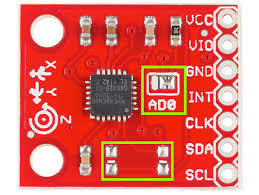
\includegraphics[width=0.5\textwidth,height=\textheight,keepaspectratio]{Images/Theoretical basis/ITG3200.jpg}
    \caption{Cảm biến gia tốc góc ITG 3200}
    \label{fig:capacitive_sensor}
\end{figure}
\indent Module cảm biến ITG 3200 là một loại cảm biến con quay gia tốc 3 trục, sử dụng công nghệ MEMS để đo góc quay và vận tốc góc. Cảm biến này có khả năng cung cấp dữ liệu về các chuyển động xoay trên ba trục không gian X, Y và Z. ITG 3200 có độ chính xác cao và tốc độ đáp ứng nhanh, phù hợp với nhiều ứng dụng yêu cầu đo đạc chuyển động như điều khiển robot, máy bay không người lái (drone), hệ thống ổn định, và các thiết bị đo lường khác.
\\
\textbf{Các đặc điểm chính của ITG 3200:}
\begin{itemize}
\item \textbf{Cảm biến 3 trục:} Đo lường góc quay và vận tốc góc trên ba trục không gian.
\item \textbf{Độ phân giải cao:} Cảm biến có thể cung cấp các giá trị đo chính xác với độ phân giải lên đến 14-bit.
 \item \textbf{Tốc độ lấy mẫu:} Cảm biến hỗ trợ tốc độ lấy mẫu lên đến 8 kHz, giúp thu thập dữ liệu nhanh và chính xác.
 \item \textbf{Giao tiếp I2C:} ITG 3200 sử dụng giao tiếp I2C để truyền tải dữ liệu, giúp dễ dàng kết nối với các vi điều khiển và hệ thống nhúng.
\item \textbf{Nguồn cấp}: Được cấp nguồn từ 2.3V đến 3.4V, giúp tiết kiệm năng lượng trong các ứng dụng di động hoặc thiết bị nhúng.
\item \textbf{Bộ lọc tích hợp} Cảm biến này có tích hợp bộ lọc kỹ thuật số để giảm nhiễu và cải thiện độ chính xác của dữ liệu.
\end{itemize}
\indent \textbf{Ứng dụng của ITG 3200:}
\begin{itemize}
\item \textbf{Điều khiển ổn định:} ITG 3200 được sử dụng trong các hệ thống ổn định để đo chuyển động quay, giúp duy trì sự cân bằng của các thiết bị như drone và robot.
\item \textbf{Thiết bị đo lường:} Sử dụng trong các thiết bị đo đạc góc quay chính xác, chẳng hạn như thiết bị đeo thông minh và các hệ thống tự động.
 \item \textbf{Các hệ thống điều khiển:} Được sử dụng trong các hệ thống điều khiển tự động, giúp phát hiện và xử lý chuyển động quay trong thời gian thực.
\end{itemize}

\subsection{Giới thiệu về module bluetooth HC05}
\begin{figure}[H]
    \centering
    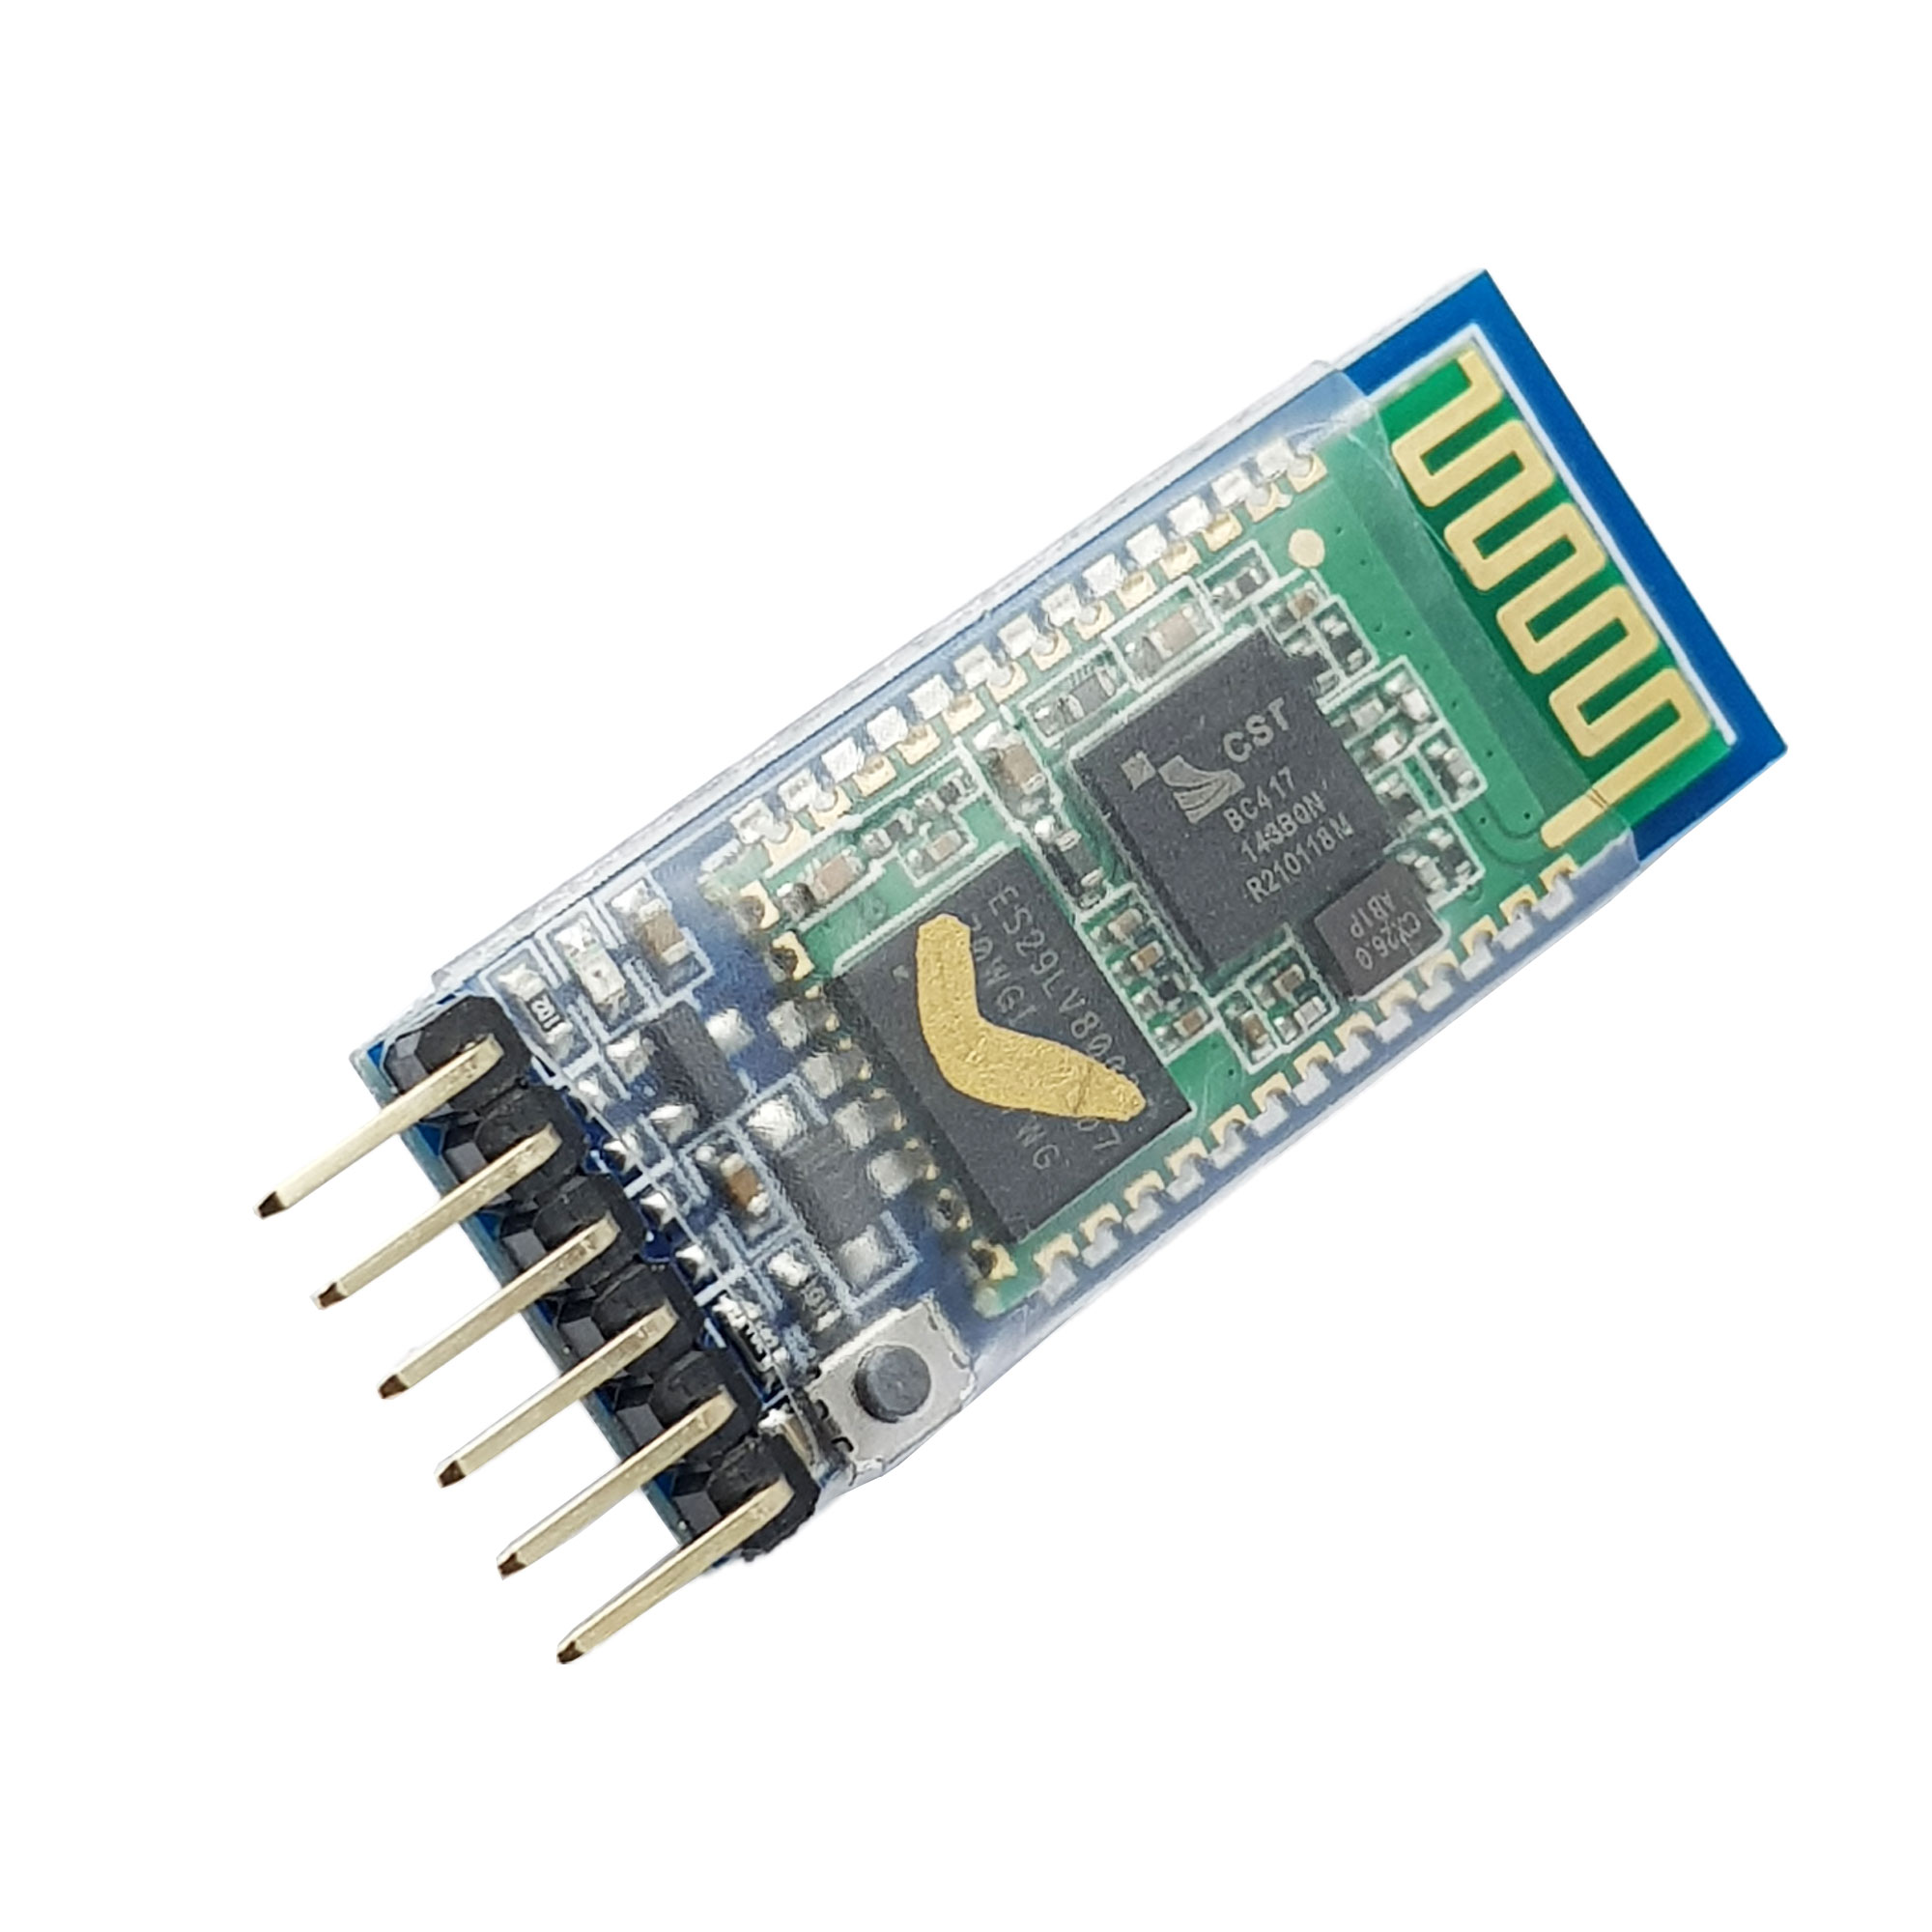
\includegraphics[width=0.5\textwidth,height=\textheight,keepaspectratio]{Images/Theoretical basis/hc05.jpg}
    \caption{module bluetooth HC-05}
    \label{fig:capacitive_sensor}
\end{figure}

\indent Module Bluetooth HC-05 là một mô-đun giao tiếp không dây sử dụng chuẩn Bluetooth 2.0, cho phép kết nối các thiết bị điện tử với nhau qua giao thức Bluetooth. Đây là một module phổ biến và dễ sử dụng trong các dự án điện tử và IoT (Internet of Things), giúp các thiết bị như vi điều khiển, cảm biến hoặc các thiết bị di động kết nối với nhau một cách thuận tiện.
\\
\textbf{Các đặc điểm chính của HC-05:}
\begin{itemize}
\item \textbf{Chế độ hoạt động:} HC-05 hỗ trợ hai chế độ hoạt động: Master (chủ) và Slave (phụ). Chế độ Master cho phép HC-05 kết nối với các thiết bị khác, trong khi chế độ Slave cho phép module kết nối với một thiết bị khác như điện thoại hoặc máy tính.
\item \textbf{Giao tiếp Serial (UART):} HC-05 sử dụng giao tiếp UART (Universal Asynchronous Receiver/Transmitter) để trao đổi dữ liệu với các vi điều khiển và các thiết bị điện tử khác, giúp dễ dàng tích hợp vào các mạch điện tử.
 \item \textbf{Khoảng cách truyền tín hiệu:} HC-05 có thể truyền tín hiệu Bluetooth trong phạm vi lên tới 10 mét, tùy thuộc vào môi trường và các yếu tố xung quanh.
\item \textbf{Nguồn cấp}: Module hoạt động với nguồn cung cấp từ 3.3V đến 5V, tương thích với các hệ thống sử dụng vi điều khiển phổ biến như Arduino.
\item \textbf{Tốc độ truyền dữ liệu:} HC-05 có tốc độ truyền dữ liệu lên đến 3 Mbps, cho phép truyền tải thông tin nhanh chóng và hiệu quả giữa các thiết bị.
\end{itemize}
\textbf{Ứng dụng của HC-05:}
\begin{itemize}
\item \textbf{Kết nối không dây:} HC-05 có thể được sử dụng trong các dự án yêu cầu kết nối không dây giữa các thiết bị như Arduino với điện thoại thông minh, máy tính hoặc các thiết bị khác hỗ trợ Bluetooth.
\item \textbf{Điều khiển từ xa:} Module này được ứng dụng trong các hệ thống điều khiển từ xa, giúp người dùng điều khiển thiết bị điện tử thông qua ứng dụng di động hoặc máy tính.
 \item \textbf{Hệ thống IoT:} HC-05 là một lựa chọn phổ biến trong các hệ thống IoT, nơi các thiết bị cần giao tiếp với nhau qua mạng Bluetooth để truyền dữ liệu hoặc điều khiển từ xa.
\end{itemize}
\subsection{Giới thiệu về ngôn ngữ ký hiệu}
\indent Ngôn ngữ ký hiệu là phương tiện giao tiếp chính thức của cộng đồng người khiếm thính, được sử dụng để biểu đạt ý tưởng và cảm xúc thông qua các cử chỉ tay và động tác cơ thể. Mỗi ngôn ngữ ký hiệu có cấu trúc ngữ pháp và từ vựng riêng, khác biệt với ngôn ngữ nói và thường được sử dụng bởi những người không thể nghe hoặc không thể nói.

\indent Ngôn ngữ ký hiệu không chỉ bao gồm các động tác tay mà còn sử dụng biểu cảm khuôn mặt, cử chỉ của các bộ phận cơ thể như mắt, đầu và cơ thể để truyền đạt thông điệp. Điều này giúp ngôn ngữ ký hiệu trở thành một hệ thống giao tiếp toàn diện, có thể biểu đạt đầy đủ các ý tưởng phức tạp như trong ngôn ngữ nói.

\indent Ngôn ngữ ký hiệu ở Việt Nam đã được hình thành từ rất lâu. Nhưng do trước đây chưa có nhà khoa học nào tìm hiểu,nghiên cứu về nó nên người Việt Nam không nghĩ và đã không xem những dấu hiệu mà người điếc sử dụng là ngôn ngữ. Họ cho rằng đó chỉ là những điệu bộ khua tay của người điếc để cố gắng giao tiếp do thiếu ngôn ngữ. Mãi đến năm 1996, một tiến sĩ ngôn ngữ học người Mỹ James C. Woodward, người đã từng làm việc với William Stokoe tại trường đại học Gallaudet của Mỹ, đã sang Việt Nam thực hiện nghiên cứu về ngôn ngữ ký hiệu của cộng đồng người điếc ở Việt Nam. Theo nghiên cứu của ông, ở Việt Nam hiện có ít nhất 3 ngôn ngữ ký hiệu phổ biến (được cộng đồng người điếc sử dụng nhiều nhất). Ông đã dùng tên của những địa danh này để đặt tên cho 3 ngôn ngữ ký hiệu đó: Ngôn ngữ ký hiệu Hà Nội, ngôn ngữ ký hiệu Hải Phòng, và ngôn ngữ ký hiệu Thành phố Hồ Chí Minh.

\indent Sau đó, đã có thêm những dự án ở Việt Nam:dự án Giáo dục hòa nhập cho trẻ điếc 1998-2001 (Viện Khoa học Giáo dục- tổ chức Pearl S. Buck, Int), dư án Giáo dục trung học và đại học cho người Điếc Việt Nam 2000 cho đến hiện tại (Sở GD-ĐT Đồng Nai và GS TS JAMES C. WOODWARD) để thực hiện việc thu thập lại những dấu hiệu của người điếc Việt Nam và tìm hiểu về ngữ pháp của ngôn ngữ này. Công việc này đã kích thích thêm nhiều nhà khoa học ở Việt Nam cũng bắt đầu tìm hiểu về ngữ pháp của ngôn ngữ ký hiệu Việt Nam.

\indent Để một người có thể diễn đạt được ngôn ngữ ký hiệu đòi hỏi một hoặc nhiều yếu tố dưới đây:
\begin{itemize}
    \item \textbf{Vị trí làm kí hiệu:} Vị trí làm kí hiệu là vị trí của bàn tay so với cơ thể khi làm kí hiệu. Vị trí làm kí hiệu khác nhau thể hiện những ý nghĩa khác nhau. Khoảng không gian để thể hiện kí hiệu được giới hạn từ đỉnh đầu, khoảng không gian phía trước cơ thể mở rộng đến độ rộng của hai khuỷu tay ở hai phía, lưng và hông.
    \item  \textbf{Hình dạng bàn tay:} Hình dạng bàn tay là các hình dạng khác nhau của bàn tay khi thực hiện kí hiệu.
    \item \textbf{Sự chuyển động của tay:} Sự chuyển động của tay là những cử động của tay khi làm kí hiệu, bao gồm chuyển động đơn (một chuyển động trong một lần làm kí hiệu), và chuyển động kép (nhiều chuyển động trong một lần làm kí hiệu). Nhìn vào mũi tên trong hình vẽ của kí hiệu chúng ta biết được sự chuyển động của tay.
    \item \textbf{Chiều hướng của tay:} Chiều hướng của tay khi làm kí hiệu bao gồm chiều hướng của lòng bàn tay và chiều hướng của các ngón tay.
    \item \textbf{Sự diễn tả không bằng tay:} Sự diễn tả không bằng tay là những cử chỉ, điệu bộ, nét mặt, cử động của cơ thể kèm theo.
\end{itemize}
\begin{figure}[H]
    \centering
    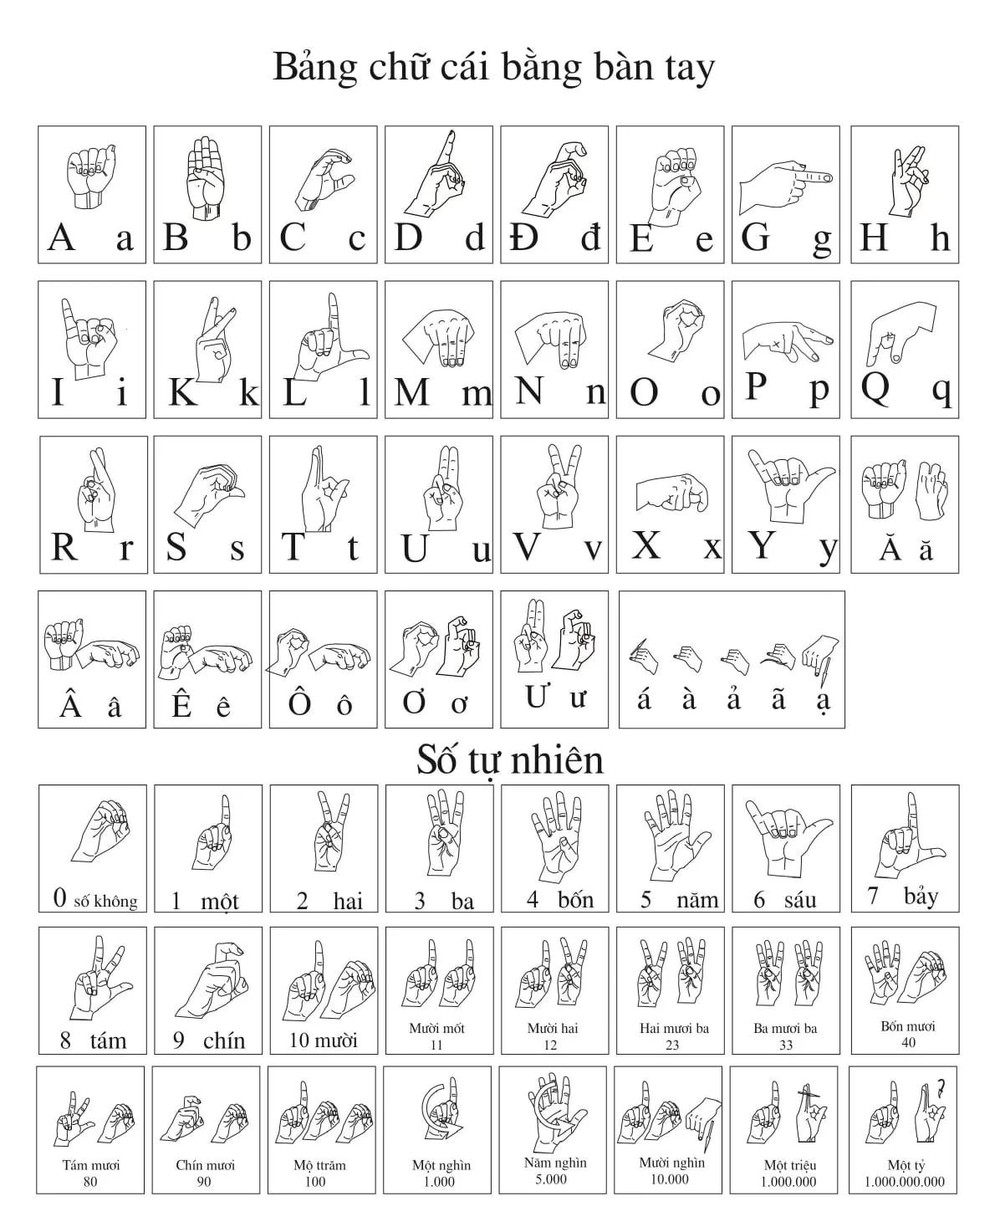
\includegraphics[width=\textwidth,height=\textheight,keepaspectratio]{Images/Theoretical basis/bangsochu.jpg}
    \caption{Bảng ngôn ngữ kí hiệu}
    \label{fig:enter-label}
\end{figure}



\newpage
%%%%%%%%%%%%%%%%%%%%%%%%%%%%%%%%%
\section{Kiến trúc hệ thống}
Hệ thống được thiết kế với hai module với chức năng của từng module được mô tả dưới đây:
\begin{itemize}
    \item \textbf{Module thu thập dữ liệu cử chỉ:} Đầu vào của khối này là dữ liệu cử chỉ được thu thạp từ các cảm biến uốn cong và cảm biến gia tốc. Dẽ liệu sau khi thu thập sẽ được đóng goi và gửi về module nhận dạng cử chỉ.
    \item \textbf{Module nhận dạng cử chỉ} Dữ liệu được gửi về từ module thu thập sẽ được xử lý, phân loại và đình hình lại dữ liệu để đưa vào mô hình LSTM. Đầu ra của mô hình LSTM sẽ là kết quả dự đoán cử chỉ dưới dạng văn bản và sẽ được chuyển đổi thành giọng nói qua khối Text-to-speech.
    \item \textbf{Module chuyển văn bản thành giọng nói}: Khi nhận được output đầu ra, module này có chức năng chuyển đầu ra từ dạng one-hot-code output sang dạng văn bản, từ văn bản đó sử dụng thư viện pyttsx3 để phát ra âm thanh như mong muốn đã được cấu hình trước đó trong file config
\end{itemize}
\begin{figure}[H]
    \centering
    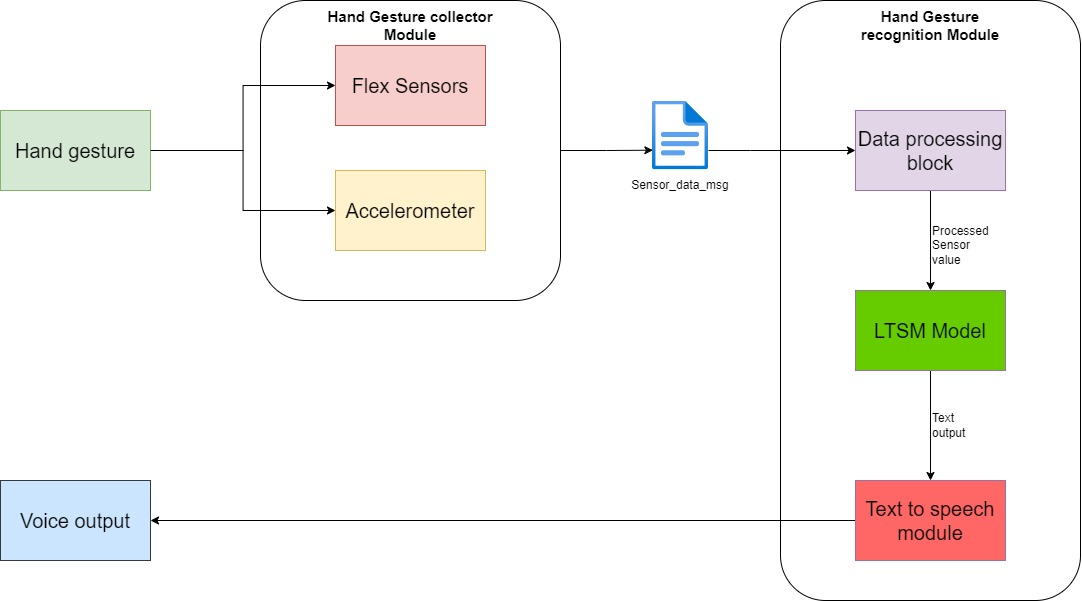
\includegraphics[width=\textwidth,height=\textheight,keepaspectratio]{Images/Theoretical basis/FlexArchitecture.jpg}
    \caption{Kiến trúc tổng quan của hệ thống}
    \label{fig:enter-label}
\end{figure}
\textbf{Mô tả luồng dữ liệu }
\textbf{Hand Gesture} (Cử chỉ tay): Cử chỉ tay là đầu vào của hệ thống. Các cảm biến uốn cong và gia tốc kế trong mô-đun thu thập cử chỉ tay sẽ ghi nhận và gửi dữ liệu này đến khối xử lý dữ liệu.\

\textbf{Sensor Data Message }(Thông điệp dữ liệu cảm biến): Dữ liệu từ cảm biến được đóng gói thành thông điệp và truyền tới mô-đun nhận diện cử chỉ tay.\

\textbf{Processed Sensor Value} (Giá trị cảm biến đã xử lý): Dữ liệu cảm biến được xử lý trong khối xử lý dữ liệu và các đặc trưng được trích xuất.\

\textbf{Text Output} (Đầu ra văn bản): Mô hình LSTM dự đoán cử chỉ tay và chuyển đổi nó thành văn bản.\

\textbf{Voice Output} (Đầu ra giọng nói): Văn bản từ mô hình LSTM được chuyển đổi thành giọng nói và phát ra ngoài thông qua mô-đun chuyển văn bản thành giọng nói.\


Hệ thống này bao gồm hai mô-đun chính và một module phụ: một mô-đun thu thập cử chỉ tay, một mô-đun nhận diện cử chỉ tay và module phát âm thanh. Mô-đun thu thập cử chỉ tay sử dụng các cảm biến uốn cong và gia tốc kế để ghi nhận dữ liệu cử chỉ tay, sau đó truyền dữ liệu này đến mô-đun nhận diện cử chỉ tay. Tại đây, dữ liệu cảm biến được xử lý và đưa vào mô hình LSTM để dự đoán cử chỉ tay dưới dạng văn bản. Cuối cùng, văn bản này được chuyển đổi thành giọng nói dựa trên module phát âm thanh


\subsection{Module thu thập dữ liệu cử chỉ}
\begin{figure}[H]
    \centering
    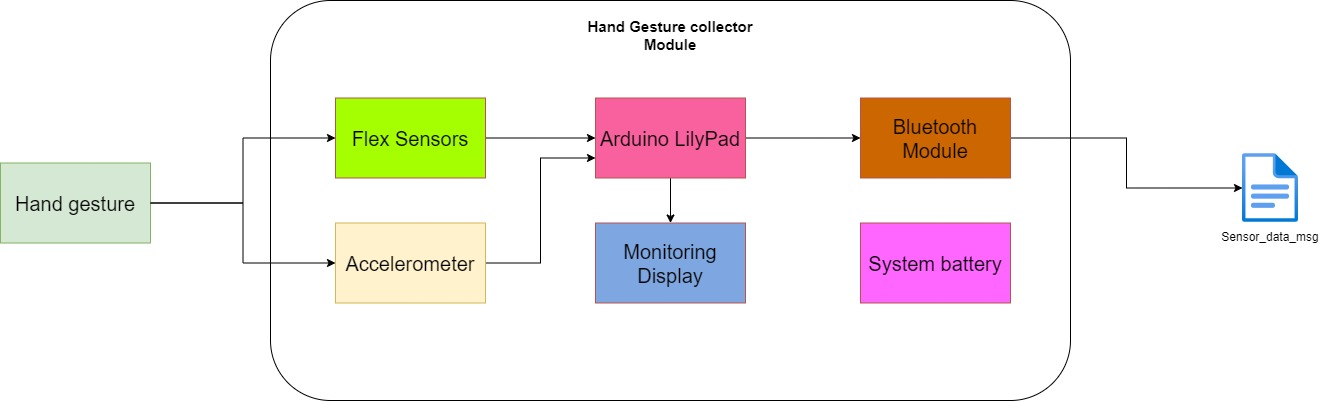
\includegraphics[width=\textwidth,height=\textheight,keepaspectratio]{Images/Theoretical basis/HandGestureCollector.jpg}
    \caption{Kiến trúc module thu thập dữ liệu cử chỉ}
    \label{fig:enter-label}
\end{figure}

Sơ đồ mô tả một hệ thống thu thập cử chỉ tay, gồm các thành phần sau:
\begin{itemize}
\item 1. Hand gesture (Cử chỉ tay): Đây là đầu vào của hệ thống, là các cử chỉ tay cần được nhận diện.
\item 2. Flex Sensors (Cảm biến uốn cong): Nhận tín hiệu từ cử chỉ tay và chuyển tiếp đến Arduino LilyPad.
\item 3. Accelerometer (Gia tốc kế): Cũng nhận tín hiệu từ cử chỉ tay và chuyển tiếp đến Arduino LilyPad.
\item 4. Arduino LilyPad: Xử lý dữ liệu nhận được từ Flex Sensors và Accelerometer. Sau đó, chuyển tiếp dữ liệu này đến các thành phần khác.
\item 5. Monitoring Display (Màn hình giám sát): Hiển thị dữ liệu và thông tin từ Arduino LilyPad để người dùng có thể theo dõi.
\item 6. Bluetooth Module (Mô-đun Bluetooth): Truyền dữ liệu từ Arduino LilyPad tới file data
\item 7. System Battery (Pin hệ thống): Cung cấp năng lượng cho toàn bộ hệ thống.
\end{itemize}


Dữ liệu được thu thập từ cử chỉ tay sẽ được xử lý và truyền đi qua mô-đun Bluetooth, sau đó lưu vào file data
\subsection{Module nhận dạng cử chỉ}
\begin{figure}[H]
    \centering
    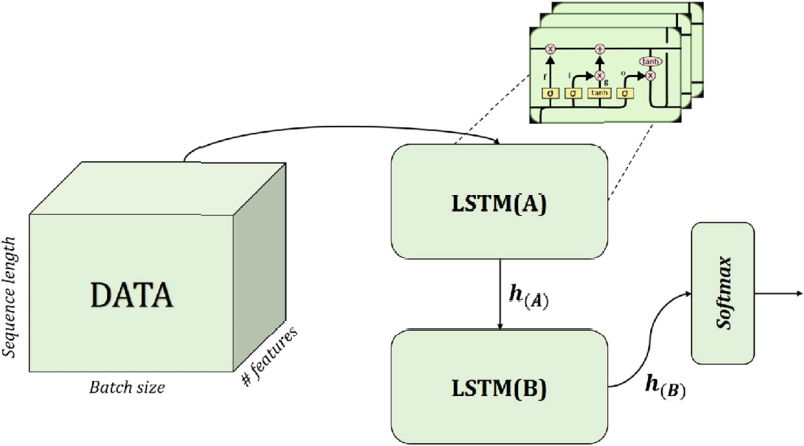
\includegraphics[width=\textwidth,height=\textheight,keepaspectratio]{Images/Theoretical basis/lstm model.png}
    \caption{Kiến trúc model dự đoán cử chỉ}
    \label{fig:enter-label}
\end{figure}

Sơ đồ mô tả một mô hình học sâu sử dụng LSTM (Long Short-Term Memory) để dự đoán xác suất của các hành động, như mua hoặc bán. Dưới đây là mô tả chi tiết của từng thành phần trong mô hình:
\begin{itemize}
     

\item 1. DATA (Dữ liệu):\\
   - Đầu vào của mô hình là một khối dữ liệu ba chiều với các thông số:\\
     - Sequence length: Độ dài chuỗi thời gian của dữ liệu.\\
     - Batch size: Kích thước lô, số lượng chuỗi thời gian trong một lô.\\
     - Features: Số lượng đặc trưng trong mỗi bước thời gian của chuỗi.

\item 2. LSTM(A):\\
   - Dữ liệu đầu vào được đưa vào lớp LSTM đầu tiên, gọi là LSTM(A). LSTM là một loại mạng nơ-ron hồi tiếp được thiết kế để xử lý và dự đoán các chuỗi dữ liệu thời gian.

\item 3. h(A):\\
   - Đầu ra của LSTM(A) là một vector ẩn (hidden vector), ký hiệu là h(A). Vector này lưu trữ thông tin trạng thái ẩn của LSTM sau khi xử lý dữ liệu đầu vào.

\item 4. LSTM(B):\\
   - Vector ẩn h(A) sau đó được đưa vào một lớp LSTM thứ hai, gọi là LSTM(B). Lớp này tiếp tục xử lý dữ liệu và tạo ra một vector ẩn mới, ký hiệu là h(B).

\item 5. h(B):\\
   - Đầu ra của LSTM(B) là vector ẩn h(B), lưu trữ thông tin trạng thái ẩn sau khi dữ liệu được xử lý qua hai lớp LSTM.

\item 6. Softmax:\\
   - Vector ẩn h(B) được đưa vào một lớp Softmax. Lớp này chuyển đổi vector thành các xác suất để dự đoán các hành động cụ thể.

\item 7. Output:\\
   - Đầu ra cuối cùng của mô hình là các xác suất được tạo ra bởi lớp Softmax, ví dụ như label 0,1,2 được mã hóa dưới dạng one-hot-code

\end{itemize}
Mô hình này có thể được sử dụng cho các ứng dụng như dự đoán thị trường chứng khoán hoặc các bài toán khác liên quan đến chuỗi thời gian, nơi việc xác định các hành động dựa trên dữ liệu lịch sử là quan trọng. Sơ đồ này minh họa cách dữ liệu được xử lý qua các lớp LSTM và sau đó chuyển đổi thành các xác suất đầu ra thông qua lớp Softmax.


\subsection{Module phát âm thanh}
\begin{figure}[H]
    \centering
    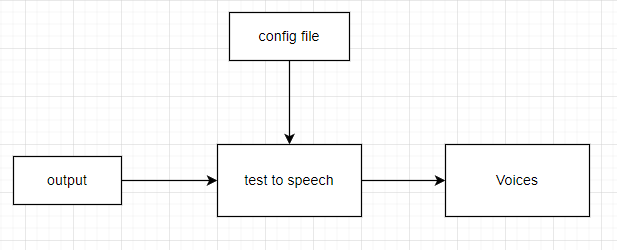
\includegraphics[width=\textwidth,height=\textheight,keepaspectratio]{Images/Theoretical basis/test2speech.png}
    \caption{Kiến trúc module chuyển đầu ra dự đoán thành giọng nói}
    \label{fig:enter-label}
\end{figure}

Sơ đồ mô tả module phát âm thanh sau khi dự đoán đúng một hành động sử dụng thư viện text-to-speech pyttsx3

Thư viện pyttsx3 cung cấp một giao diện đơn giản và nhất quán cho việc chuyển đổi văn bản thành giọng nói trên nhiều nền tảng. Kiến trúc của nó được thiết kế để trừu tượng hóa các chi tiết đặc thù của nền tảng, cho phép các nhà phát triển tập trung vào chức năng TTS ở mức cao. Các thành phần cốt lõi bao gồm bộ máy, trình điều khiển và cơ chế cấu hình, hoạt động cùng nhau để cung cấp tổng hợp giọng nói liền mạch và tùy chỉnh. Thiết kế của thư viện đảm bảo tính tương thích, linh hoạt và dễ sử dụng, biến nó thành công cụ mạnh mẽ để thêm khả năng TTS vào các ứng dụng Python.

Cụ thể âm thanh được phát ra khi có một output chỉ index trong file config giọng nói trước đó có sẵn, kiến trúc này sẽ lấy chính xác vị trí âm thanh giọng nói phát ra như mong muốn.
\newpage
%%%%%%%%%%%%%%%%%%%%%%%%%%%%%%%%%
\section{Hiện thực hệ thống}
\subsection{Hiện thực phần cứng}
\begin{figure}[H]
    \centering
    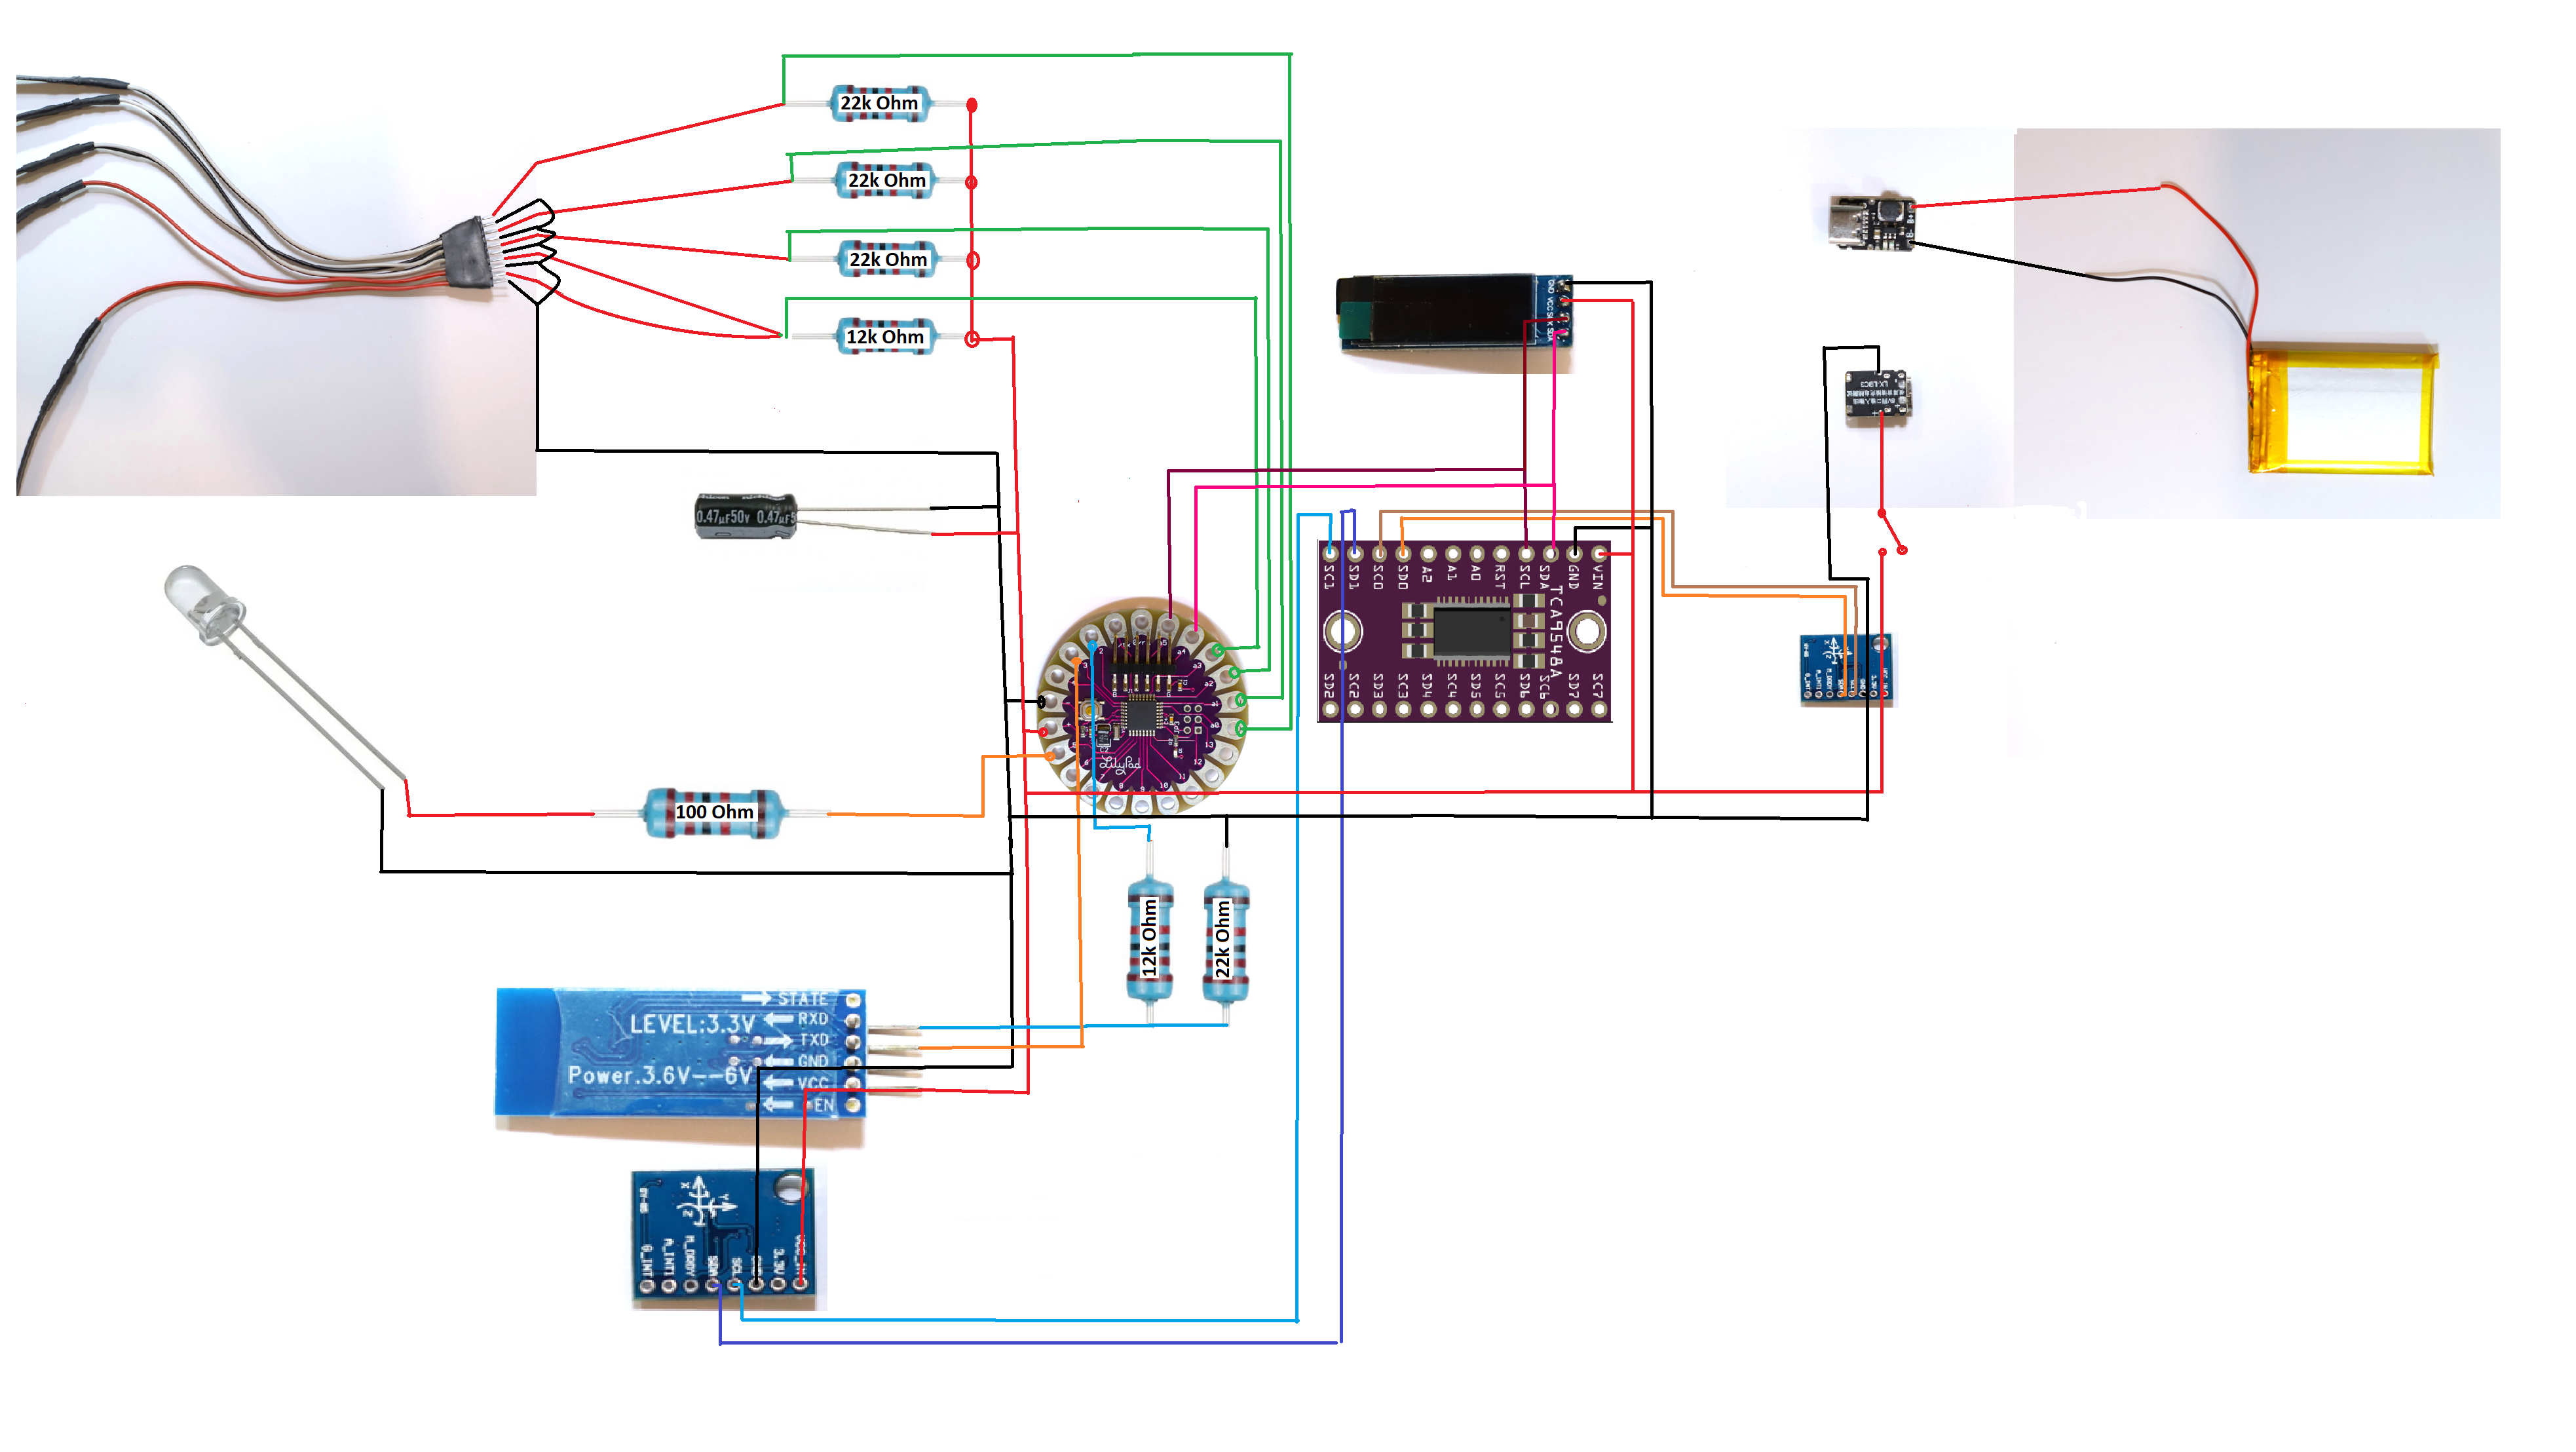
\includegraphics[width=\textwidth,height=\textheight,keepaspectratio]{Images/SystemImpl/schematic.png}
    \caption{Sơ đồ kết nối mạch}
    \label{fig:enter-label}
\end{figure}
Sơ đồ này mô tả kết nối của một mạch điện tử bao gồm nhiều thành phần như cảm biến, Arduino, màn hình hiển thị, mô-đun Bluetooth, và nguồn pin. Dưới đây là mô tả chi tiết các thành phần và kết nối của chúng:
\begin{itemize}
    \item Cảm biến Flex:\\
   - Cảm biến này có nhiều dây kết nối với các điện trở (22k Ohm và 12k Ohm).\\
   - Các dây này sau đó được kết nối với vi điều khiển (Arduino LilyPad).
   \item LED và Điện trở (100 Ohm):\\
   - LED được kết nối với một điện trở 100 Ohm và sau đó nối với vi điều khiển.
   \item Arduino LilyPad:\\
   - Đây là vi điều khiển trung tâm trong mạch, chịu trách nhiệm thu thập và xử lý dữ liệu từ các cảm biến.\\
   - Nó được kết nối với các cảm biến Flex, màn hình hiển thị, mô-đun Bluetooth và các điện trở khác.
  \item Màn hình hiển thị:\\
   - Màn hình hiển thị nhỏ (có thể là OLED) được kết nối với Arduino để hiển thị dữ liệu hoặc thông tin cần thiết.
  \item Mô-đun Bluetooth:\\
   - Mô-đun Bluetooth được kết nối để truyền dữ liệu không dây. Nó được cấp nguồn từ Arduino và được kết nối với các chân TX, RX của vi điều khiển.
  \item  Nguồn pin:\\
   - Một pin Lithium-Polymer (LiPo) được sử dụng để cung cấp năng lượng cho toàn bộ mạch.
  \item Các điện trở khác:\\
   - Có các điện trở khác trong mạch để điều chỉnh dòng điện và điện áp đi qua các thành phần.
  \item Mạch sạc và quản lý pin:\\
   - Một mạch quản lý pin (TP4056) được kết nối với pin để đảm bảo việc sạc an toàn và hiệu quả.
\end{itemize}

Dưới đây là mô tả kết nối chi tiết:

- Các dây từ cảm biến Flex được kết nối với các chân trên Arduino LilyPad thông qua các điện trở 22k Ohm và 12k Ohm.
- LED được kết nối với một điện trở 100 Ohm trước khi nối với Arduino LilyPad.
- Màn hình hiển thị được kết nối với các chân của Arduino LilyPad để hiển thị dữ liệu.
- Mô-đun Bluetooth được kết nối với các chân TX, RX, VCC, và GND của Arduino LilyPad.
- Pin LiPo cung cấp năng lượng qua mạch sạc TP4056, từ đó kết nối với Arduino và các thành phần khác để cấp nguồn.

Sơ đồ này minh họa rõ ràng cách các thành phần điện tử được kết nối với nhau để tạo thành một hệ thống hoàn chỉnh.
\begin{figure}[H]
    \centering
    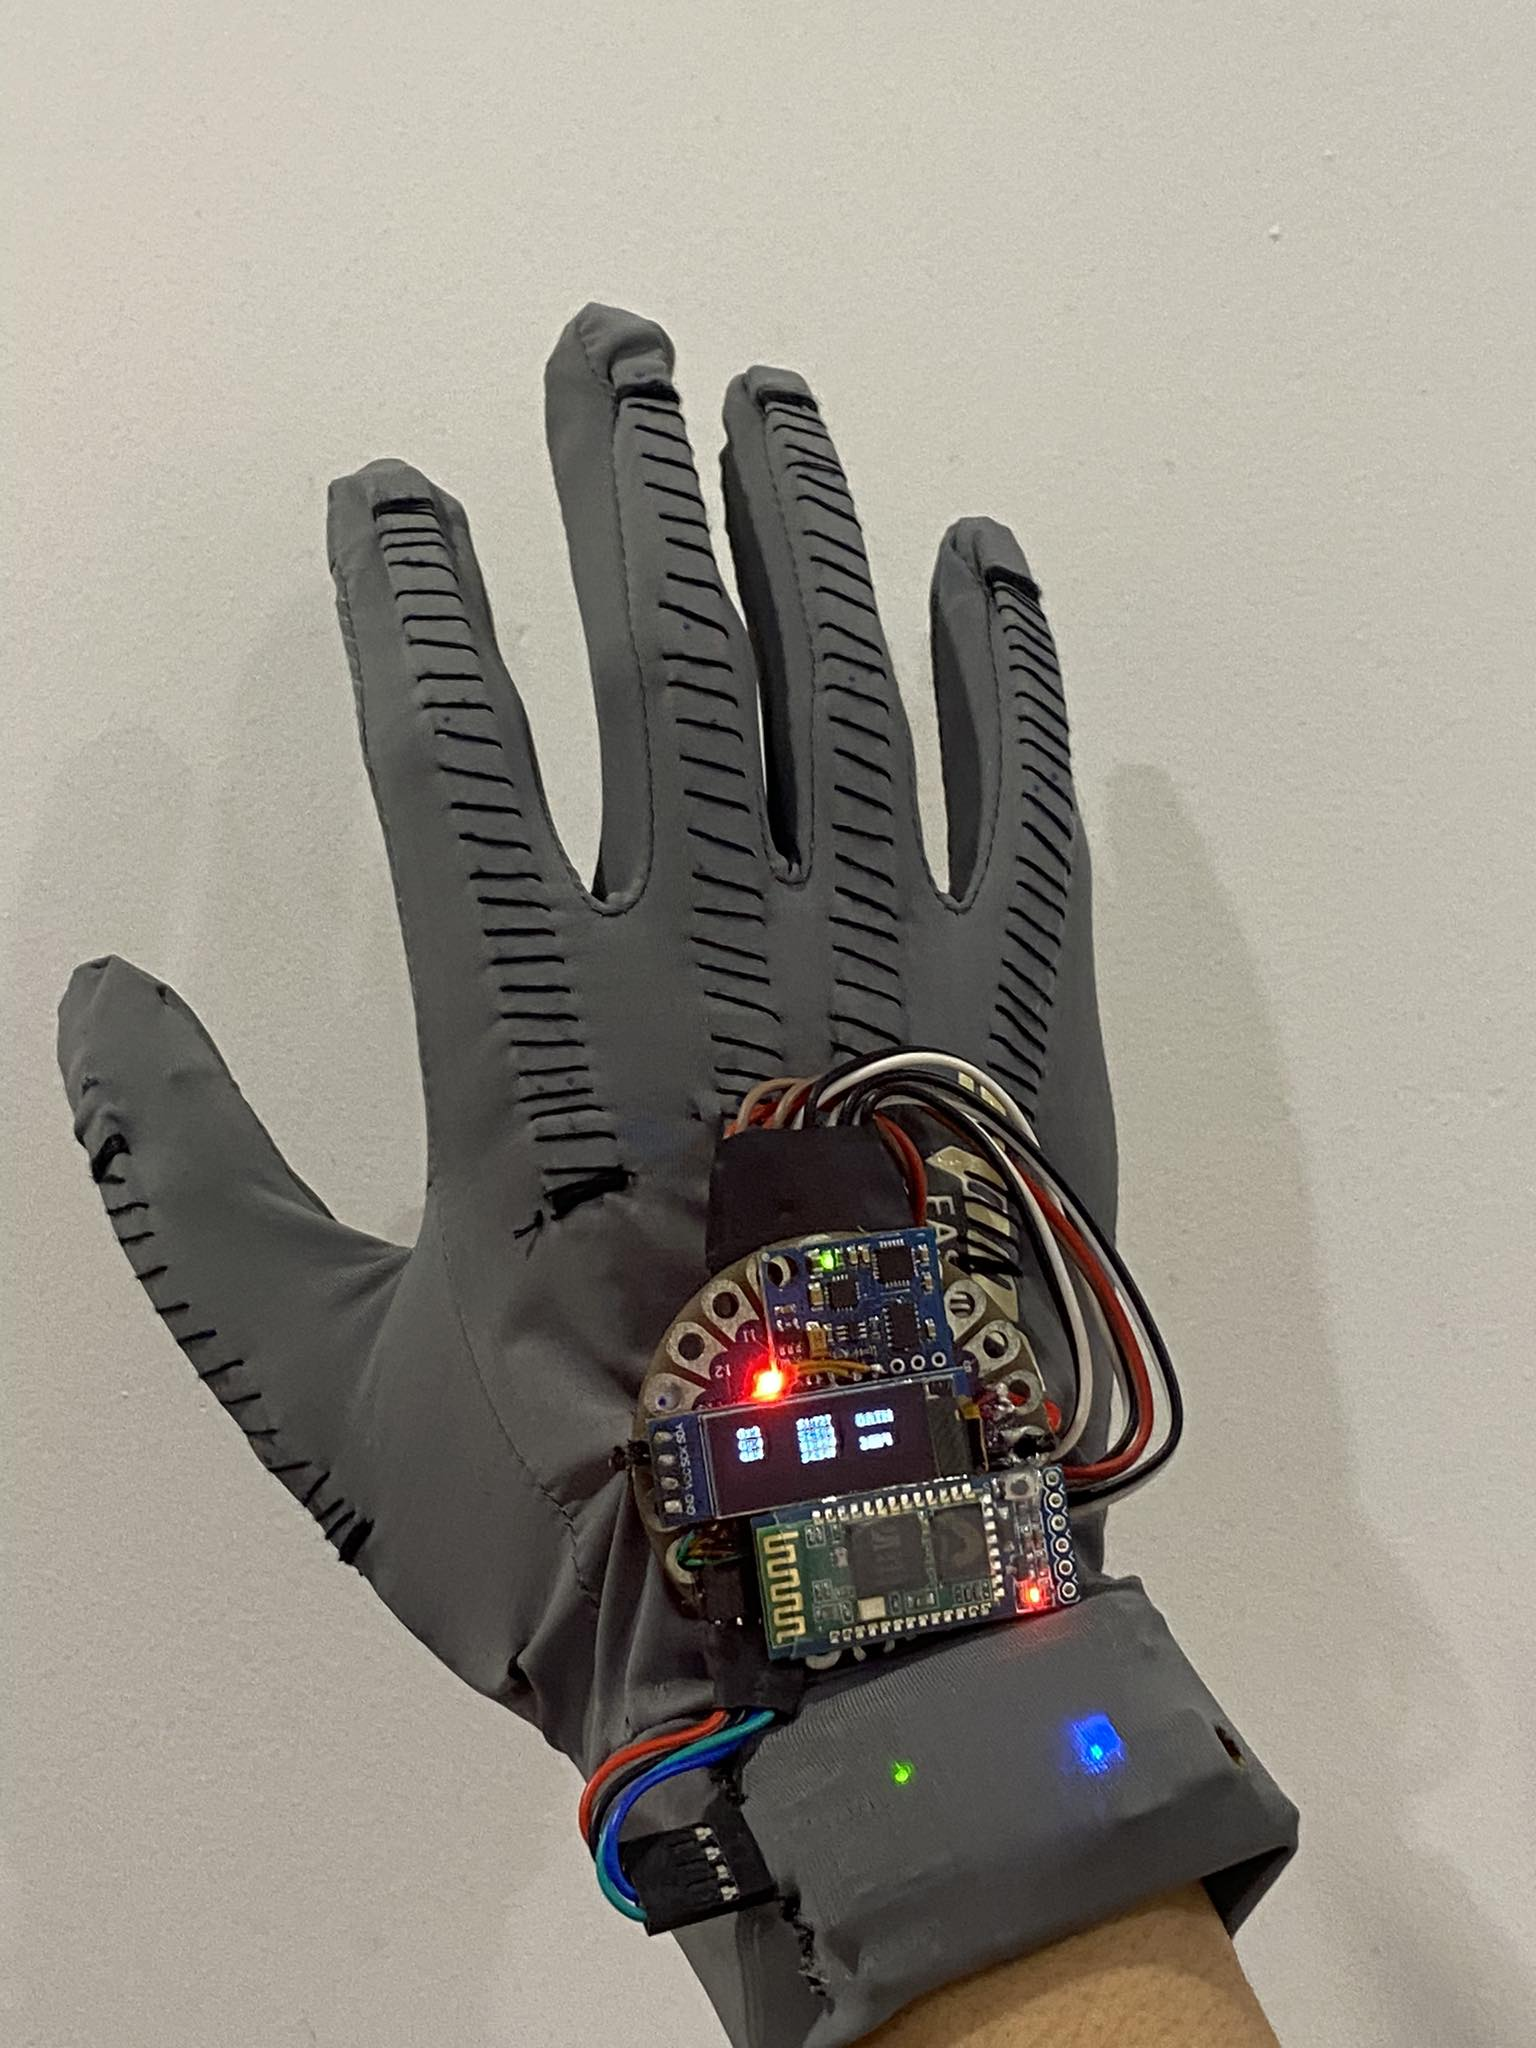
\includegraphics[width=\textwidth,height=\textheight,keepaspectratio]{Images/SystemImpl/full.jpg}
    \caption{Hình ảnh sau khi hoàn thiện}
    \label{fig:enter-label}
\end{figure}
\subsection{Xây dựng bộ dữ liệu}
Dữ liệu được thu thập từ module thu thập dữ liệu cử chỉ sau đó được lưu vào file text
\subsubsection{Dữ liệu được thu thập trên arduino}

Dữ liêu được gửi từ Arduino có 7 thành phần chính: 

\begin{lstlisting}
    gyro.readGyro(&ix,&iy,&iz); 
    ix = filter_gX.updateEstimate(ix);
    iy = filter_gY.updateEstimate(iy);
    iz = filter_gZ.updateEstimate(iz);
        readFlexSensor(flexSensor);
    flexSensor[0] = filter_flex0.updateEstimate(flexSensor[0]);
    flexSensor[1] = filter_flex1.updateEstimate(flexSensor[1]);
    flexSensor[2] = filter_flex2.updateEstimate(flexSensor[2]);
    flexSensor[3] = filter_flex3.updateEstimate(flexSensor[3]);
\end{lstlisting}

Các dữ liệu được gửi lần lượt là gia tốc trục x, gia tốc trục y, gia tốc trục z, và các tín hiệu analog 1,2,3,4. với flex 1,2 ( ngón trỏ và ngón cái) được nối song song với nhau sau đó nối tiếp đến A0, và các ngón còn lại được nối tuần tự

Đầu ra của tín hiệu được gửi qua blutetooth có dạng như sau: 
\begin{lstlisting}
"%lld\t%lld\t%lld\t%d\t%d\t%d\t%d\n"
\end{lstlisting}
 
dữ liệu được gửi với mỗi 10ms một lần

\begin{figure}[H]
    \centering
    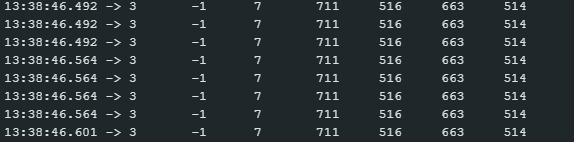
\includegraphics[width=\textwidth,height=\textheight,keepaspectratio]{Images/SystemImpl/data.png}
    \caption{Dạng dữ liêu được gửi}
    \label{fig:enter-label}
\end{figure}

\subsubsection{Dữ liệu nhận được từ gateway}
\begin{lstlisting}
SERIAL_PORT = 'COM5'
SERIAL_RATE = 38400
label = 14
DATA_FILE_NAME = './datatrain1/trainx_'+str(label)+'.txt'  # Specify the output file name
LABEL_FILE_NAME = './datatrain1/trainy_'+str(label)+'.txt'  # Specify the output file name
DATA_TEST_FILE_NAME = './datatrain1/testx_'+str(label)+'.txt'  # Specify the output file name
LABEL_TEST_FILE_NAME = './datatrain1/testy_'+str(label)+'.txt'  # Specify the output file name
test_counter = 300
queue_size = 240
windowSlide = 60
training_times = 200
testing_times = 40
\end{lstlisting}
\begin{itemize}

\item\textbf{SERIAL\_PORT} là cổng kết nối với thiết bị
Sau khi kết nối với bluetooth với arduino, kiểm tra cổng COM đã kết nối bằng cách mở phần mềm arduino

\begin{figure}[H]
    \centering
    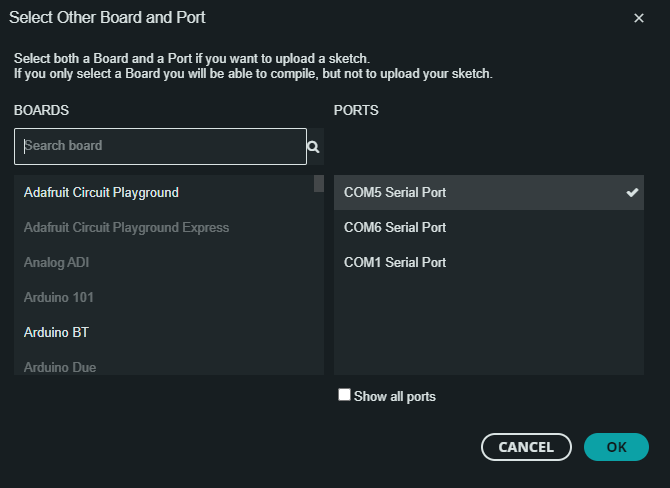
\includegraphics[width=\textwidth,height=\textheight,keepaspectratio]{Images/SystemImpl/checkcomport.png}
    \caption{kiểm tra các cổng com đang mở}
    \label{fig:enter-label}
\end{figure}

Ví dụ trong bài luận văn này là cổng 5 \\

\item\textbf{SERIAL\_RATE} ở đây là baudraute khi khởi tạo ở arduino, ở đây module bluetooth HC-05 sử dụng 38400 để đảm bảo thời gian trễ thấp nhất khi một frame dữ liệu được gửi qua\\

\item\textbf{label} là nhãn của dữ liệu khi được train,nhãn này được định nghĩa ở file config và readme như sau \\

\begin{longtblr}[
  caption = {File readme mô tả hành động được thu nhập và gắn nhãn},
]{
  width = \linewidth,
  colspec = {Q[404]Q[521]},
  hlines,
  vlines,
}
label 0          & hành động nắm tay  \\
label 1      & hành động tạm biệt ( hành động chậm)\\
label 2& hành động tạm biệt ( hành động chậm)\\                              
label 3 &chỉ vào bản thân (ngón cái đưa lên)\\
label 4 &không biết ( bàn tay xòe thẳng và xoay quanh trục ngón giữa)\\
label 5 &trạng thái nghỉ\\
label 6 &chỉ ra ngoài ( chỉ một ngón trỏ đưa lên) \\
label 7 &hành động đi bộ ( ngón giữa và ngón trỏ)\\
label 8 &ngón trỏ chỉ xuống đất và xoay vòng \\
label 9 &đùa giỡn ( ngón trỏ và ngón giữa co giãn cùng một lúc) \\
label 10 &chỉ tại đây (ngón cái và ngón giữa chỉ xuống, ngón cái đưa lên )\\
label 11 &hành động xin chào ( hành động nhanh ) \\
label 12 &giới thiệu tên \\
label 13 &thể hiện trạng thái vui vẻ ( bàn tay xòe thẳng và xoay vòng quanh cổ tay ) \\
label 14 &hành động gặp nhau ( ngón trỏ chỉ lên, các ngón còn lại co )\\
\end{longtblr}

\begin{longtblr}[
  caption = {File config là các đoạn text được chuyển sang giọng nói},
]{
  width = \linewidth,
  colspec = {Q[404]Q[521]},
  hlines,
  vlines,
}
Giữ & ~0\\
Tạm Biệt& ~1\\
Tốt lắm&~2\\
Tôi&~3\\
Không biết&~4\\
-&~5\\
Bạn&~6\\
Đi bộ&~7\\
Xung quanh&~8\\
Đùa thôi&~9\\
Tại đây&~10\\
Xin chào&~11\\
Tên là Chánh (điều chỉnh để phát ra tên như mong muốn)&~12\\
Rất vui&~13\\
Gặp&~14
\end{longtblr}

\item\textbf{DATA\_FILE\_NAME}: nơi lưu trainx\\
\item\textbf{LABEL\_FILE\_NAME}: nơi lưu trainy\\
\item\textbf{DATA\_TEST\_FILE\_NAME}: nơi lưu testx\\
\item\textbf{LABEL\_TEST\_FILE\_NAME}: nơi lưu testy\\
\item\textbf{test\_counter}: số lần test dữ liệu, được định tính trước khi bắt đầu thu thập \\
\item\textbf{queue\_size}: một frame dữ liệu để gắn nhãn cho frame đó\\
\item\textbf{windowSlide}: cửa số trượt, một lượng dữ liệu một để thêm vào một frame, trùng lặp với frame trước đó được tính bằng $queue\_size - windowSlide$
\item\textbf{training\_times}: số frame dữ liệu được ghi vào file train
\item\textbf{testing\_times}: số frame dữ liệu được ghi vào file test
\end{itemize}

Tiến hành thu thập dữ liệu với các động tác tay được định nghĩa như ở file readme
\begin{figure}[H]
    \centering
    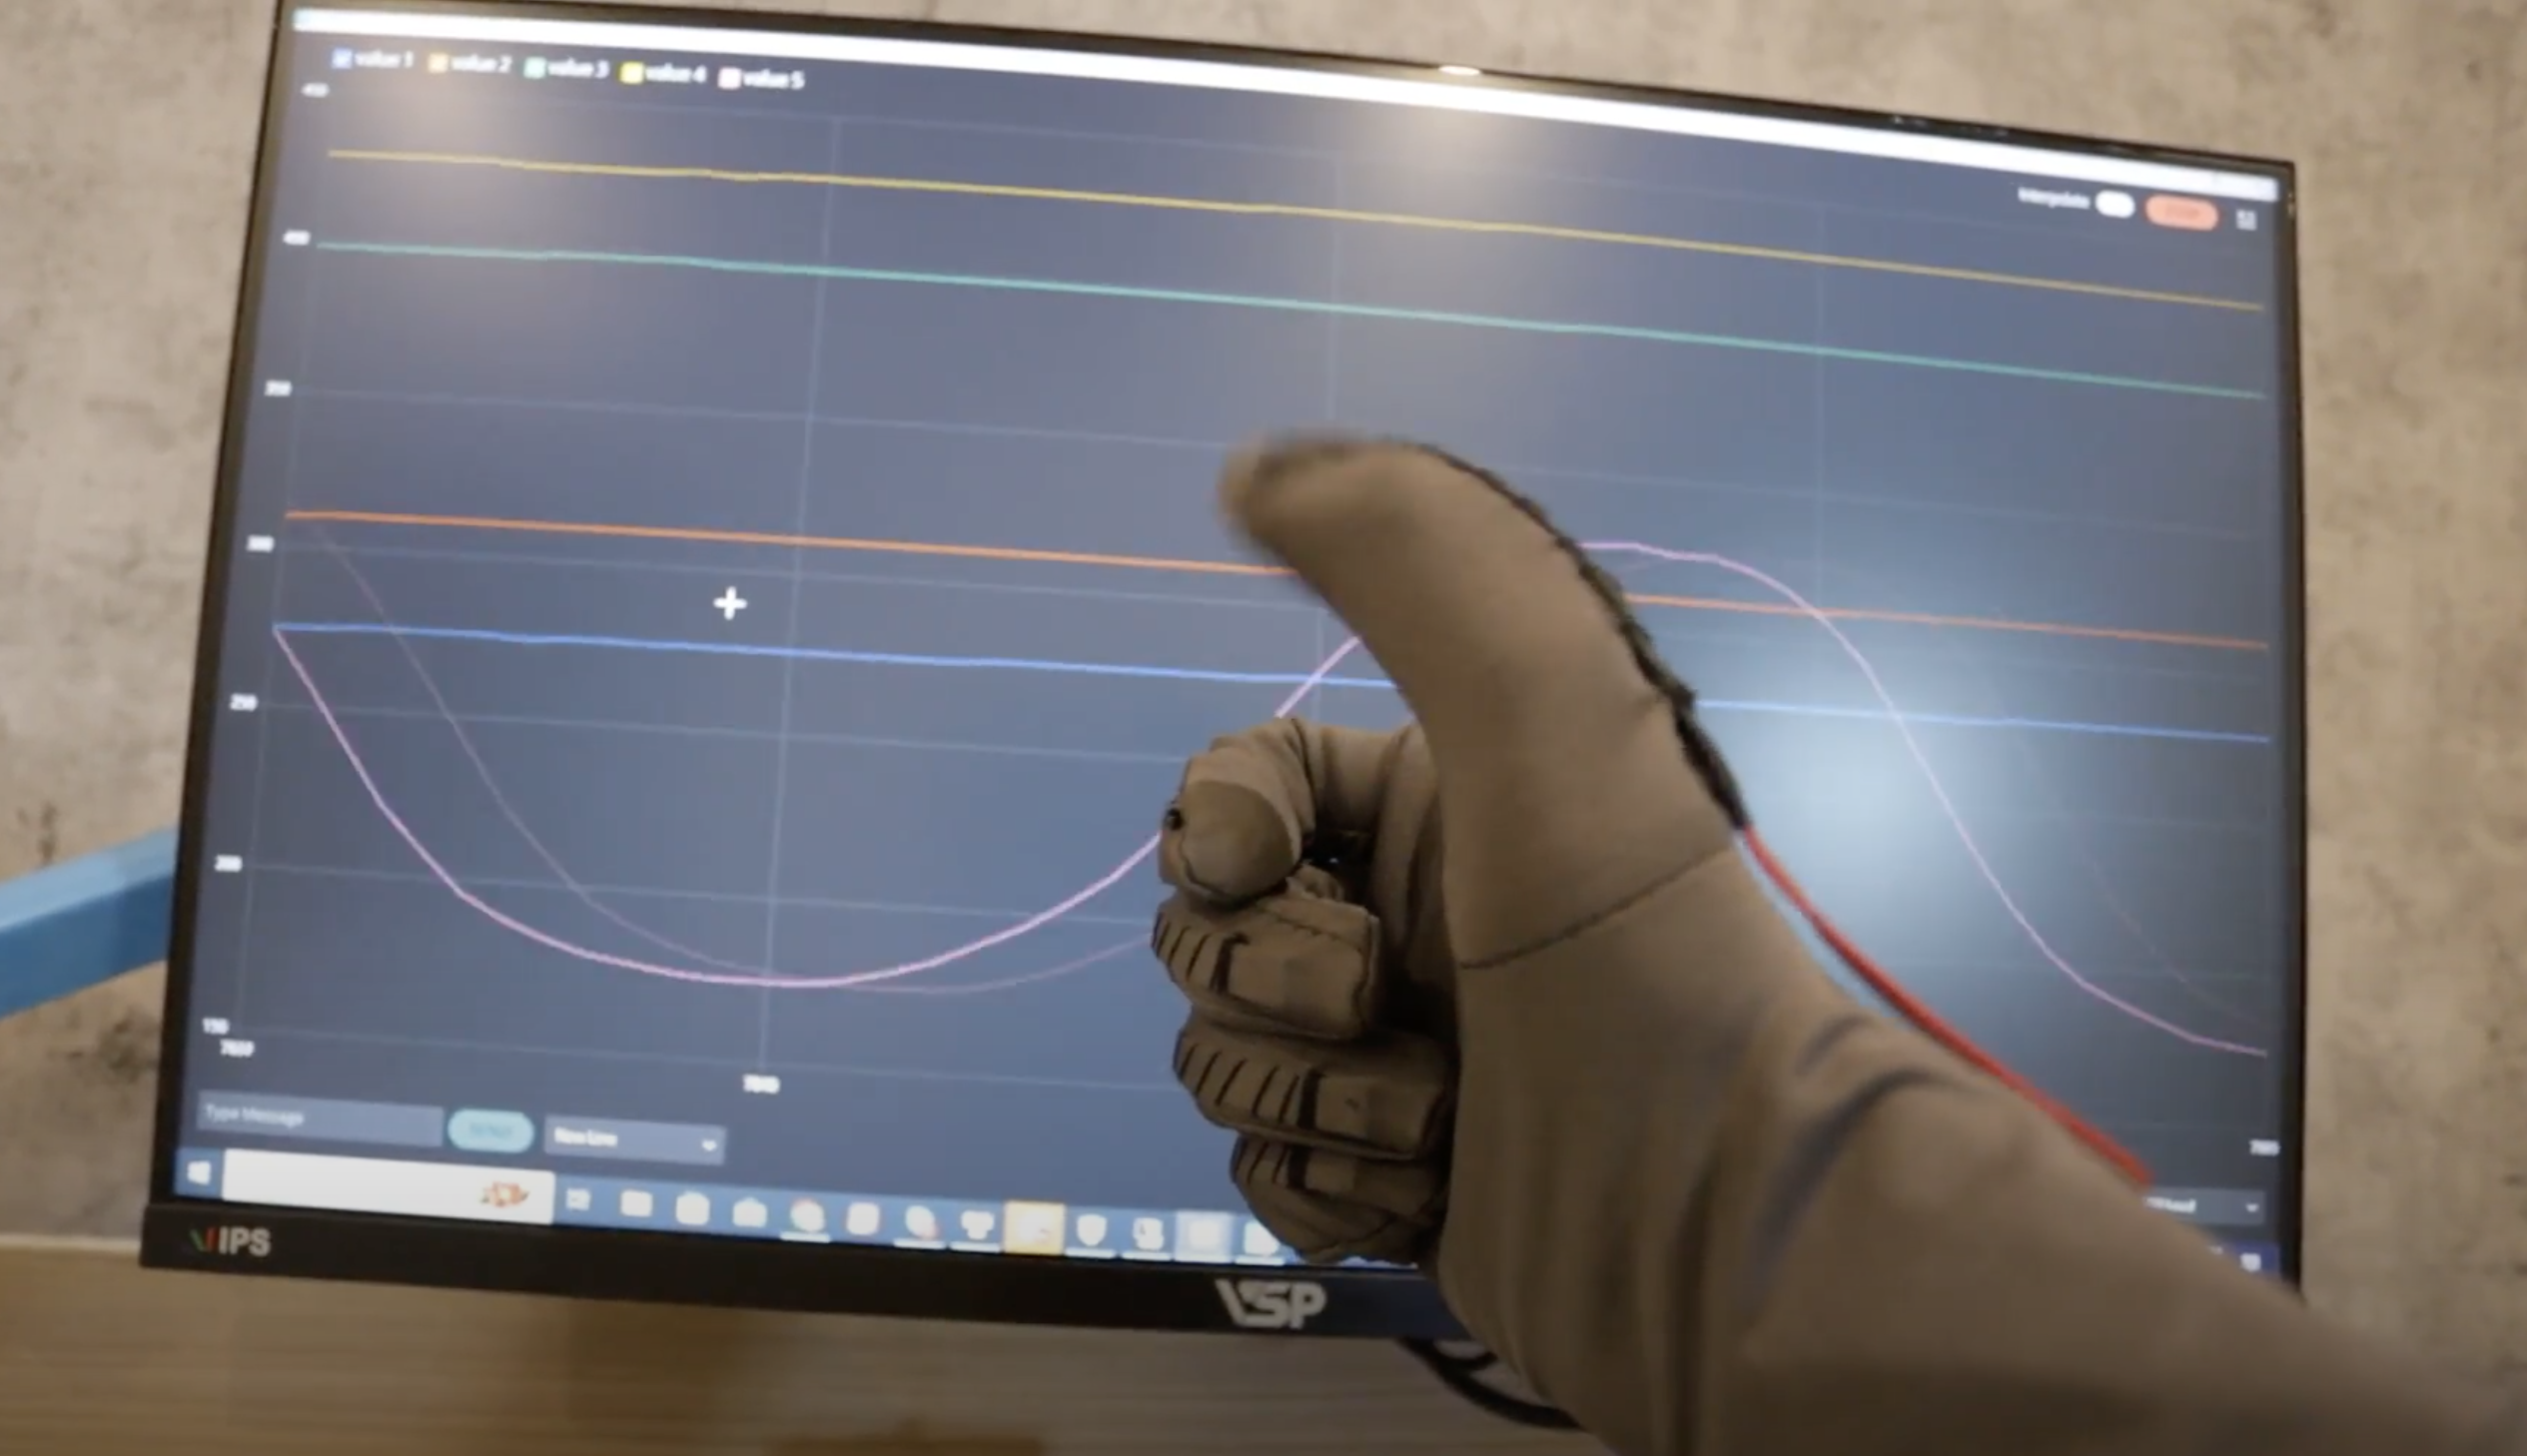
\includegraphics[width=10cm]{Images/SystemImpl/readdt_result_1.png}
    \centering
    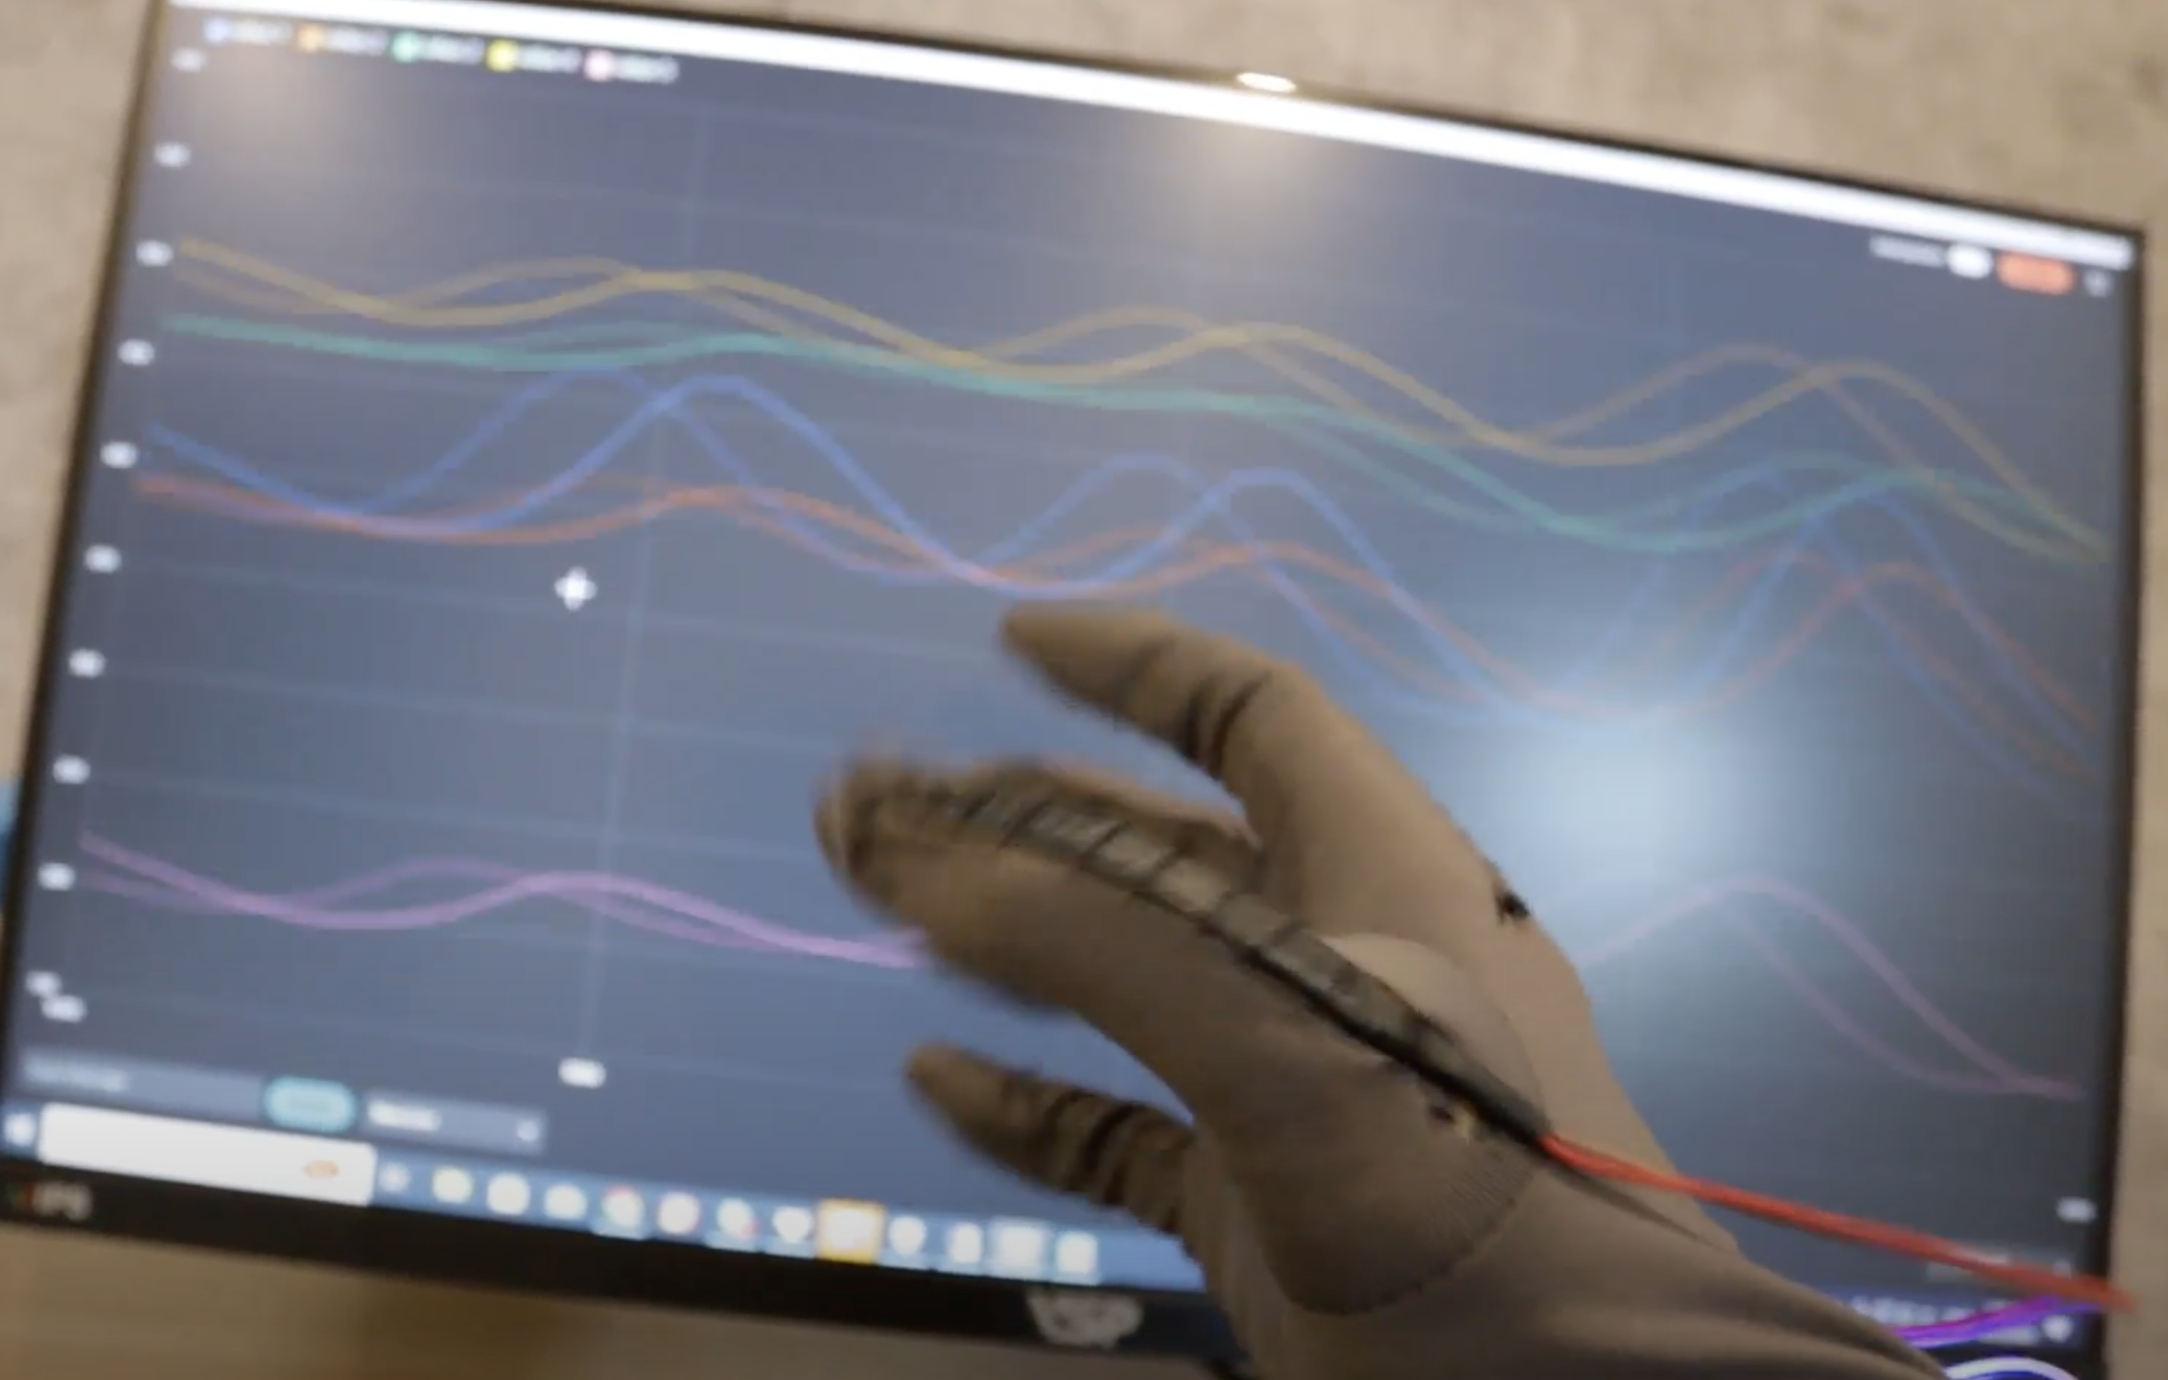
\includegraphics[width=10cm]{Images/SystemImpl/readdt_result_2.png}
\caption{Quá trình lấy dữ liệu}
\end{figure}

Các file data được lưu có kích thước cho một hành động như sau 
\begin{itemize}
    \item Một hàng có 240*7 cột dữ liệu
    \item Có tổng cộng 200 hàng dữ liệu cho file train và 20 cho trainy 
\end{itemize}
\newpage
\subsection{Định dạng data trước khi đưa vào học máy}
\begin{lstlisting}
line = next(testx).strip().split()
                if len(line) >= 1680:
                    for i in range(240):
                        x1.append(int(line[i]))
                        x2.append(int(line[i + 240]))
                        x3.append(int(line[i + 480]))
                        x4.append(int(line[i + 720]))
                        x5.append(int(line[i + 960]))
                        x6.append(int(line[i + 1200]))
                        x7.append(int(line[i + 1440]))
                else:
                    print("Error test data.")
                x1 = array(x1)
                x2 = array(x2)
                x3 = array(x3)
                x4 = array(x4)
                x5 = array(x5)
                x6 = array(x6)
                x7 = array(x7)
                line_dataset = dstack([x1, x2, x3, x4, x5, x6, x7]) 
                line_dataset = line_dataset.reshape(1,240,7)
                testx_data.append(line_dataset)
\end{lstlisting}

Có hai loại tín hiệu chính trong dữ liệu gốc: gia tốc và flexsensor
Gia tốc có 3 trục dữ liệu, flexsensor có 4 trục dữ liệu
mỗi loạt dữ liệu được ghi với thời gian là 2.4 giây
tương đương với 240 bước thời gian. Các cửa sổ dữ liệu này tương ứng với các cửa sổ đặc trưng đã được tạo ra trước đó. Điều này có nghĩa là một hàng dữ liệu có (240 * 7), tức là 1680 phần tử.

Dữ liệu sau khi được tải từ file text, sau đó được phân chia thành từng frame dữ liệu:\\
Mỗi frame dữ liệu có các tính chất như sau:
\begin{itemize}
\item Mỗi cột dữ liệu được ghi 240 lần 
\item Có tổng cộng 7 cột dữ liệu tương ứng với 7 feature của một frame

\end{itemize}
Có thể thấy hàm reshape sẽ đảm nhận việc đó
\newpage
\subsection{Xây dựng mô hình}




Sau khi train thành công dựa trên bộ dữ liệu, các tham số của mô hình được lưu vào file h5. file này được sử dụng để dự đoán các hành động











\newpage
%%%%%%%%%%%%%%%%%%%%%%%%%%%%%%%%%
\section{Các phương pháp cải tiến}
\subsection{Sliding Window}
\subsection{Khắc phục vấn đề mất dữ liệu}
\subsection{Cải thiện chất lượng mô hình}
\subsubsection{Mô hình với Deep Convolution và Self-Attention}

Trong đề tài trước, mô hình học máy được sử dụng khá thô sơ và đơn giản, bao gồm các thành phần chính: một lớp \textit{LSTM}, một lớp \textit{Dropout}, một lớp \textit{Flatten}, và hai lớp \textit{Dense}. 

\begin{figure}[H]
    \centering
    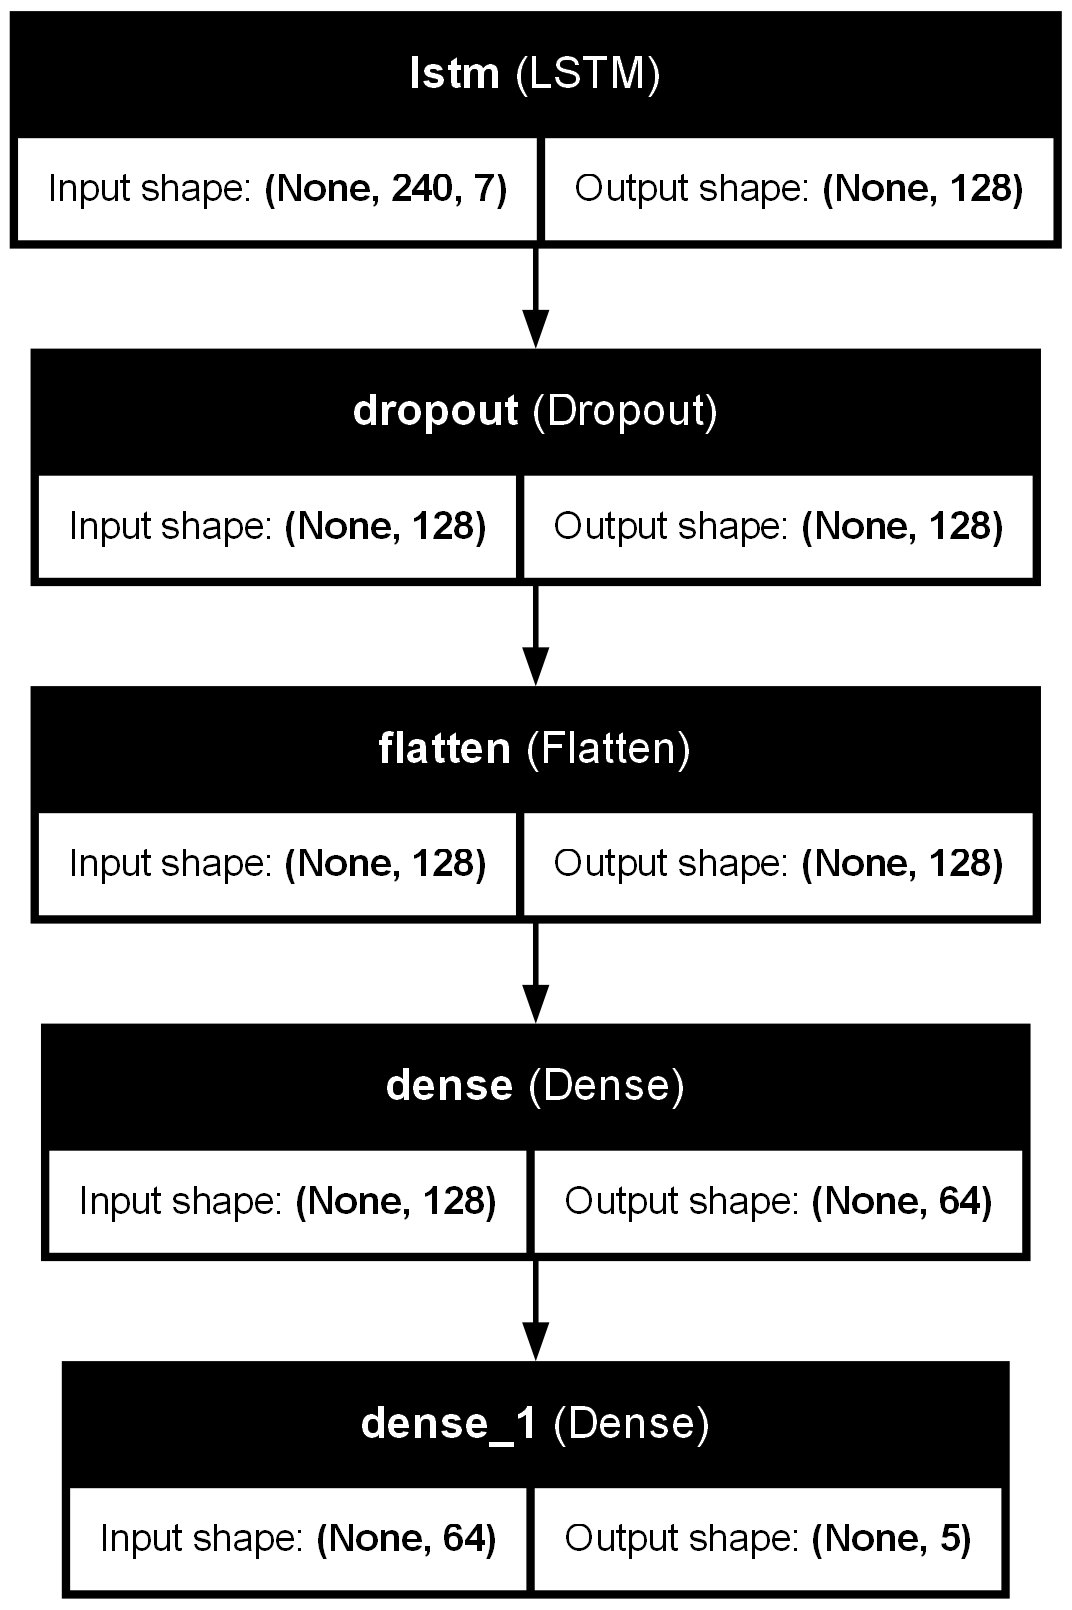
\includegraphics[width=0.5\linewidth]{Images/Improved methods/old_model_plot.png}
    \caption{Cấu trúc mô hình cũ}
    \label{fig:old-model}
\end{figure}

Kết quả đạt được từ mô hình này vẫn chưa thực sự khả quan. Để cải thiện chất lượng đầu ra, cần thực hiện hai bước quan trọng:
\begin{itemize}
    \item \textbf{Gia tăng kích thước tập dữ liệu}: Mở rộng và đa dạng hóa dữ liệu đầu vào.
    \item \textbf{Nâng cấp mô hình}: Sử dụng kiến trúc học máy hiệu quả hơn để khai thác triệt để thông tin từ dữ liệu.
\end{itemize}

Trong đề tài này, nhóm đề xuất một mô hình cải tiến, dựa trên kiến trúc được giới thiệu trong bài báo \textit{"Self-Attention-Based Deep Convolution LSTM Framework for Sensor-Based Badminton Activity Recognition"} (\href{https://doi.org/10.3390/s23208373}{DOI: 10.3390/s23208373}). Mô hình này kết hợp:
\begin{enumerate}
    \item \textbf{Mạng nơ-ron tích chập (CNN)}: Chiết xuất các đặc trưng cục bộ từ dữ liệu đầu vào.
    \item \textbf{Mạng nơ-ron hồi quy (LSTM)}: Nắm bắt các phụ thuộc dài hạn trong dữ liệu.
    \item \textbf{Cơ chế Self-Attention}: Tập trung vào các phần quan trọng nhất của dữ liệu.
\end{enumerate}

Mô hình đề xuất bao gồm các thành phần chính sau:
\begin{itemize}
    \item \textbf{Lớp CNN}: Chiết xuất các đặc trưng cục bộ từ dữ liệu đầu vào.
    \item \textbf{Lớp LSTM}: Nắm bắt và lưu giữ các thông tin phụ thuộc dài hạn trong chuỗi thời gian.
    \item \textbf{Cơ chế Self-Attention}: Xác định và tập trung vào các đặc trưng quan trọng nhất trong dữ liệu, cải thiện hiệu quả học hỏi của mô hình.
\end{itemize}

\begin{figure}[H]
    \centering
    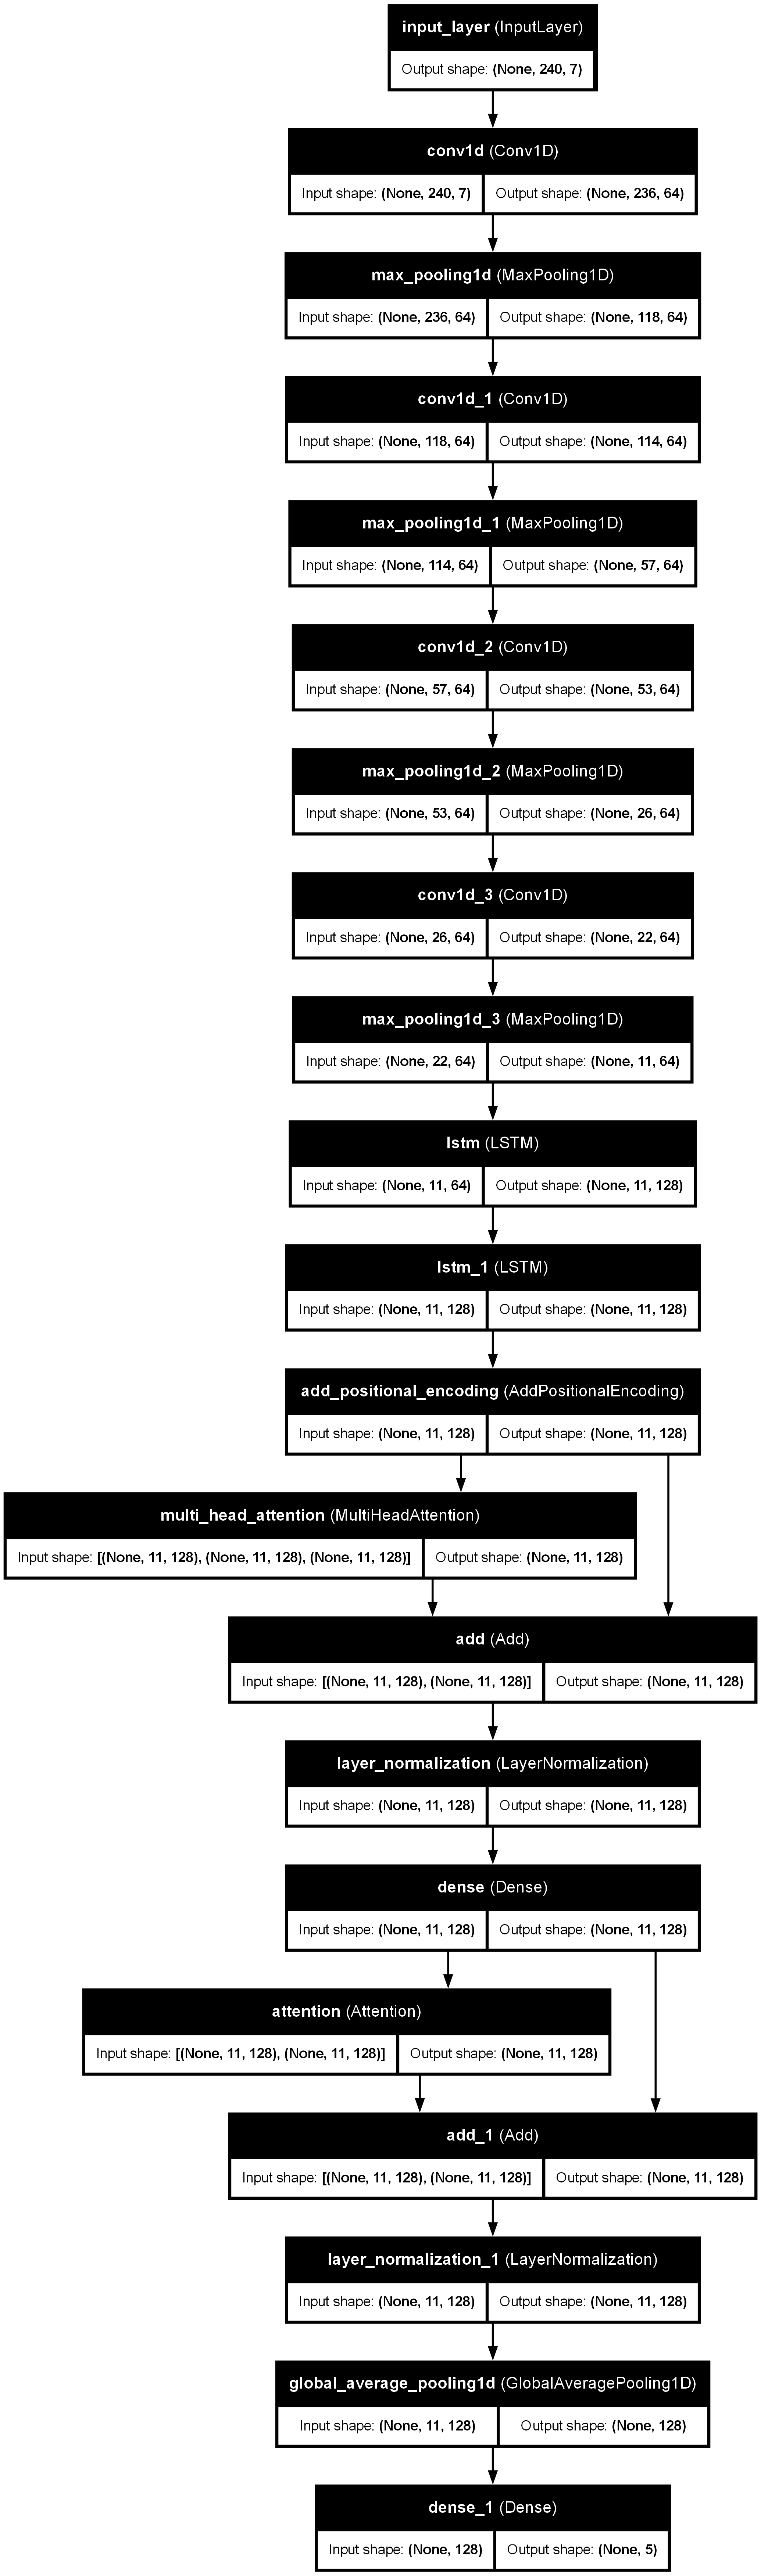
\includegraphics[width=0.4\linewidth]{Images/Improved methods/new_model_plot.png}
    \caption{Mô hình mới}
    \label{fig:new-model}
\end{figure}


\noindent
Cơ chế \textit{Self-Attention} đóng vai trò then chốt trong việc nâng cao hiệu suất của mô hình. Nó cho phép mô hình tự động:
\begin{itemize}
    \item Phân tích toàn bộ dữ liệu đầu vào.
    \item Tập trung vào những đặc trưng mang tính quyết định.
\end{itemize}

Nhờ vậy, mô hình có thể đạt được độ chính xác cao hơn trong việc dự đoán các hành động theo chuỗi thời gian.

\subsection{Làm giàu dữ liệu}
\subsubsection{Data Augmentation}

Trong học máy, \textit{Data Augmentation} là một kỹ thuật quan trọng giúp mở rộng tập dữ liệu hiện có bằng cách tạo ra các biến thể mới của dữ liệu. Điều này không chỉ cải thiện tính đa dạng của dữ liệu mà còn giúp mô hình giảm thiểu hiện tượng quá khớp (\textit{overfitting}) và học được nhiều đặc trưng tổng quát hơn. Dưới đây là một số kỹ thuật được áp dụng:

\begin{enumerate}

\item \textbf{Jittering}: 
\begin{itemize}
\item \textbf{Mô tả}: Thêm nhiễu ngẫu nhiên vào dữ liệu. Jittering có thể được thực hiện bằng cách thêm một lượng nhỏ nhiễu Gaussian vào mỗi điểm dữ liệu. Điều này giúp mô hình ít bị ảnh hưởng bởi nhiễu trong dữ liệu thực tế và tăng khả năng kháng nhiễu của mô hình.
\item \textbf{Lợi ích}: 
\begin{itemize}
\item Giúp mô hình trở nên mạnh mẽ hơn trước các biến động nhỏ trong dữ liệu thực tế.
\item Tăng khả năng tổng quát hóa bằng cách làm cho dữ liệu đầu vào đa dạng hơn.
\end{itemize}
\end{itemize}

\item \textbf{Scale}: 
\begin{itemize}
\item \textbf{Mô tả}: Thay đổi tỷ lệ của dữ liệu. Scale được thực hiện bằng cách nhân mỗi điểm dữ liệu với một hệ số tỷ lệ ngẫu nhiên.
 \item \textbf{Lợi ích}:
\begin{itemize}
\item Giúp mô hình học được các đặc trưng ở các mức độ hoặc tỉ lệ khác nhau.
 \item Phù hợp với các bài toán mà dữ liệu có sự biến thiên về kích thước, chẳng hạn như tín hiệu sinh lý.
\end{itemize}
 \end{itemize}

\item \textbf{Magnitude Warp}: 
\begin{itemize}
\item \textbf{Mô tả}: Biến dạng biên độ của dữ liệu theo một hàm phi tuyến. Magnitude Warp có thể được thực hiện bằng cách áp dụng một hàm phi tuyến, chẳng hạn như hàm sin hoặc hàm mũ, cho biên độ của dữ liệu.
\item \textbf{Lợi ích}:
\begin{itemize}
\item Tạo ra các biến thể tín hiệu thực tế hơn, đặc biệt phù hợp với các bài toán liên quan đến chuỗi thời gian.
\item Làm phong phú tập dữ liệu và giúp mô hình ít phụ thuộc vào các dạng tín hiệu cụ thể.
 \end{itemize}
\end{itemize}

\item \textbf{Shift}: 
 \begin{itemize}
 \item \textbf{Mô tả}: Dịch chuyển dữ liệu theo thời gian. Shift được thực hiện bằng cách dịch chuyển toàn bộ chuỗi thời gian sang trái hoặc phải một khoảng thời gian ngẫu nhiên.
 \item \textbf{Lợi ích}:
\begin{itemize}
\item Tăng khả năng chống lại sự thay đổi vị trí trong dữ liệu, chẳng hạn như các tín hiệu không đồng bộ.
\item Giúp mô hình học được các đặc trưng không bị phụ thuộc vào vị trí cụ thể.
\end{itemize}
\end{itemize}

\end{enumerate}

Để tăng cường dữ liệu huấn luyện, nhóm đã xây dựng một script Python để áp dụng các kỹ thuật Data Augmentation đã đề cập ở trên. Script này nhận dữ liệu gốc làm đầu vào và tạo ra các phiên bản biến đổi của dữ liệu bằng cách sử dụng các kỹ thuật Jittering, Scale, Magnitude Warp và Shift.

Mỗi kỹ thuật Data Augmentation được áp dụng riêng biệt, tạo ra một phiên bản mới của tập dữ liệu với cùng kích thước với tập dữ liệu gốc. Do đó, sau khi áp dụng cả bốn kỹ thuật, nhóm thu được một tập dữ liệu mới có kích thước gấp 5 lần tập dữ liệu ban đầu (bao gồm cả dữ liệu gốc). 

Việc tăng kích thước tập dữ liệu huấn luyện thông qua Data Augmentation giúp cải thiện khả năng tổng quát hóa của mô hình, giảm thiểu hiện tượng overfitting và tăng cường độ chính xác của mô hình trên dữ liệu mới.
\subsubsection{Transfer learning}
Một cách cải thiện hiệu suất của mô hình là sử dụng \textit{Transfer learning}. Transfer learning là một kỹ thuật học máy mà mô hình được huấn luyện trước trên một tập dữ liệu lớn và sau đó được sử dụng để giải quyết một bài toán mới. Nhóm sử dụng một tập dữ liệu có tên là "DU-ASL-DATA-GLOVE-DB" được công bố trên trang web \href{https://figshare.com/articles/dataset/ASL-Sensor-Dataglove-Dataset_zip/20031017?file=35776586}{Figshare}. Tập dữ liệu này chứa dữ liệu về ngôn ngữ ký hiệu Mỹ (ASL) được thu thập từ cảm biến găng tay thông minh.

\begin{itemize}
    \item \textbf{Tổng quan:} Đây là một tập dữ liệu được thu thập bởi 1 nhóm sinh viên chuyên ngành kỹ thuật sinh học tại Ấn Độ, họ thu thập dữ liệu từ 25 người khác nhau (19 nam và 6 nữ). Mỗi người thực hiện 40 cử chỉ khác nhau (26 cử chỉ trong bảng chữ cái và 14 từ). Dữ liệu được thu thập từ cảm biến với tần số lấy mẫu 100Hz và mỗi cử chỉ có thời lượng 1.5 giây và được thực hiện 10 lần cho mỗi đối tượng.
    \item \textbf{Thông tin phần cứng:} Dữ liệu được thu thập từ 5 cảm biến flex 2.2 inch SEN-10264 và 1 cảm biến IMU MPU6050.
    \item \textbf{Tổ chức dữ liệu:} Dữ liệu được lưu trong 25 thư mục được đánh số từ 001 đến 025, mỗi thư mục chứa dữ liệu của một người. Mỗi thư mục chứa 40 file csv tương ứng với 40 cử chỉ khác nhau. Mỗi file csv chứa dữ liệu của 10 lần thực hiện cử chỉ. 
    \item \textbf{Tiền xử lý:} Dữ liệu cần được xử lý để có thể phu hợp với mô hình của nhóm. Mô hình học máy nhóm sử dụng yêu cầu dữ liệu đầu vào phải có timestep là 250 và số chiều là 7. Do đó nhóm cần thực hiện 2 bước tiền xử lý chính:
    \begin{itemize}
        \item \textbf{Thay đổi tập dữ liệu} Vì tín hiệu ở cột thứ 4 được tính bằng tổng tín hiệu của cảm biến từ ngón áp út và ngón út, nhóm cần phải tính lại giá trị của cột này bằng cách tính tổng điện trở của f4 và f5 trong dataset. Nhóm cũng chỉ sử dụng giá trị từ flex sensor và cảm biến góc quay vì thiết bị không có cảm biến gia tốc.
        \item \textbf{Upscaling dữ liệu:} Dữ liệu được thu thập với tần số lấy mẫu 100Hz với thời gian thực hiện cử chỉ là 1.5 giây. Điều đó có nghĩa là dữ liệu thu được có số lượng timestep là 150. Để phù hợp với mô hình nhóm sử dụng, nhóm cần phải upscaling dữ liệu lên 250 timestep. Kỹ thuật upscaling được sử dụng là nội suy tuyến tính.
    \end{itemize}
    \begin{figure}
        \centering
        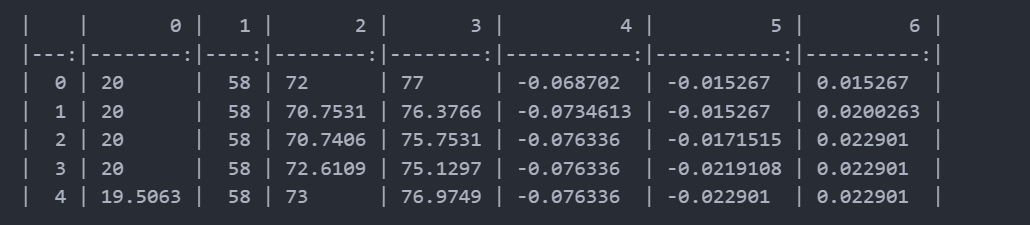
\includegraphics[width=0.8\linewidth]{Images/Improved methods/transfer_learning.png}
        \caption{Dữ liệu sau khi chỉnh sửa}
        \label{fig:interpolation}
    \end{figure}
    \item \textbf{Huấn luyện mô hình:} Mô hình được sử dụng là mô hình cải tiến mà nhóm đã giới thiệu ở trên. Mô hình được huấn luyện trên tập dữ liệu ASL. Weight của mô hình được lưu lại và sử dụng cho việc huấn luyện mô hình trên tập dữ liệu của nhóm.
\end{itemize}
\subsubsection{Sinh dữ liệu từ TimeGAN}

\newpage
%%%%%%%%%%%%%%%%%%%%%%%%%%%%%%%%%
\section{Kết quả của các kỹ thuật cải tiến}
\subsection{Mô hình cải tiến}
Có thể thấy được cả hai mô hình đều có thể hội tụ sao 10 epoch, nhưng mô hình cải tiến hội tụ nhanh hơn và có loss thấp hơn so với mô hình cũ. Điều này có thể thấy rõ ở hình \ref{fig:loss_model}. Mô hình cải tiến có loss thấp hơn mô hình cũ sau 10 epoch. Điều này có thể hiểu là mô hình cải tiến học nhanh hơn và hiệu quả hơn so với mô hình cũ.

\begin{figure}[H]
    \centering
    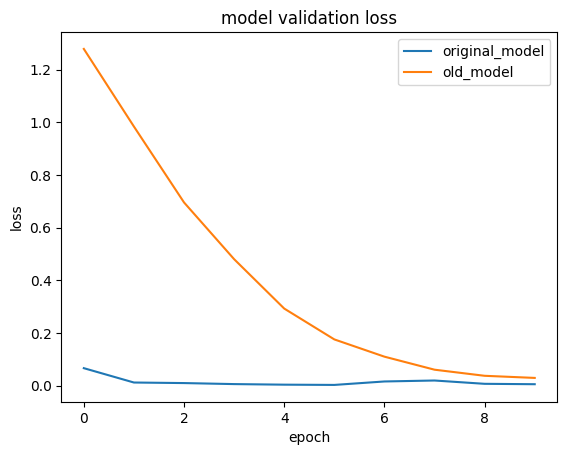
\includegraphics[width=0.8\textwidth]{Images/Improvement results/old_new_loss.png}
    \caption{Loss của cả hai mô hình }
    \label{fig:loss_model}
\end{figure}

Điều này có thể thấy rõ hơn ở confusion matrix của cả hai mô hình ở trên tập test. Mô hình cải tiến có thể dự đoán chính xác đa số các mẫu trong tập test trong khi mô hình cũ dự đoán sai một số mẫu trong tập test.

\begin{figure}[H]
    \centering
    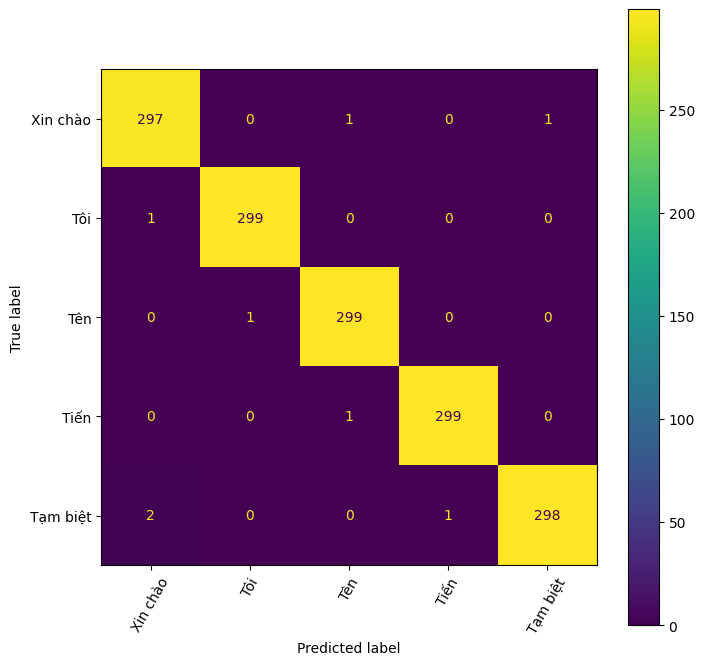
\includegraphics[width=0.8\textwidth]{Images/Improvement results/new_confusion_matrix.png}
    \caption{Confusion matrix của mô hình mới}
    \label{fig:confusion_matrix_new}
\end{figure}

\begin{figure}[H]
    \centering
    \includegraphics[width=0.8\textwidth]{Images/Improvement results/old_confusion_matrix.png}
    \caption{Confusion matrix của mô hình cũ}
    \label{fig:confusion_matrix_old}
\end{figure}

Không những vậy mô hình cũng có confidence trung bình cho những mẫu đoán đúng cao hơn so với mô hình cũ. Điều này có thể thấy rõ ở hình \ref{fig:confidence_model}. Mô hình cải tiến có confidence trung bình cho những mẫu đoán đúng cao hơn mô hình cũ. 

\begin{figure}[H]
    \centering
    \includegraphics[width=0.8\textwidth]{Images/Improvement results/old_new_confidence.png}
    \caption{Confidence của cả hai mô hình}
    \label{fig:confidence_model}
\end{figure}

Kiểm nghiệm thực tế cũng cho thấy mô hình cải tiến hoạt động tốt hơn so với mô hình cũ. Mô hình cải tiến có thể dự đoán chính xác hơn 90\%  trong khi mô hình cũ chỉ có thể dự đoán chính xác khoảng 70\% và cũng như có confidence cao hơn trong các lần dự đoán.

\subsection{Làm giàu dữ liệu}
\subsubsection{Data augmentation}
Nhóm chọn 4 kỹ thuật làm giàu dữ liệu là: Jitter, Shift, Scale và Magnitude Warp.

\begin{figure}[H]
    \centering
    \includegraphics[width=1\textwidth]{Images/Improvement results/data_augmentation.png}
    \caption{Data augmentation}
    \label{fig:data_augmentation}
\end{figure}

Với mỗi kỹ thuật làm giàu dữ liệu, nhóm đã ghép 2 kỹ thuật lại với nhau để tạo ra 6 cặp kỹ thuật làm giàu dữ liệu. 
Sau cùng dữ liệu có kích thước gấp 10 lần dữ liệu ban đầu.

\begin{figure}[H]
    \centering
    \includegraphics[width=0.8\textwidth]{Images/Improvement results/data_augmentation_loss.png}
    \caption{Loss của các kỹ thuật làm giàu dữ liệu}
    \label{fig:data_augmentation_loss}
\end{figure}



Nhìn chung kết quả của các kỹ thuật đều giúp mô hình hội tụ nhanh hơn khi sử dụng tập dữ liệu ban đầu. Bởi vì mô hình mới với dữ liệu ban đầu đã làm rất tốt nên việc làm giàu dữ liệu không thể hiện rõ ở mặt độ chính xác của mô hình. Tuy nhiên, có một số kỹ thuật làm giàu dữ liệu giúp mô hình hội tụ nhanh hơn so với dữ liệu ban đầu và có loss thấp hơn ví dụ như jitter.

\begin{figure}[H]
    \centering
    \includegraphics[width=0.8\textwidth]{Images/Improvement results/old_data_augmentation_loss.png}
    \caption{Loss của mô hình cũ với dữ liệu đã làm giàu}
    \label{fig:old_data_augmentation_loss}
\end{figure}

Điều này được thể hiện rõ hơn khi nhóm áp dụng tập dữ liệu đã làm giàu vào mô hình cũ. Mô hình cũ với dữ liệu đã làm giàu có thể hội tụ nhanh và có loss thấp hơn so với mô hình cũ với dữ liệu ban đầu với jitter là mô hình có loss thấp nhất - điều tương tự đã quan sát được ở mô hình mới.

\begin{figure}[H]
    \centering
    \includegraphics[width=0.8\textwidth]{Images/Improvement results/old_data_augmentation_accuracy.png}
    \caption{Accuracy của mô hình cũ với dữ liệu đã làm giàu}
    \label{fig:old_data_augmentation_accuracy}
\end{figure}

Với mô hình cũ, dữ liệu đã làm giàu giúp mô hình có độ chính xác cao hơn so với dữ liệu ban đầu với độ cải thiện từ 80\% lên 100\% đối với tập test. Nhìn chung các mô hình với dữ liệu đã làm giàu đều có độ chính xác cải thiện rõ rệt so với dữ liệu ban đầu. Kiểm nghiệm thực tế cũng cho thấy cải thiện từ 5\% đến 10\% so với dữ liệu ban đầu.

\subsection{Transfer learning}
Bước đầu thực hiện huấn luyện mô hình với tập dữ liệu ASL Data Glove giữ nguyên 11 đặc trưng cho kết quả dự đoán của mô hình trên tập validation là gần mức 0.8. 

\begin{figure}[H]
    \centering
    \includegraphics[width=1.1\textwidth]{Images/Improvement results/transfer_learning_training_result_full_class.png}
    \caption{Transfer learning với 11 đặc trưng}
    \label{fig:transfer_learning_training_result_full_class}
\end{figure}


Sau đó, nhóm thực hiện biến đổi dữ liệu để phù hợp với tính chất dữ liệu của nhóm và cắt giảm từ 11 xuống còn 7 đặc trưng. Kết quả huấn luyện của mô hình giảm rõ rệt so với mô hình với 11 đặc trưng. Điều này có thể dự đoán được vì với 40 nhãn của tập dữ liệu ASL Data Glove, mô hình cần nhiều đặc trưng hơn để có thể dự đoán chính xác hơn.

\begin{figure}[H]
    \centering
    \includegraphics[width=1.1\textwidth]{Images/Improvement results/transfer_learning_training_result.png}
    \caption{Transfer learning với 7 đặc trưng}
    \label{fig:transfer_learning_training_result_7_class}
\end{figure}

Sau khi chuyển weight của mô hình đã được huấn luyện với tập dữ liệu ASL Data Glove sang mô hình mới, quá trình huấn luyện mô hình transfer learning có thấy mô hình transfer learning hội tụ nhanh hơn so với mô hình mới, loss cũng thấp hơn so với mô hình ban đầu. 

\begin{figure}[H]
    \centering
    \includegraphics[width=0.8\textwidth]{Images/Improvement results/transfer_learning_confusion_matrix.png}
    \caption{So sánh transfer learning và mô hình mới}
    \label{fig:transfer_learning_training_result_compare}
\end{figure}

Kết quả của mô hình transfer learning ở tập test cũng cho thấy mô hình có thể dự đoán đúng nhiều hơn so với mô hình mới ban đầu. Tuy nhiên sự khác biệt là không lớn (<10 mẫu) và kiểm nghiệm thực tế cũng cho thấy sai khác <5\% giữa mô hình mới và mô hình transfer learning.

% Data được thu thập sau đó được phân bổ với tỉ lệ 80-20, 80\% lượng data được sử dụng để train mô hình, 20\% được sử dụng để kiểm tra kết quả sau khi huấn luyện

% Chúng ta không thể đánh giá kỹ năng của mô hình chỉ từ một lần đánh giá.
% Nguyên nhân là mạng nơ-ron là ngẫu nhiên, có nghĩa là một cấu hình mô hình cụ thể khác nhau sẽ xuất hiện khi đào tạo cùng một cấu hình mô hình trên cùng một dữ liệu. Điều này là một đặc trưng của mạng, vì nó mang lại khả năng thích ứng cho mô hình, nhưng yêu cầu một quá trình đánh giá mô hình phức tạp hơn.

% Chúng ta sẽ lặp lại việc đánh giá mô hình nhiều lần, sau đó tóm tắt hiệu suất của mô hình qua từng lần chạy đó. chúng ta có thể gọi hàm evaluate\_model() tổng cộng 5 lần.Điều này sẽ dẫn đến một tập hợp các điểm đánh giá mô hình cần được tóm tắt.'\\

% \begin{lstlisting}
% >#1: 90.058
% >#2: 85.918
% >#3: 90.974
% >#4: 89.515
% >#5: 90.159
% >#6: 91.110
% >#7: 89.718
% >#8: 90.295
% >#9: 89.447
% >#10: 90.024

% [90.05768578215134, 85.91788259246692, 90.97387173396675, 89.51476077366813, 90.15948422124194, 91.10960298608755, 89.71835765184933, 90.29521547336275, 89.44689514760775, 90.02375296912113]

% Accuracy: 89.722% (+/-1.371)

% \end{lstlisting}
% Cuối cùng, mẫu các điểm đánh giá được in ra, tiếp theo là giá trị trung bình và độ lệch chuẩn. Chúng ta có thể thấy rằng mô hình đã hoạt động tốt, đạt được độ chính xác phân loại khoảng 89,7\% khi được huấn luyện trên dữ liệu thô, với độ lệch chuẩn là khoảng 1,3. Đây là một kết quả tốt ! 
% \subsection{}

% Dựa vào số động tác thực hiện và số lần mô hình xác định chính xác, cho thấy mô hình chỉ đạt kết quả khoảng 70\%: \\

% Kết quả này được thực hiện như sau:\\
% \begin{itemize}
%     \item Một động tác được duy trì trong 2.4s bằng với số frame dữ liệu được gửi đến mô hình để dự đoán
%     \item Thực hiện động tác với label 7 và 9 vì hai động tác này có data frame khá tương đồng nhau,  trong 1 phút bằng với 25 lần mô hình gửi đến model kết quả cho thấy chỉ dự đoán được 18 lần với label 7 và 17 lần với label 9
% \end{itemize}
% Những động tác có data frame khác biệt nhau ví dự như label 5 và label 0 cho ra kết quả khá chính xác, lên đến hơn 90\% dựa vào cách tính trên



\newpage
%%%%%%%%%%%%%%%%%%%%%%%%%%%%%%%%%
\section{Kết luận}
\subsection{Kết quả đạt được}

\indent Trong giai đoạn 2 này, nhóm đã thành công trong việc triển khai một sản phẩm tích hợp flexsensor và cảm biến gia tốc tốc, kết hợp với Arduino Lilypad, để thu thập dữ liệu từ chuyển động của các ngón tay. Sản phẩm này đóng vai trò quan trọng trong việc cung cấp dữ liệu đầu vào cho quá trình huấn luyện và dự đoán của mô hình LSTM.

\indent Bên cạnh đó, nhóm đã hiện thực một mô hình LSTM có khả năng dự đoán các hành động được định nghĩa trước, thông qua quá trình huấn luyện trên tập dữ liệu chứa các mẫu dữ liệu liên quan đến các hành động đó. Điều này đặt nền tảng cho tính linh hoạt và độ chính xác của hệ thống, giúp nó có khả năng hiểu và phản ứng đáng tin cậy đối với các cử chỉ của người sử dụng.

\subsection{Hạn chế của hệ thống}
\indent Một trong những thách thức lớn nhất là khả năng mô hình LSTM trực tiếp dự đoán từ dữ liệu thu thập được. Điều này xuất phát từ sự phức tạp và đa dạng của dữ liệu, đòi hỏi quá trình xử lý để tạo ra đầu ra dự đoán chính xác và hiệu quả.

\indent Quá trình xử lý dữ liệu kéo dài thời gian giữa việc thu thập dữ liệu và quá trình dự đoán. Điều này có thể tạo ra một khoảng thời gian trễ không mong muốn, ảnh hưởng đến tính linh hoạt và phản ứng nhanh chóng được mong đợi từ hệ thống.

\indent Hệ thống đã đạt được những sự hoạt động ổn định nhất định, tuy nhiên mô hình vẫn đưa ra các dự đoán sai ở các động tác có tính tương tự nhau. chỉ đạt được khoảng 70\%
\subsection{Hướng cải tiến và phát triển}
\indent Đối mặt với những thách thức và giới hạn đã được đề cập trước đó, mục tiêu quan trọng trong giai đoạn tiếp theo của chúng tôi là nâng cao mô hình LSTM để có khả năng dự đoán trực tiếp từ dữ liệu thu thập được. Điều này đòi hỏi sự tập trung vào việc tối ưu hóa và cải thiện quá trình xử lý dữ liệu, nhằm giảm thiểu độ trễ và tăng cường tính linh hoạt của hệ thống.
\newpage
%%%%%%%%%%%%%%%%%%%%%%%%%%%%%%%%%
\newpage
\addcontentsline{toc}{section}{Tài liệu tham khảo}
\renewcommand\refname{Tài liệu tham khảo}
\begin{thebibliography}{3}
    \item Bishop C. M. (1995). Neural Networks for Pattern Recognition, Nhà in Đại học Oxford. ISBN 0-19-853864-2
    \item Microchip Technology. (truy cập lần cuối tháng 12/2023). "ATmega328P Microcontroller." Truy cập từ: \href{https://www.microchip.com/en-us/product/ATmega328P}{Link tham khảo} 
    \item Arduino Kit Vietnam. (Ngày đăng 12/06/2023). "Hướng dẫn sử dụng cảm biến uốn cong (Flex Sensor) với Arduino." Truy cập từ: \href{https://arduinokit.vn/huong-dan-su-dung-cam-bien-uon-cong-flex-sensor-voi-arduino/}{Link tham khảo} 
    \item Pham, D. K. (Ngày đăng 22/04/2019). "Lý thuyết về mạng LSTM." Truy cập từ: \href{https://phamdinhkhanh.github.io/2019/04/22/Ly_thuyet_ve_mang_LSTM.html?fbclid=IwAR0rBn2SL1vPNYmLgixLra-BoMMb6f98mhPrMxv_BhX13_9sK3_4da1vN6c}{Link tham khảo}
    \item Brownlee, J. (Ngày đăng 28/08/2020). "How to Develop RNN Models for Human Activity Recognition (Time Series Classification)." Truy cập từ: \href{https://machinelearningmastery.com/how-to-develop-rnn-models-for-human-activity-recognition-time-series-classification/}{Link tham khảo}  
 
\end{thebibliography}

\end{document}

